% !TEX encoding = UTF-8 Unicode
% !TEX spellcheck = en-US


% This is the root file of your thesis: thesis.tex
% A line starting with % is a comment. In some cases, I have included a command preceded by a %. You may activate the command by removing the %.

%%===================================
\documentclass[12pt]{report}
\usepackage{ramsstyle}
%%===================================
%Write the various parts of your thesis as separate files and include them into the main file by the command \include{name of included file}. When you compile the LaTeX file, you may choose which subfiles to include by the command

%\includeonly{chapter01,chapter02}
%\usepackage{amsmath}
% Påskeegg
\usepackage{marvosym}
\usepackage{wasysym}
\usepackage{wasysym}
%\usepackage{babelbib}
%\usepackage{wsuipa} %closedniomega
%\usepackage{tipa} % \textpalhook \textrhoticity
%\usepackage{tipx} \textpalhookvar
%
%\usepackage[options]{natbib}
\usepackage{algorithmic}
\usepackage{algorithm}
\usepackage{amssymb}
\usepackage{graphicx}
\usepackage{caption}
\usepackage{subcaption}
\usepackage{mathtools}

%%===================================
\begin{document}
% !TEX encoding = UTF-8 Unicode
%!TEX root = thesis.tex
% !TEX spellcheck = en-US

%This is the Titlepage
%%=========================================
\thispagestyle{empty}

\includegraphics[height=0.6in]{fig/rams}
\mbox{}\\[6pc]
\begin{center}
\Huge{A Krylov projection method for the heat equation }\\[2pc]

\Large{Sindre Eskeland}\\[1pc]
\large{\today}\\[2pc]

PROJECT\\
Department of Mathematical Sciences\\
Norwegian University of Science and Technology
\end{center}
\vfill

\noindent Supervisor: Professor Elena Celledoni

%\noindent Supervisor 2: Professor Fingal Olsson

 % This is the titlepage
\setcounter{page}{0}
\pagenumbering{roman}
% !TEX encoding = UTF-8 Unicode
%!TEX root = thesis.tex
% !TEX spellcheck = en-US
%%=========================================
\addcontentsline{toc}{section}{Preface}
\section*{Preface}
%To be filled in!
This is a master thesis as a part of the study program industrial mathematics at NTNU. It was written during the winter 2015-2016. 
It is assumed that the reader is familiar with numerical difference methods, numerical linear algebra and MATLAB.

%Here, you give a brief introduction to your work. What it is (e.g., a Master's thesis in RAMS at NTNU as part of the study program xxx and\ldots), when it was carried out (e.g., during the autumn semester of 2021). If the project has been carried out for a company, you should mention this and also describe the cooperation with the company. You may also describe how the idea to the project was brought up.

%You should also specify the assumed background of the readers of this report (who are you writing for).\\[2cm]

%\begin{center}
%Trondheim, 2012-12-16\\[1pc]
%(Your signature)\\[1pc]
%Ola Nordmann
%\end{center}
% !TEX encoding = UTF-8 Unicode
%!TEX root = thesis.tex
% !TEX spellcheck = en-US
%%=========================================
\addcontentsline{toc}{section}{Acknowledgment}
\section*{Acknowledgment}
%To be filled in.
Thanks to Elena Celledoni for guiding me, and Lu Li for giving me the theoretical insight I needed.%, and giving me the notes\cite{elena} I have shamelessly copied without referencing.
%\begin{flushright}
%O.N.\\[1pc]
%(Your initials)
%\end{flushright}
% !TEX encoding = UTF-8 Unicode
%!TEX root = thesis.tex
% !TEX spellcheck = en-US
%%=========================================
\addcontentsline{toc}{section}{Summary}
\section*{Summary}
\noindent Krylov methods are projection methods that can transform big linear ODEs to smaller linear ODEs with similar properties. 
Two such methods (the symplectic Lanczos method (\texttt{SLM}) and the Krylov projection method (\texttt{KPM})), together with a more classical method, are compared with each other on linear Hamiltonian differential equations, restarts are used to improve the solutions via iterative refinement. The behavior of global error and energy as a function of time is examined. Computation time for the different methods are also shown. The methods are also compared to each other on non autonomous linear Hamiltonian differential equation.
Energy preservation for the symplectic Lanczos method is proved and shown when restart is not used, along with convergence for both Krylov methods. % \texttt{SLM} has no advantage over \texttt{KPM} when considering error. On autonomous systems, the computation times for \texttt{SLM} and \texttt{KPM} are similar, and both methods can be well utilized. On non autonomous systems \texttt{KPM} is faster than \texttt{SLM}. Since it has comparable error and energy preservation, \texttt{KPM} might be considered a better choice in this case. \\


\addcontentsline{toc}{section}{Sammendrag}
\section*{Sammendrag}
\noindent Krylovmetoder er projeksjonsmetoder som kan transformere store lineære differensialligninger til mindre lineære differesialligninger med lignende egenskaper. 
To slike metoder (symplectic Lanczos method og Krylov projection method), sammen med en mer vanlig metode, er sammenlignet med hverandre på lineære Hamiltonske differensiallikninger, omstarter er brukt for å forbedre løsningen via iterativ forfining. Oppførsel av global feil og energi som en funksjon av tid er er utforsket. Metodene er også sammenlignet med hverandre på ikke autonome lineære Hamiltonian differensiallikningen. Energibevaring for symplectic Lanczos method er bevist og vist om omstart ikke er benyttet, sammen med konvergens for begge Krylov metodene.% \texttt{SLM} har ingen fordeler framfor \texttt{KPM} når man ser på feilen. På autonome systemer er kjøretiden for \texttt{SLM} og \texttt{KPM} lik, og begge metodene kan bli brukt effektivt. På ikke autonome systemer er \texttt{KPM} reskere enn \texttt{SLM}. Siden den har en sammenlignbar feil og energibevaring,  kan \texttt{KPM} bli sett på som et bedre valg i dette tilfellet.
\tableofcontents
\setcounter{page}{0}
%\setcounter{section}{1}
\pagenumbering{arabic}
%%%%%%%%%%%%%%%%%%%%%%%%%%%%%%%%%%%%%%%%%%%%%%%%%%%%%%%%%%%%%%%%%%%%%%%%%%%%%%%%%%%%%%%%%%%%%%%%%%%%%%%%%%%%%%%%%%%%%%
\chapter{Introduction}
%%%%%%%%%%%%%%%%%%%%%%%%%%%%%%%%%%%%%%%%%%%%%%%%%%%%%%%%%%%%%%%%%%%%%%%%%%%%%%%%%%%%%%%%%%%%%%%%%%%%%%%%%%%%%%%%%%%%%%
Skrive litt om problemet, layouten og slikt. \\
!!!!!!!!!!!!!!!!!!!!!!cite rapport og SLM !!!!!!!!!!!!!!!\\
!!!!!!!!!!!!!!!!!!!!!!!!!!!!!!!!!!!!!!Cite hamiltonian!!!!!!!!!!!!!!!!!!!!\\
The equation 
\begin{equation} 
\begin{aligned}
\dot{u}(t) &= A u(t) + F(t) = g(t) \\
u(0)&= u_0
\end{aligned}
\label{eqn:PDE}
\end{equation}
often makes an appearance when solving partial differential equations with numerical methods. The author has earlier observed how the heat equation, discretized with finite difference methods to be on the form of equation \eqref{eqn:PDE} can be solved with the use of the Krylov projection method(KPM) \cite{min}. This note will continue on the same track, with more focus on the wave equation, and energy preservation. It will also feature a comparison between symplectic Lanzcos method(SLM) \cite{SLM} and KPM. SLM is a projection technique that only works on Hamiltonian matrices. Due to this, SLM (claim to) preserve energy better than KPM. This note will also compare time consumption and error for the different methods, but not much theoretical derivation. For this I recommend reading \cite{elena}, \cite{min}, and \cite{luli}. \\

!!!!!!!!!!!!!!!!!!!MÅ cite forsjkellig når jeg vil/anbefaler å lese hele, og når jeg anbefaler å lese deler av det?!!!!!!!!!\\
%!!!!!!!!!!!!!!!!!!!Må cite den jeg fikk av LuLi!!!!!!!!!!!!!!!!!!!!!!!!\\
%%%%%%%%%%%%%%%%%%%%%%%%%%%%%%%%%%%%%%%%%%%%%%%%%%%%%%%%%%%%%%%%%%%%%%%%%%%%%%%%%%%%%%%%%%%%%%%%%%%%%%%%%%%%%%%%%%%%%%
\chapter{Explonation}
%%%%%%%%%%%%%%%%%%%%%%%%%%%%%%%%%%%%%%%%%%%%%%%%%%%%%%%%%%%%%%%%%%%%%%%%%%%%%%%%%%%%%%%%%%%%%%%%%%%%%%%%%%%%%%%%%%%%%%
!!!!!!!!!!!!!!!!!Alt må leses igjennom!!!!!!!!!!!!!!!!\\
!!!!!!!!!!!!!!!!!!!Citinger må fikses!!!!!!!!!!!!!!!!!!!\\
!!!!!!!!!!!!!!!!!!Bilder må oppdateres!!!!!!!!!!!!!!!!!!!!!!!\\
!!!!!!!!!!!!!!!!!!!!!!Det må skrives en del tekts mange steder!!!!!!!!!!!!!!!!!\\
!!!!!!!!!!!!!!!!!!og bedre forklaringer mange steder!!!!!!!!!!!!!!!!!!!!!!!\\
!!!!!!!!!!!!!!!!!!mye å ta tak i med andre ord!!!!!!!!!!!!!!!!\\
!!!!!!!!!!!!!!!!!!!KPM er ikke det samme som SLM?!!!!!!!!!!!!!!!!!!\\
!!!!!!!!!!!!!!!!!!!Størrelse på $J$?!!!!!!!!!!!!!!!!!!!!!!!!
There will here be a short explanation of all solvers, constants, out data and expressions used in this text. MATLAB notation is used where applicable.% Fell free to go straight to next chapter, and use this as a reference later in the note.

\section{Projection methods}
As mentioned earlier, two projection methods will be presented, KPM and SLM. They are very similar in nature, with the only difference being the orthogonalisation method. KPM uses Arnoldi's algorithm, given in Algorithm \ref{alg:arnoldi}, and SLM uses the symplectic Lanczos method, given in Algorithm \ref{alg:symlanz}. The framework for both methods is given in Algorithm \ref{alg:PM}. \\

%!!!!!!!!!!!!!!!!!!Forklare forskjellen mellom $\tilde{m}$, $\hat{m}$ og $m$, samme med $n$!!!!!!!!!!!!!!!
%!!!!!!!!!!!!!!!!!Må forklare mer hva som er foskejllen på $m$ og $2m$!!!!!!!!!!!!!!!!!!!!\\
%!!!!!!!!!!!!!!!!!!!!forklare bedre hva $n$ er, og slikt!!!!!!!!!!!!!!!!!!!!!\\
\begin{algorithm} 
\begin{algorithmic} \caption{Arnoldi's algorithm\cite{arnold}} \label{alg:arnoldi}  
\STATE Start with $A \in \mathbb{R}^{\hat{m} \times \hat{m}}$, $v \in \mathbb{R}^{\hat{m}}$, $n \in \mathbb{N}$ and $\epsilon \in \mathbb{R}$.
\STATE $v_1 = v/\|v \|_2$
\FOR{$j = 1,2,\cdots, n $} 
   \STATE Compute $h_{i,j} =  v_iAv_j,v_i $ for $i = 1,2,\cdots, j$
    \STATE Compute $w_j = A v_j - \Sigma_{i=1}^{j} h_{i,j}v_i $
    \STATE $h_{j+1,j} = \| w_j \|_2$
    \IF{$h_{j+1,j} < \epsilon $} 
        \STATE\textbf{STOP}
    \ENDIF 
   \STATE $v_{j+1} = w_j/h_{j+1,j}$
\ENDFOR
\STATE Return $H$, $V$, $v_{n+1}$, $h_{n+1,n}$.
\end{algorithmic} 
\end{algorithm}

\begin{algorithm} \caption{Symplectic Lanczos method \cite{SLM}, with reortogonalization from \cite{SLMO}. } \label{alg:symlanz}
\begin{algorithmic}
\STATE Start with a Hamiltonian matrix $A \in \mathbb{R}^{2\tilde{m} \times 2 \tilde{m}}$, $\tilde{v_1} \in \mathbb{R}^{2 \tilde{m}}$, $\tilde{n} \in \mathbb{N}$
\STATE $v_0= 0 \in \mathbb{R}^{2 \tilde{m}}$
\STATE $\xi_1 = \| \tilde{v}_1\|_2$
\STATE $v_1= \frac{1}{\xi_1}  \tilde{v}_1$
\FOR {$j = 1,2, \cdots, \tilde{n}$}
	\STATE $v = A v_j$
	\STATE $\delta_j =  v_j^\top$
	\STATE $\tilde{w} = v-\delta_j v_j$
	\STATE $\kappa_j = v_j^\top J_{\tilde{m}} v $
	\STATE $w_j = \frac{1}{\kappa_j} \tilde{w_j}$
	\STATE $w = A w^j$
	\STATE $ \tilde{V}_{j-1} = [v_1,v_2,\cdots,v_{j-1},w_1,w_2,\cdots,w_{j-1}] $
	\STATE $ w_j = w_j + \tilde{V}_{j-1}J_{j-1} \tilde{V}_{j-1}^\top J_{\tilde{m}} w_j $
	\STATE $\beta = -w_j^\top J_{\tilde{m}} w$
	\STATE $\tilde{v}_{j+1} = w - \xi_j v_{j-1} - \beta_j v_j + \delta_j v_j$
	\STATE $ \xi_{j+1} = \|\tilde{v}_{j+1} \|_2 $
	\STATE $ v_{j+1} = \frac{1}{\xi_{j+1}} \tilde{v}_{j+1} $
	\STATE $ \tilde{V}_j = [v_1,v_2,\cdots,v_{j},w_1,w_2,\cdots,w_{j}] $
	\STATE $ v_{j+1} = v_{j+1} + \tilde{V}_j J_j \tilde{V}_j^\top J_{\tilde{m}} v_{j+1} $
\ENDFOR
\STATE $V = [v_1,v_2,\cdots,v_{\tilde{n}},w_1,w_2,\cdots,w_{\tilde{n}}]$
\STATE $H = \begin{bmatrix}
\text{diag} \big( [\delta_j]^n_{j=1} \big) & \text{tridiag}\big( [\xi_j]_{j=2}^n,[\beta_j]_{j=1}^n,[\xi_j]_{j=2}^n \big) \\
\text{diag} \big( [\kappa_j]^n_{j=1} \big) & \text{diag} \big( [-\delta_j]^n_{j=1} \big)
\end{bmatrix} $
\STATE Return $H$, $V$, $v_{n+1}$, $\xi_{n+1}$.
\end{algorithmic}
\end{algorithm}
% $\tilde{n}$ and $\tilde{m}$ given to Algorithm \ref{alg:symlanz} is half the size of $n$ and $\hat{m}$ given to Algorithm \ref{alg:arnoldi}, due to the way the orthogonalisation is done. This means that if you give the same Hamiltonian matrix to both algorithms, the $n$ you give SLM needs to be half the size of the $n$ you gives KPM. More concise
Note that the relation between $\hat{m}$, $\tilde{n}$, $\tilde{m}$ used it the algorithms is given by $\hat{m} = 2\tilde{m}= 2(m-2)^2$ and $ n = 2\tilde{n}$.

\begin{algorithm}[h]
\begin{algorithmic} \caption{Framework for the orthogonalisation methods\cite{min}} \label{alg:PM} 
\STATE Start with $A \in \mathbb{R}^{\hat{m} \times \hat{m}}$, $f(t)$, $v \in \mathbb{R}^{\hat{m}}$, $n \in \mathbb{N}$, a boolean value \texttt{restart}, an algorithm \texttt{alg}, $\epsilon \in \mathbb{R}$, and $i = 0$.
\STATE Compute $[V_n,H_n,h_{n+1,n}^i,v_{n+1}] = \texttt{alg}(A,v,n)$
\STATE Solve $  z_i'(t) = H_n z_i(t) + f(t) \| v \|_2 e_1  $ for $z_i(t)$
\STATE $ u_n(t) \leftarrow  V_n z_i(t) $
\STATE $ \delta = h_{n+1,n} $ 
\IF { \texttt{restart} == 1 }
	\WHILE{ $\epsilon < \delta$  } 
    		\STATE $i \leftarrow i + 1$
    		\STATE Compute $[V_n,H_n,h_{n+1,n}^i,v_{n+1}] = \texttt{alg}(A,v_{n+1},n)$
    		\STATE Solve $ z_i'(t) = H_n z_i(t) + h_{n+1,n}^{i-1}e_n^\top z_{i-1}(t)  $ for $z_i(t)$
    		\STATE $ u_n(t) \leftarrow u_n(t) + V_n z_i(t) $
    		\STATE $\delta = \max(u_n(t) - V_n z_i(t))$
	\ENDWHILE
\ENDIF
\STATE Return $u_n$.
\end{algorithmic} 
\end{algorithm}

The approximated solution, found by either SLM or KPM, will be denoted by $u^n$, where $n$ the same as the size for of the orthogonal space used ($n$). \\

If the solution is obtained without the use of an orthogonalisation, it will be denoted with DM for direct method.


\section{Zero initial condition}
For both KPM and SLM it is important that the initial conditions are zero. Equation \eqref{eqn:PDE} can be transformed so that it has zero initial conditions in the following way:
\begin{equation*}
\hat{u}(t) = u(t)-u_0
\end{equation*}
The original equation can then be written as
\begin{equation}
\begin{aligned}
\dot{\hat{u}}(t) &= A \hat{u}(t) +A u_0 + F(t) \\
 \hat{u}(0)&= 0 \\
 u(t) &= \hat{u} + u_0. \\
\end{aligned}
\end{equation}

All test problems with a non-zero initial condition will be transformed in this way.

\section{Discretization}
%%%%%%%%%%%%%%%%%%%%%%%%%%%%%%%%%%%%%%%%%%%%%%%%%%%%%%%%%%%%%%%%%%%%%%%%%%%%%%%%%%%%%%%%%%%%%%%%%%%%%%%%%%%%%%%%%%%%%%
The number of points in each spacial direction is $m$, making the step size $h_s = 1/m$. The number of steps in time is $k$, making the step size $h_t = 1/k$.\\

Let the matrix $I_j$ be the identity matrix of size $j$, and let 
\begin{equation}
J_j = 
\begin{bmatrix}
0&I_j\\-I_j&0
\end{bmatrix}.
\end{equation}

Equation \eqref{eqn:PDE} can be the result of the discretization of several equation. Since SLM needs a Hamiltonian matrix this will be the main focus. One of the two implemented Hamiltonian matrices is the discretization of the 2 dimensional wave equation, 
\begin{equation}
\begin{aligned}
\frac{\partial^2 u}{\partial t^2} = \frac{\partial^2 u}{\partial x^2}+ \frac{\partial^2 u}{\partial y^2} + f(t,x,y).
\end{aligned}
\label{eqn:wave}
\end{equation}
This can be discretized to be on the form of equation \eqref{eqn:PDE}, with the matrix
\begin{equation}
\begin{aligned}
\tilde{A} &= \frac{2}{h_s^2} \text{ gallery}('\text{poisson}', m-2) \\
A &= 
\begin{bmatrix}
 0 & I_{\hat{m}} \\ - \tilde{A} & 0 \\
\end{bmatrix}
\end{aligned}.
\end{equation}
The matrix $\tilde{A}$ is also known as the five-point stencil\cite{fivepoint}. This matrix will be referred to as \texttt{wave} when used. The second implemented Hamiltonian matrix is random, and given by
\begin{equation}
\begin{aligned}
\hat{A} &= \text{rand}(\hat{m}) \\
A &= \frac{1}{2} J_{\hat{m}} (\hat{A} + \hat{A}^\top + m^2 I_{\hat{m}}).
\end{aligned}
\end{equation}
Since we are interested in comparing the different projection methods to each other, the matrix will be saved and reused when necessary. This matrix will be referred to as \texttt{semirandom}. The part $m^2 I_{\hat{m}} $ is added to make $J_{\hat{m}}A$ diagonally dominant, there would be no way of knowing if any of the methods would converge without this part.% The matrix is simulated to be a 2 dimensional system. 

These two matrices also has some test problems that satisfies the condition: $u(t,0,y) = u(t,1,y) = u(t,x,0) = u(t,x,1) = 0$. \\

In the case when the energy is constant and \texttt{wave} is used, the test problem is 
\begin{equation}
\begin{aligned}
u(t,x,y) &= \sin(\pi x) \sin(\pi y) \cos(\sqrt{2} \pi t) \\
u_0(x,y) &= \sin( \pi x) \sin(\pi y) \\
f(t,x,y) &= 0 ,
\end{aligned}
\end{equation}
and 
\begin{equation}
\begin{aligned}
u(t,x,y) &= \text{unknown} \\
u_0(x,y) &= \text{rand} (2 (m-2)^2,1) \\
f(t,x,y) &= 0
\end{aligned}
\end{equation}
for \texttt{semirandom}. This test problem is kept with the same conditions as $A$.

The source term $f(t,x,y)$ is chosen to be zero because it is easier to work with a constant energy. Some problems with non-constant energy will be presented later.\\

The test problems are discretized with $y_i = i h_s$, $x_i = i h_s$ and $t_j = j h_t$ with $i = 1,2,\cdots,m-1 $ and $ j = 1,2,\cdots,k $. The time discretized solution of $u$ will be called $U$.


\section{Lingo}
%%%%%%%%%%%%%%%%%%%%%%%%%%%%%%%%%%%%%%%%%%%%%%%%%%%%%%%%%%%%%%%%%%%%%%%%%%%%%%%%%%%%%%%%%%%%%%%%%%%%%%%%%%%%%%%%%%%%%%
%!!!!!!!!!!!!!!!!!!!!!Skriv noe her!!!!!!!!!!!!!!!!\\
%!!!!!!!!!!!!!!!!!!!!!!!Forklare forskjellen på $u$ og $U$?!!!!!!!!!!!!!!!!\\
Table \ref{tab:labels} contains a short explanation of the labels you will see on figures later. 

%!!!!!!!!!!!!!!!!!!!!!Skriv noe her!!!!!!!!!!!!!!!!\\
%!!!!!!!!!!!!!!!!!!!!!!!Lag en bedre tabell!!!!!!!!!!!!!!!!\\

\begin{table}[h]
\centering
\begin{tabular}{l| l}
 iterations& number of restarts performed by Arnoldi or symplectic Lanczos method.  \\
 time & computation time elapsed when solving the problem \\
 error1 &  Difference in error between analytical solution, and estimated solution. \\
 energy1 & Difference between the largest and smallest energy during the simulated time. \\
% error2 & Difference in error between orthogonalised solution, and the\\& non-orthogonalised solution. \\
% energy2 &Difference in energy between orthogonalised solution, and the\\& non-orthogonalised solution. \\
$m$ & number of point in each spacial direction \\
$n$ & size of orthogonal space, also called restart variable \\
$k$ & number of points in time \\
$t$ & simulated time \\
\texttt{restart}& a boolean value. If \texttt{restart} == 1, Arnoldi or \\&symplectic Lanczos method will restart. \\
$\epsilon$ & if \texttt{restart} is true, restarting will\\& commence until the change in the solution\\& is less than $\epsilon$ \\
\end{tabular}
\caption{ Explanation of some labels. }
\label{tab:labels}
\end{table}

%!!!!!!!!!!!!!!!!!!!Fyll inn etterhvert som du trenger det!!!!!!!!!!!!!!!!!!!!\\


%%%%%%%%%%%%%%%%%%%%%%%%%%%%%%%%%%%%%%%%%%%%%%%%%%%%%%%%%%%%%%%%%%%%%%%%%%%%%%%%%%%%%%%%%%%%%%%%%%%%%%%%%%%%%%%%%%%%%%
\chapter{Theory}
%%%%%%%%%%%%%%%%%%%%%%%%%%%%%%%%%%%%%%%%%%%%%%%%%%%%%%%%%%%%%%%%%%%%%%%%%%%%%%%%%%%%%%%%%%%%%%%%%%%%%%%%%%%%%%%%%%%%%%
There will here be a short explanation of all solvers, constants, abbreviations and expressions used in this text. MATLAB notation is used where applicable. 

\section{Discretization}%%%%%%%%%%%%%%%%%%%%%%%%%%%%%%%%%%%%%%%%%%%%%%%%%%%%%%%%%%%%%%%%%%%%%%%%%%%%%%%%%%%%%%%%%%%%%%
Divide each spacial direction in $m$ pieces, with step size $h_s = 1/m$. The number of steps in time is denoted by $k$, making the step size in time, $h_t = 1/k$.\\

Let the matrix $I_j$ be the identity matrix with dimension $j$, and let 
\begin{equation}
J_j = 
\begin{bmatrix}
0&I_j\\-I_j&0
\end{bmatrix}.
\end{equation}

Equation \eqref{eqn:PDE} can be the result of several discretized equations. Since SLM needs a Hamiltonian matrix this will be the main focus. Two different matrices was implemented, with some test problems.\\

The first is the 2 dimensional wave equation, 
\begin{equation}
\begin{aligned}
\frac{\partial^2 u}{\partial t^2} = \frac{\partial^2 u}{\partial x^2}+ \frac{\partial^2 u}{\partial y^2} + f(t,x,y).
\end{aligned}
\label{eqn:wave}
\end{equation}
This can be discretized to be on the form of equation \eqref{eqn:PDE}, with a Hamiltonian matrix
\begin{equation}
\begin{aligned}
\tilde{A} &= \frac{2}{h_s^2} \text{ gallery}('\text{poisson}', m-2) \\
A &= 
\begin{bmatrix}
 0 & I_{\hat{m}} \\ - \tilde{A} & 0 \\
\end{bmatrix}
\end{aligned}.
\end{equation}
The matrix $\tilde{A}$ is also known as the five-point stencil\cite{fivepoint}. This matrix will be referred to as \texttt{wave}. The second implemented Hamiltonian matrix is random, and given by
\begin{equation}
\begin{aligned}
\hat{A} &= \text{rand}(\hat{m}) \\
A &= \frac{1}{2} J_{\hat{m}} \cdot (\hat{A} + \hat{A}^\top + m^2 I_{\hat{m}}).
\end{aligned}
\end{equation}
Since we are interested in comparing the different projection methods to each other, the matrix will be saved and reused. This matrix will be referred to as \texttt{semirandom}. The part $m^2 I_{\hat{m}} $ is added to make $J_{\hat{m}}A$ diagonally dominant, since a fully random problem will not converge in general. The matrix is simulated as a 2 dimensional system. 

These two matrices also has some test problems that satisfies the conditions $$u(t,0,y) = u(t,1,y) = u(t,x,0) = u(t,x,1) = 0.$$ The test problems will be divided in two cases. One where the energy is constant, and one where the energy is varying. \\

In the case when the energy is constant and \texttt{wave} is used, the test problem is 
\begin{equation}
\begin{aligned}
u(t,x,y) &= \sin(\pi x) \sin(\pi y) \cos(\sqrt{2} \pi t) \\
u_0(x,y) &= \sin( \pi x) \sin(\pi y) \\
f(t,x,y) &= 0 ,
\end{aligned}
\end{equation}
and 
\begin{equation}
\begin{aligned}
u(t,x,y) &= \text{unknown} \\
u_0(x,y) &= \text{rand} (2 (m-2)^2,1) \\
f(t,x,y) &= 0
\end{aligned}
\end{equation}
for \texttt{semirandom}.\\ %This test problem is kept with the same conditions as the matrix.\\

In the case with varying energy and \texttt{wave} is used the test problem is 
!!!!!!!!!!!!!!!!!!!!!!!!Jeg bruker et annet testproblem nå!!!!!!!!!!!!!!!!!!!!!!!!!\\
\begin{equation}
\begin{aligned}
u(t,x,y) &= (x-1)x(y-1)y(t^2-t+1) \\
u_0(x,y) &= (x-1)x(y-1)y \\
f(t,x,y) &= 2 (y (y-1) + x (x-1)) \cdot \big( -(t^2-t+1) \big) ,
\end{aligned}
\end{equation}
and 
\begin{equation}
\begin{aligned}
u(t,x,y) &= \text{unknown} \\
u_0(x,y) &= 0 \\
f(t,x,y) &= \text{rand(1,k)} \cdot  \text{rand} (2 (m-2)^2,1), \\
\end{aligned}
\end{equation}
for \texttt{semirandom}. When using one of the projection methods $f$ needs to be separable in time and space. In the case where $f$ is not separable it is not recommended to use this method, see \cite{min} for more information.\\

The test problems are discretized with $y_i = i h_s$, $x_i = i h_s$ and $t_j = j h_t$ with $i = 1,2,\cdots,m-1 $ and $ j = 1,2,\cdots,k $. The time discretized solution of $u$ will be called $U$.


\section{Zero initial condition}%%%%%%%%%%%%%%%%%%%%%%%%%%%%%%%%%%%%%%%%%%%%%%%%%%%%%%%%%%%%%%%%%%%%%%%%%%%%%%%%%%%%%%
For both KPM and SLM it is important that the initial conditions are zero. Equation \eqref{eqn:PDE} can be transformed so that it has zero initial conditions in the following way:
Start by shifting the solution
\begin{equation*}
\hat{u}(t) = u(t)-u_0,
\end{equation*}
then rewrite the original equation as
\begin{equation*}
\begin{aligned}
\dot{\hat{u}}(t) &= A \hat{u}(t) +A u_0 + F(t) \\
 \hat{u}(0)&= 0. \\
\end{aligned}
\end{equation*}
The equation above solves the shifted problem, solve the original problem by shifting it back with
\begin{equation*}
 u(t) = \hat{u} + u_0. \\
\end{equation*}


All test problems with a non-zero initial condition will be transformed in this way.



!!!!!!!!!!!!!!!!!!!!!!!!Skriv at det er vanskelig å sammenligne med \texttt{semirandom} fordi man ikke vet den ordentlige løsningen!!!!!!!!!!!!!!!!!!!!!!!!!!!!\\

\section{Dividing the time domain}%%%%%%%%%%%%%%%%%%%%%%%%%%%%%%%%%%%%%%%%%%%%%%%%%%%%%%%%%%%%%%%%%%%%%%%%%%%%%%%%%%%%
%!!!!!Trenger bedre nanv!!!!!!!!!!!!!!!!!\\
%!!!!!!!!!!!!!Må skrives om og slikt!!!!!!!!!!!!\\
%The goal of this section is to compare two different approaches when solving for a large time domain.
!!!!!!!!!Forklar hvorfor dette er noe vil vil gjøre(jeg forstår det ikke nå)!!!!!!!!!\\
%One way to make computation faster may be to divide the time domain 

Let $T_s$ denote simulated time, let $K$ be the number of pieces $T_s$ is divide into, and let $k$ be the number of pieces each $K$ is divided into. The procedure is to solve each of the $K$ intervals as separate problems, with the initial conditions updated. This is explained in a more precise manner in algorithm \ref{alg:Kversusk}.

\begin{algorithm} [h!]
\begin{algorithmic} \caption{!!!!!!!Spør elena om dette har et fint navn jeg kan bruke!!!!} \label{alg:Kversusk}  
\STATE Start with an initial value $U_0$, $K$ and $k$.
\STATE Make an empty vector $u$
\FOR{$j = 1,2,\cdots, K $} 
   \STATE Solve differential equation with $k+1$ points in time and initial value $U_0$
   \STATE Place the new points at the end of $u$.
   \STATE Update $U_0$ to be the last value of $u$ 
   \STATE Delete the last point of $u$
\ENDFOR
\STATE Return $u$.
\end{algorithmic} 
\end{algorithm}

\section{Energy}%%%%%%%%%%%%%%%%%%%%%%%%%%%%%%%%%%%%%%%%%%%%%%%%%%%%%%%%%%%%%%%%%%%%%%%%%%%%%%%%%%%%%%%%%%%%%%%%%%%%%%
!!!!!!!!!!!!!!!!!!!!!!!SKRIV bedre her!!!!!!!!!!!!!!!!!!!!!!!!\\
The energy for a system on the form of equation \ref{eqn:PDE} is \citep{luli}
\begin{equation}
%\frac{1}{2} e_r^{\top} J A e_r + e_r^\top J v_{n+1} e_{2\tilde{n}}^\top z
\mathcal{H} (t) = \frac{1}{2} u(t)^\top J A u(t)
\label{eqn:energy}
\end{equation}
This energy is the 
%When working with the orthogonal methods 

\section{Integration methods}%%%%%%%%%%%%%%%%%%%%%%%%%%%%%%%%%%%%%%%%%%%%%%%%%%%%%%%%%%%%%%%%%%%%%%%%%%%%%%%%%%%%%%%%%

The integration considered in this text are trapezoidal rule, forward euler, and midpoint rule. The definition and the iteration scheme of the different methods are given in table \ref{tab:intmet}. 

\begin{table}
\begin{tabular}{l l}
	Trapezoidal rule \cite{trapezoidal} & $U_{i+1} = U_{i}+h_t g \Big( \frac{1}{2}(t_i+t_{i+1}),\frac{1}{2}(U_i+U_{i+1}) \Big)$
	\\ & $U_{i+1} = (I- \frac{A h_t}{2}) ^{-1} \Big(  U_i + \frac{h_t}{2} \big( A U_i+(F_{i+1}+F_i) \big)  \Big) $\\
\hline	
	Forward Euler \cite{forwardeuler} & $ U_{i+1} = U_i + h_t g ( t_i, U_i ) $ \\ & $ U_{i+1} = U_i + h_t \big( A U_i + F_i \big) $ \\
	\hline
	Midpoint rule \cite{midpoint} & $U_{i+1} = U_i + h_t g \Big(  t_{i+\frac{1}{2}} , \frac{1}{2}(U_i + U_{i+1})    \Big) $ \\ & 
	$U_{i+\frac{1}{2}} = U_i + \frac{h_t}{2} ( A U_i + F_{\frac{1}{2}} )$ \\ &
    $U_{i+1} = (I-\frac{A h_t}{2}) ^{-1} (U_{i+\frac{1}{2}} + \frac{h_t}{2} F_{i+ \frac{1}{2}})$
\end{tabular}

\caption{Methods for integrating in time. Note that since the midpoint rule uses $F_{i+\frac{1}{2}}$ we need to save twice as many points for midpoint rule, as for the other methods.} 
\label{tab:intmet}
\end{table}

\section{Abbriviations}%%%%%%%%%%%%%%%%%%%%%%%%%%%%%%%%%%%%%%%%%%%%%%%%%%%%%%%%%%%%%%%%%%%%%%%%%%%%%%%%%%%%%%%%%%%%%%%
Table \ref{tab:labels} contains an explanation of the expressions you will see on figures later.

\begin{table}[h]
\centering
\begin{tabular}{l| l}
$r_n$	& Number of restarts performed by Arnoldi or symplectic Lanczos method.  \\
$T_c$	& Computation time used to solve a problem \\
$er_1$ 	& Difference between analytical solution, and orthogonalised solution. \\
$en_1$ 	& Difference in energy between analytical solution, and orthogonalised solution. \\
$er_2$ 	& Difference between orthogonalised solution, and the\\& non-orthogonalised solution. \\
$en_2$ 	& Difference in energy between orthogonalised solution, and the\\& non-orthogonalised solution. \\
$m$ 		& Number of point in each spacial direction \\
$n$ 		& Size of orthogonal space, also called restart variable \\
$k$ 		& Number of points in time \\
$T_s$ 	& Simulated time \\
\texttt{restart}& A boolean value. If \texttt{restart} == 1, Arnoldi or \\&symplectic Lanczos method will restart. \\
$\epsilon$ & If \texttt{restart} is true, restarting will\\& commence until the change in the solution\\& is less than $\epsilon$ \\
\end{tabular}
\caption{ Explanation of abbreviations. }
\label{tab:labels}
\end{table}

\section{Implementation}
!!!!!!!!!!!!!!!!!!!!!!!SKRIV bedre her!!!!!!!!!!!!!!!!!!!!!!!!\\
All algorithms and methods was made in matlab R2014b on an ubuntu 14.04 LTS computer with intel i7 4770 CPU and 16 GB of RAM. Matlab's backslash operator was used to solve the linear system in trapezoidal rule, and midpoint rule. \\
!!!!!!!!!!!!Skrive hvordan bilder er laget!!!!!!!!!!!\\
!!!!!!!!!!!!!!Skrive hvordan funksjoner er implementert!!!!!!!!!!!!!!!!!!\\
!!!!!!!!!!!!!!Skrive hvordan ting er sammensatt!!!!!!!!!!!!!!!!!\\

\section{Solution methods}
!!!!!!!!!!!!!!!!!!!!Forklar iterasjonsvariablen $i$!!!!!!!!!!!!!!!!!!!!!!!!!!!!!!!\\
There are two orthogonalisation methods that will be discussed in this text. Their names are symplectic Lanczos method, and Arnoldi's algorithm. This section will only contain some of the key points that makes these algorithms work.  %Each method will be discussed, and the key points of why they work.\\


!!!!!!!!!!Skriv hva projeksjonemetoder er!!!!!!!!!!!!!!\\
Projection methods are ways to make an approximated solution from a subset of the original problem. One great feature of these methods is that a smaller system of equations can be used to obtain solutions, the drawback is that the solutions are approximated and that the orthogonal system needs to be found, and this can be time consuming. The approximated solution can be improved by restarting, this means using the projection method again, and solve an equation for the difference between the projected solution, and the true solution repeatedly.\\
!!!!!!!!!!!!!!!!!! forkalr restart bedre?!!!!!!!!!!!!!!!!!!!!!!!!!!!!!!!!!!!\\

Assume that equations on the form
\begin{equation}
\begin{aligned}
\dot{u}(t) &= Au(t) + p \cdot \tilde{f}(t) \\
u(0) &= u_0
\end{aligned}
\end{equation}
is written as 
\begin{equation}
\begin{aligned}
\dot{u}(t) &= Au(t) + v \cdot f(t) \\
u(0) &= 0
\end{aligned}
\label{eqn:PMform}
\end{equation}
when these methods are used, note that the initial values are zero. It is also important that $A$ is a Hamiltonian matrix when using SLM. \\

Note that the relation between $\hat{m}$, $\tilde{n}$, $\tilde{m}$ used in the algorithms is given by $\hat{m} = 2\tilde{m}= 2(m-2)^2$ and $ n = 2\tilde{n}$. Don't worry to much about these details, it is just a way to simplify the expressions.\\
\subsection{Arnoldi's Algorithm and the Krylov projection method}
This section is loosely based around the derivation of the method done in \cite{!!!!!!referer!!!!!!!!!}.

The Krylov subspace is the space $W_n (A,v) = \{v,Av, \cdots, A^{n-1}v\} = \{v_1,v_2,\cdots,v_n\} $, where $n \leq \hat{m}$.
The vectors $v_i$ together with $h_{i,j} = v_i^\top Av_j$, are found by using Arnoldi's algorithm, shown in algorithm \ref{alg:arnoldi}. Let $V_n$ be the $\hat{m} \times n$ matrix consisting of column vectors $[v_1,v_2,\cdots,v_n ] $ and $H_n$ be the $n \times n$ upper Hessenberg matrix containing all elements $(h_{i,j})_{i,j=1,\cdots,n}$. Then the following holds \cite{kryprop}

\begin{equation}
\begin{aligned}
AV_n & = V_n H_n + h_{n+1,n}v_{n+1}e^\top_n  \\
V^{\top}_n AV_n &= H_n  \\
V_n^{\top} V_n &= I_n. 
\label{eqn:propA}
\end{aligned}
\end{equation}

\begin{algorithm} [h!]
\begin{algorithmic} \caption{Arnoldi's algorithm\cite{arnold}} \label{alg:arnoldi}  
\STATE Start with $A \in \mathbb{R}^{\hat{m} \times \hat{m}}$, $v \in \mathbb{R}^{\hat{m}}$, $n \in \mathbb{N}$ and $\epsilon \in \mathbb{R}$.
\STATE $v_1 = v/\|v \|_2$
\FOR{$j = 1,2,\cdots, n $} 
   \STATE Compute $h_{i,j} =  v_i^{\top}Av_j,v_i $ for $i = 1,2,\cdots, j$
    \STATE Compute $w_j = A v_j - \Sigma_{i=1}^{j} h_{i,j}v_i $
    \STATE $h_{j+1,j} = \| w_j \|_2$
    \IF{$h_{j+1,j} < \epsilon $} 
        \STATE\textbf{STOP}
    \ENDIF 
   \STATE $v_{j+1} = w_j/h_{j+1,j}$
\ENDFOR
\STATE Return $H$, $V$, $v_{n+1}$, $h_{n+1,n}$.
\end{algorithmic} 
\end{algorithm}



Here, $e_n$ is the $n$th canonical vector in $\mathbb{R}^n$. $n$ is the number of iterations Arnoldi ran, also called the restart variable.\\

By using the transformation $u(t) \approx V_n z_n^i(t)$, equation \eqref{eqn:PMform} can, with the help of equation \eqref{eqn:propA} be written as

\begin{equation}
\begin{aligned}
\dot{z}_n^0(t) &= H_n z_n^0(t) = \| v\|_2 e_1 f(t)  \\
z_n^0(0) &= 0.
\label{eqn:KPMi}
\end{aligned}
\end{equation}
The approximated solution of the original problem can be attained by the following relation
\begin{equation}
u(t) \approx V_n z_n^i(t).
\end{equation}
The derivation of the method is shown in \cite{SKRIV NOPE}.
Here it is shown that larger $n$ gives a better approximation of the solution, but larger $n$ also gives higher computational complexity, see \cite{!!!!!!!!!!!arg!!!!!!!!} for proof of convergence. The drawback is also that there is no way of knowing in advance how well the approximation will be, but the size of $h_{n+1,n}$ does say something about how well the solution is approximated, smaller $h_{n+1,n}$ means a smaller error. If the approximation is not sufficient the solution must be recalculated with larger $n$, unless you perform a restart. \\



The restart considers the difference between $V_n z_n^0(t)$ and $u(t)$, as in equation \eqref{eqn:KPMdiff}.
\begin{equation}
\begin{aligned}
\big(V_{\hat{m}}z_{\hat{m}} -V_n^i z_n^i \big) '(t)=A \big( V_{\hat{m}}z_{\hat{m}} -V_n^i z_n^i \big) (t)  - r_n^i
\end{aligned}
\label{eqn:KPMdiff}
\end{equation}
where 
\begin{equation}
r_n^i (t) = v^{i-1} f(t) - V_n^{i-1} \dot{z_n}^{i-1}(t) + A V_n^{i-1} z_n^{i-1}(t) = h_{n+1,n}^{i-1} e_n^{\top} z_n(t)^{i-1} v_{n+1}^{i-1}
\end{equation}
This expression can be simplified by using equation \eqref{eqn:propA} to look like equation \eqref{eqn:KPMr}.
\begin{equation}
\dot{z}^{i}_n(t) = H_n z_n^i(t) + h_{n+1,n}^{i-1} e^\top_n z_n^{i-1}(t), \quad i \geq 1
\label{eqn:KPMr}
\end{equation}
This equation can be repeatedly solved, and increase the accuracy of the approximated solution within an arbitrary constant of the true solution. This equation works for $i = 1,2,\cdots$, the $0$th iteration is done by equation \eqref{eqn:KPMi}. It is no longer possible to use $h_{n+1,n}$ as a measure for the error when the restart is used, so other ways of finding the error must be used.\\

If you want to derive this yourself, note that the $z_n^1$ in equation \eqref{eqn:KPMr} is defined as the difference between $z_n^0(t)$ and $z_{\hat{m}}^0(t)$. The derivation of the method can be found in \cite{SKRIV NOE HER!!!!!!!}.\\

The proof for the convergence of the restart can be found in \cite{???}.\\
%!!!!!!!!!!!!!!!!!!!Forklar nøyere hvordan restarten fungerer!!!!!!!!!!!!!\\
!!!!!!!!!!!!!!!!!!!Flytt algoritmene!!!!!!!!!!!!!!!!!!!!!!!\\
\subsection{Symplectic Lanczos method}
!!!!!!!!!!!Sjekk dimensjoner på alt jeg skriver om her!!!!!!!!!!!!!!!!!!!\\
SLM and KPM are very similar, which is easy to see when comparing equation \eqref{eqn:propA} and \eqref{eqn:propS}. The main difference is that orthonormality in Arnoldi is replaced by symplecticity in SLM. This makes the derivation quite similar.\\

Let $S_n = [v_1,v_2,\cdots v_{\frac{n}{2}},w_1,w_2,\cdots w_{\frac{n}{2}}]$ be a set of $J$-orthogonal vectors satisfying the following equations
\begin{equation}
\begin{aligned}
AS_n &= S_n H_n + h_{n+1,n} v_{n+1} e_{\hat{m}}^\top\\
J_{\hat{m}}^{-1} S_n^\top J_n A S_n &= H_n \\
S_n^{\top} J_n S_n &= J_{\hat{m}}\\
\label{eqn:propS}
\end{aligned}
\end{equation}
!!!!!!!!!!!!!!!!!!!!!!!!!!!!!!!!!!!!!!Endre nevnene på variablene!!!!!!!!!!!!!\\
\begin{algorithm} \caption{Symplectic Lanczos method \cite{SLM}, with reortogonalization from \cite{SLMO}. } \label{alg:symlanz}
\begin{algorithmic}
\STATE Start with a Hamiltonian matrix $A \in \mathbb{R}^{2\tilde{m} \times 2 \tilde{m}}$, $\tilde{v_1} \in \mathbb{R}^{2 \tilde{m}}$, $\tilde{n} \in \mathbb{N}$
\STATE $v_0= 0 \in \mathbb{R}^{2 \tilde{m}}$
\STATE $\zeta_1 = \| \tilde{v}_1\|_2$
\STATE $v_1= \frac{1}{\zeta_1}  \tilde{v}_1$
\FOR {$j = 1,2, \cdots, \tilde{n}$}
	\STATE $v = A v_j$
	\STATE $\delta_j =  v_j^\top v$
	\STATE $\tilde{w} = v-\delta_j v_j$
	\STATE $\kappa_j = v_j^\top J_{\tilde{m}} v $
	\STATE $w_j = \frac{1}{\kappa_j} \tilde{w_j}$
	\STATE $w = A w^j$
	\STATE $ \tilde{V}_{j-1} = [v_1,v_2,\cdots,v_{j-1},w_1,w_2,\cdots,w_{j-1}] $
	\STATE $ w_j = w_j + \tilde{V}_{j-1}J_{j-1} \tilde{V}_{j-1}^\top J_{\tilde{m}} w_j $
	\STATE $\beta = -w_j^\top J_{\tilde{m}} w$
	\STATE $\tilde{v}_{j+1} = w - \zeta_j v_{j-1} - \beta_j v_j + \delta_j v_j$
	\STATE $ \zeta_{j+1} = \|\tilde{v}_{j+1} \|_2 $
	\STATE $ v_{j+1} = \frac{1}{\zeta_{j+1}} \tilde{v}_{j+1} $
	\STATE $ \tilde{V}_j = [v_1,v_2,\cdots,v_{j},w_1,w_2,\cdots,w_{j}] $
	\STATE $ v_{j+1} = v_{j+1} + \tilde{V}_j J_j \tilde{V}_j^\top J_{\tilde{m}} v_{j+1} $
\ENDFOR
\STATE $V = [v_1,v_2,\cdots,v_{\tilde{n}},w_1,w_2,\cdots,w_{\tilde{n}}]$
\STATE $H = \begin{bmatrix}
\text{diag} \big( [\delta_j]^n_{j=1} \big) & \text{tridiag}\big( [\zeta_j]_{j=2}^n,[\beta_j]_{j=1}^n,[\zeta_j]_{j=2}^n \big) \\
\text{diag} \big( [\kappa_j]^n_{j=1} \big) & \text{diag} \big( [-\delta_j]^n_{j=1} \big)
\end{bmatrix} $
\STATE Return $H$, $V$, $v_{n+1}$, $\zeta_{n+1}$.
\end{algorithmic}
\end{algorithm}


Here $S_n$ is an $\hat{m} \times n $ matrix, $H_n$ is an $ n \times n $ matrix, where $\frac{n}{2}$ is the number of iterations the algorithm performed, this is because the algorithm makes two vectors per iterations, $v$ and $w$. \\

The process of making the vectors and matrix is a little more involved than for Arnoldi's algorithm, so there will be no thorough explanation of how it works, except for in Algorithm \ref{alg:symlanz}.\\

The reduced system, given in equation \ref{eqn:SLMi}, is found by substituting $u(t) \approx S_n z(t) $, as in Arnoldi, and use equation \eqref{eqn:propS}. 
\begin{equation}
\begin{aligned}
\dot{z}^0 = H_n z_n^0 + (J_n)^{-1} S_n J_{\hat{m}} A v
\end{aligned}
\label{eqn:SLMi}
\end{equation}

A restart can also here be performed if the accuracy of the solution is not satisfactory. This can be derived by looking at the difference between $V_n z_n(t)$ and $u(t)$, the result is given in equation \eqref{eqn:SLMr}. 

\begin{equation}
\begin{aligned}
\dot{z}_n^i = H_n^i z_n^i + J^{-1}_n {S_n^i}^\top J_{\hat{m}} \zeta_{n+1}^{i-1}v_{n+1}^{i-1} e_n^\top z_n^{i-1}, \quad  i \geq 1 \\
z_n(0) = 0
\end{aligned}
\label{eqn:SLMr}
\end{equation}
For the derivation of the method see \cite{!!!!!!!!!}. As for Arnoldis algorithm, $z_n^i, i \geq 1 $ is renamed to be the difference between $V_n z_n(t)$ and $u(t)$.\\

Proof of convergence and other interesting results for this method can be found in \citep{!!!!!!!!!!!}. 


%\begin{algorithm}[h]
%\begin{algorithmic} \caption{Framework for the orthogonalisation methods\cite{min}} \label{alg:PM} 
%\STATE Start with $A \in \mathbb{R}^{\hat{m} \times \hat{m}}$, $f(t)$, $v \in \mathbb{R}^{\hat{m}}$, $n \in \mathbb{N}$, a boolean value \texttt{restart}, an algorithm \texttt{alg}, $\epsilon \in \mathbb{R}$, and $i = 0$.
%\STATE Compute $[V_n,H_n,h_{n+1,n}^i,v_{n+1}] = \texttt{alg}(A,v,n)$
%\STATE Solve $  z_i'(t) = H_n z_i(t) + f(t) \| v \|_2 e_1  $ for $z_i(t)$ SKAL endres
%\STATE $ u_n(t) \leftarrow  V_n z_i(t) $
%\STATE $ \delta = h_{n+1,n} $ 
%\IF { \texttt{restart} == 1 }
%	\WHILE{ $\epsilon < \delta$  } 
%    		\STATE $i \leftarrow i + 1$
%    		\STATE Compute $[V_n,H_n,h_{n+1,n}^i,v_{n+1}] = \texttt{alg}(A,v_{n+1},n)$
%    		\STATE Solve $ z_i'(t) = H_n z_i(t) + h_{n+1,n}^{i-1}e_n^\top z_{i-1}(t)  $ for $z_i(t)$ SKAl endres
%    		\STATE $ u_n(t) \leftarrow u_n(t) + V_n z_i(t) $
%    		\STATE $\delta = \max(u_n(t) - V_n z_i(t))$
%	\ENDWHILE
%\ENDIF
%\STATE Return $u_n$.
%\end{algorithmic} 
%\end{algorithm}

\subsection{Direct method}
It is important to have some method to compare with. This will be done by solving the problem without using any of the projection methods. It is easy to show that when solving a problem with any of the projection methods presented here you are trying to approximate the solution obtained without using a projection method. This is also the best any projection method can do. Thus direct method, or \texttt{DM} as it will be called in this text, is the natural comparator for these projection methods.


\subsection{Number of operations}
Since computation times might be uncertain due to different additional loads (web surfing, writing and so on) there will here be a short comparison between the number of operations for each method. This will also give a basis for what to expect from the different methods.\\

\begin{table}
\begin{tabular}{l l }
Operation & Cost \\
\hline
Integration with forward Euler & $\mathcal{O}(k n^2)$ \\
Integration with Trapezoidal or midpoint rule & $\mathcal{O}(k n^3)$ \\
Arnoldi's algorithm & $ \mathcal{ O }(n^2 m)$ \\
Symplectic Lanczos method & $ \mathcal{O}(n m^2) $\\
Transforming from $z_n(t)$ to $u(t)$ & $ \mathcal{O}(mnk) $\\
Matrix vector multiplication (sparse matrix) & $ \mathcal{O}(m) $ \\
Matrix vector multiplication (dense matrix) & $ \mathcal{O}(m^2) $
\end{tabular}
\label{tab:cd}
\caption{Computational cost of some mathematical operations.
!!!!!!!!!!!!!!!!!!!Husk å cite alt!!!!!!!!!!!!!!!}
\end{table}

A table of computational cost for different operations is given in table \ref{tab:cd}. Sections \ref{KPMcc} to \ref{sec:DMcc} will contain a motivation for the results found in table \ref{tab:cc}. It is assumed that trapezoidal method is used. \\

\begin{table}
\begin{tabular}{l | l}
Method & Number of operation \\
\hline
\texttt{KPM} & $ \mathcal{O}((n^2 m + k n^3 + mnk)\gamma)$ \\ 
\texttt{SLM} & $ \mathcal{O}((n m^2 + k n^3 + mnk)\gamma) $  \\
\texttt{DM} & $\mathcal{O}(km^3)$ \\
\end{tabular}
\label{tab:cc}
\caption{Number of operations needed for the different methods. $\gamma$ is the number of restarts needed for the method to converge. 
\\!!!!!!!!!!!!!!!!!!Sjekk disse resultatene!!!!!!!!!!!!!!\\!!!!!!!!!!!!!Husk å cite alt!!!!!!!!!!!!!!!}
\end{table}
!!!!!!!!!!!!!!!!!!!!Skriv mye her!!!!!!!!!!!!!!!!!!!!!\\

\subsubsection{KPM} \label{sec:KPMcc}
KPM uses Arnoldi's algorithm, an integration method, and requires an additional $mnk$ operations when transforming $V_n z_n(t)$ to $ u(t)$.

\subsubsection{SLPM} \label{sec:SLPMcc}
SLPM uses SLM, an integration method, transformation, and requires an additional $m^2$ operations to calculate $ J^{-1} S_n J \zeta v $, which is a matrix vector product, and $S_n$ is a dense matrix.
!!!!!!!!!!!!!Forklar hvor de tallene kommer fra!!!!!!!!!!!!!!!!\\

\subsubsection{DM} \label{sec:DMcc}
DM uses just an integration method, the downside is that $n = \hat{m}$.







 

%%%%%%%%%%%%%%%%%%%%%%%%%%%%%%%%%%%%%%%%%%%%%%%%%%%%%%%%%%%%%%%%%%%%%%%%%%%%%%%%%%%%%%%%%%%%%%%%%%%%%%%%%%%%%%%
\chapter{Energy preservation for SLM }
%%%%%%%%%%%%%%%%%%%%%%%%%%%%%%%%%%%%%%%%%%%%%%%%%%%%%%%%%%%%%%%%%%%%%%%%%%%%%%%%%%%%%%%%%%%%%%%%%%%%%%%%%%%%%%%
It can be proved that a restart of SLM does not alter the energy \cite{luli}. This chapter is devoted to showing that this still hold with numerical approximations. \\

The residual energy of the symplectic Lanczos method is
\begin{equation}
\frac{1}{2} e_r^{\top} J A e_r + e_r^\top J v_{n+1} e_{2\tilde{n}}^\top z
\end{equation}
with $ e_r = u-u_n $ (analytical solution minus approximated solution) and $v_{\tilde{n}+1}$ is the residual vector given by the symplectic Lanczos method. 

\begin{figure}[H]
        \centering
        \begin{subfigure}[b]{0.45\textwidth}
                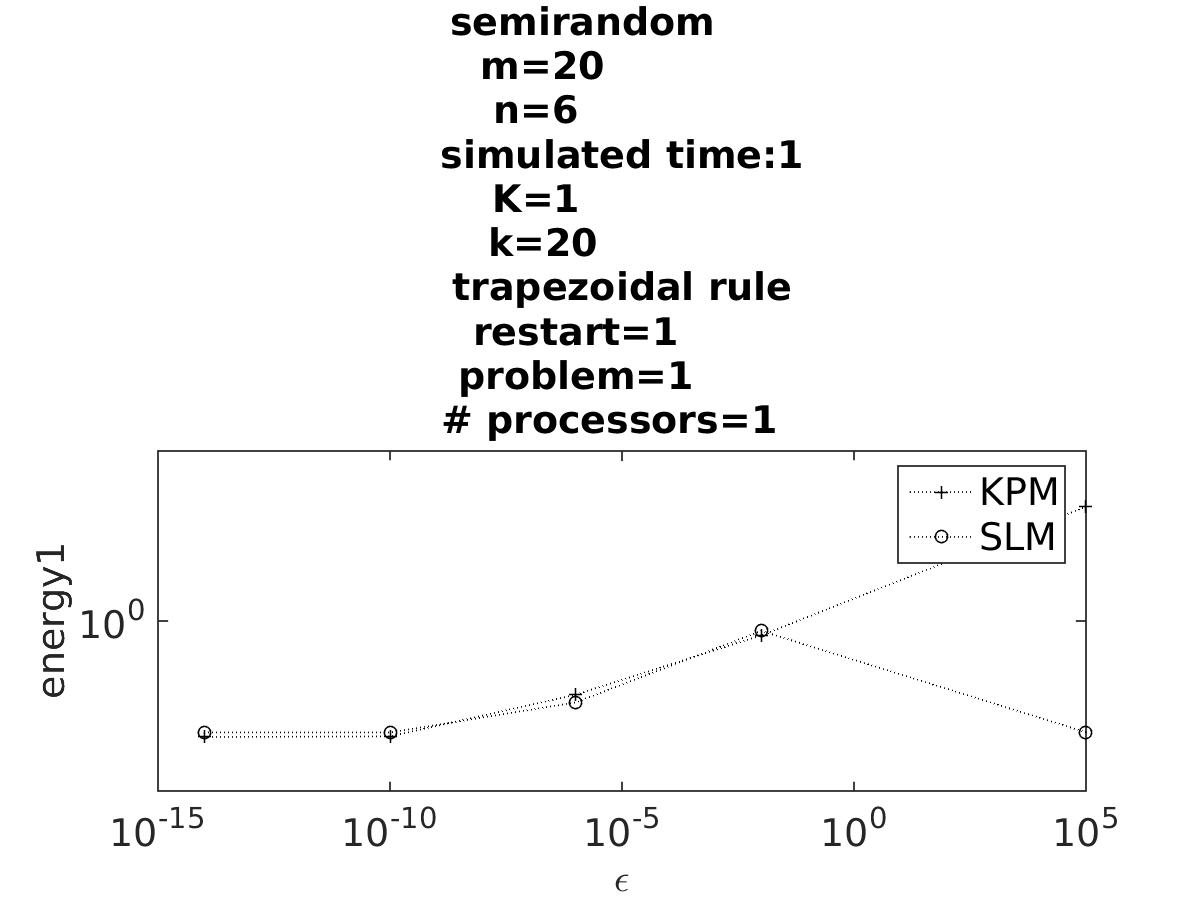
\includegraphics[width=\textwidth]{../MATLAB/fig/compareEnergy.jpg}
                \caption{ The difference in energy with and without restart. }
                \label{fig:compareEnergy}
        \end{subfigure}
        ~
        \begin{subfigure}[b]{0.45\textwidth}
                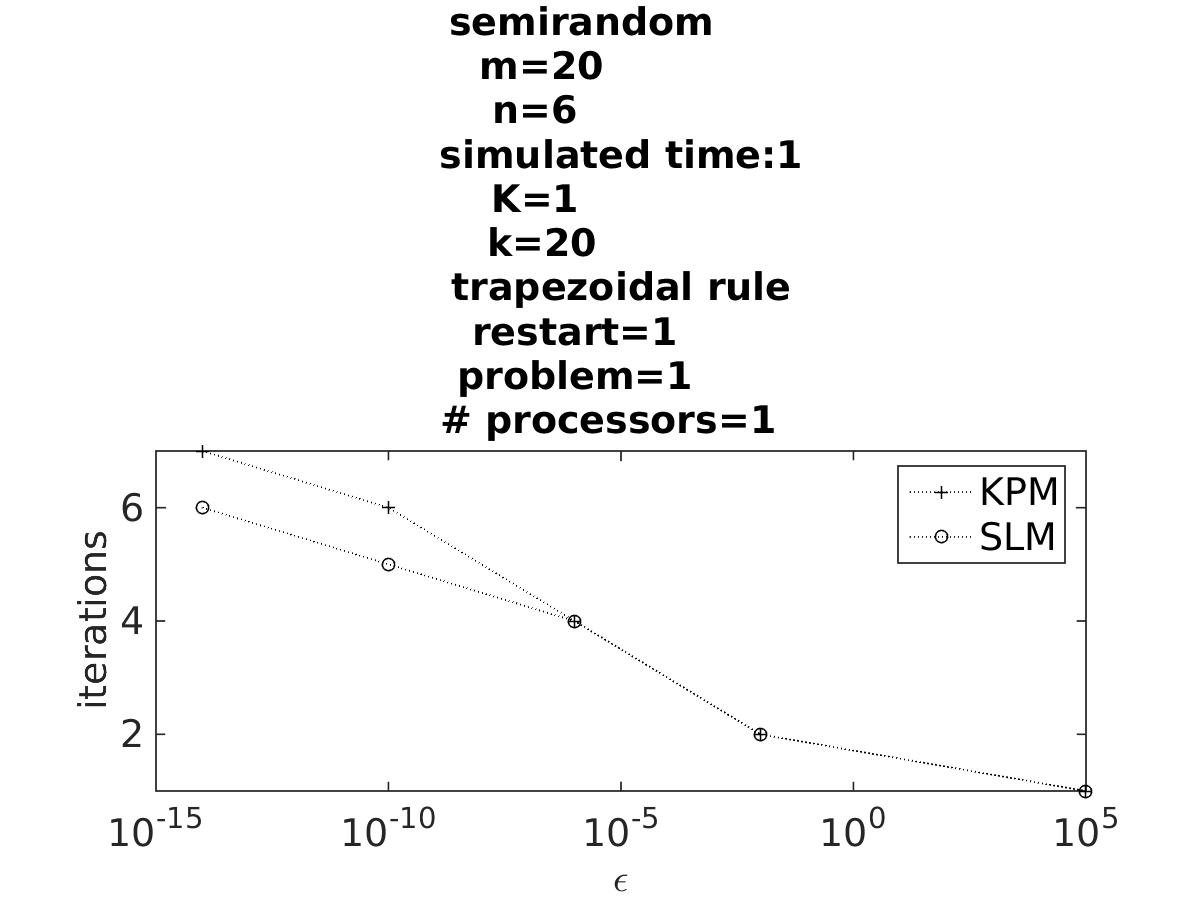
\includegraphics[width=\textwidth]{../MATLAB/fig/compareIter.jpg}
                \caption{ The number of iterations performed with and without restarting.  }
                \label{fig:compareIter}
        \end{subfigure}
        \caption{ The figure shows how the different methods change the energy with and without restarting.  }
        \label{fig:compare}
\end{figure}

The figures above implies that restarting the symplectic Lanczos method does indeed not change the energy. But for Arnoldi's method it changes quite a bit. 

\begin{figure}[H]
        \centering
        \begin{subfigure}[b]{0.45\textwidth}
                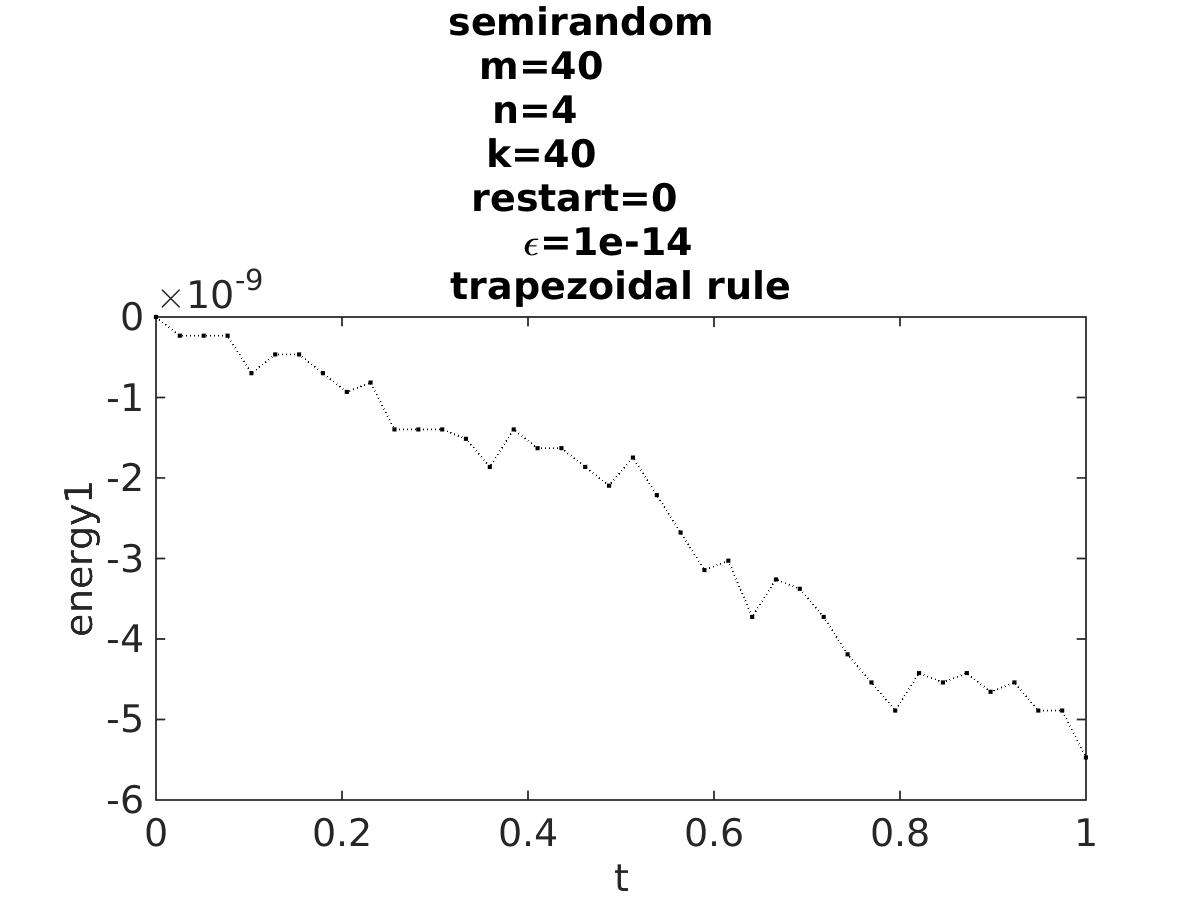
\includegraphics[width=\textwidth]{../MATLAB/fig/energytestrestart0.jpg}
                \caption{ Without restart. }
                \label{fig:energytestrestart0}
        \end{subfigure}
        ~
        \begin{subfigure}[b]{0.45\textwidth}
                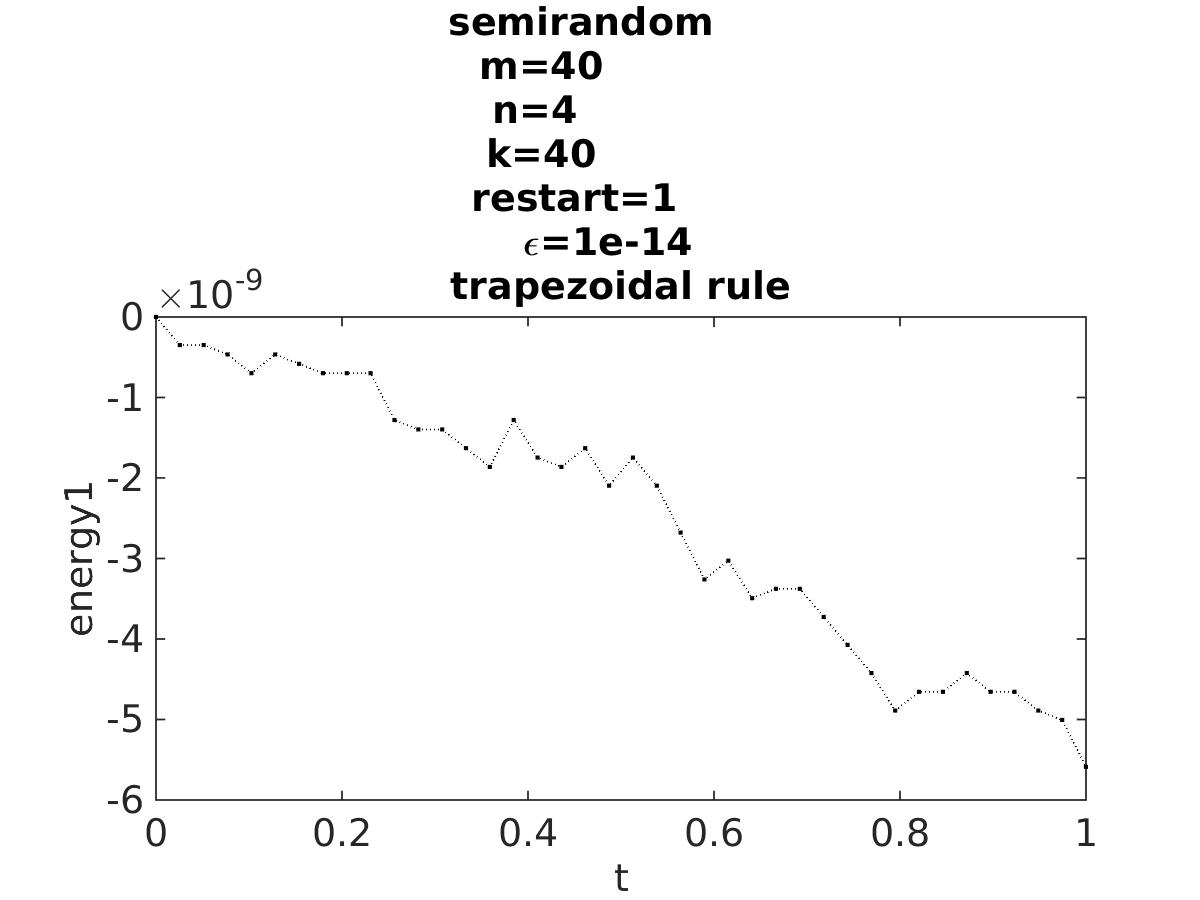
\includegraphics[width=\textwidth]{../MATLAB/fig/energytestrestart1.jpg}
                \caption{ With restart, the number of iterations $= 47$ }
                \label{fig:energytestrestart1}
        \end{subfigure}
        \caption{ The figures shows the change in energy over time.}
        \label{fig:energytestrestart}
\end{figure}
The figure above shows very little change in energy with SLM, with and without several restarts. \\

The figures below shows the same as figure \ref{fig:energytestrestart}, but with KPM instead of SLM. 

\begin{figure}[H]
        \centering
        \begin{subfigure}[b]{0.45\textwidth}
                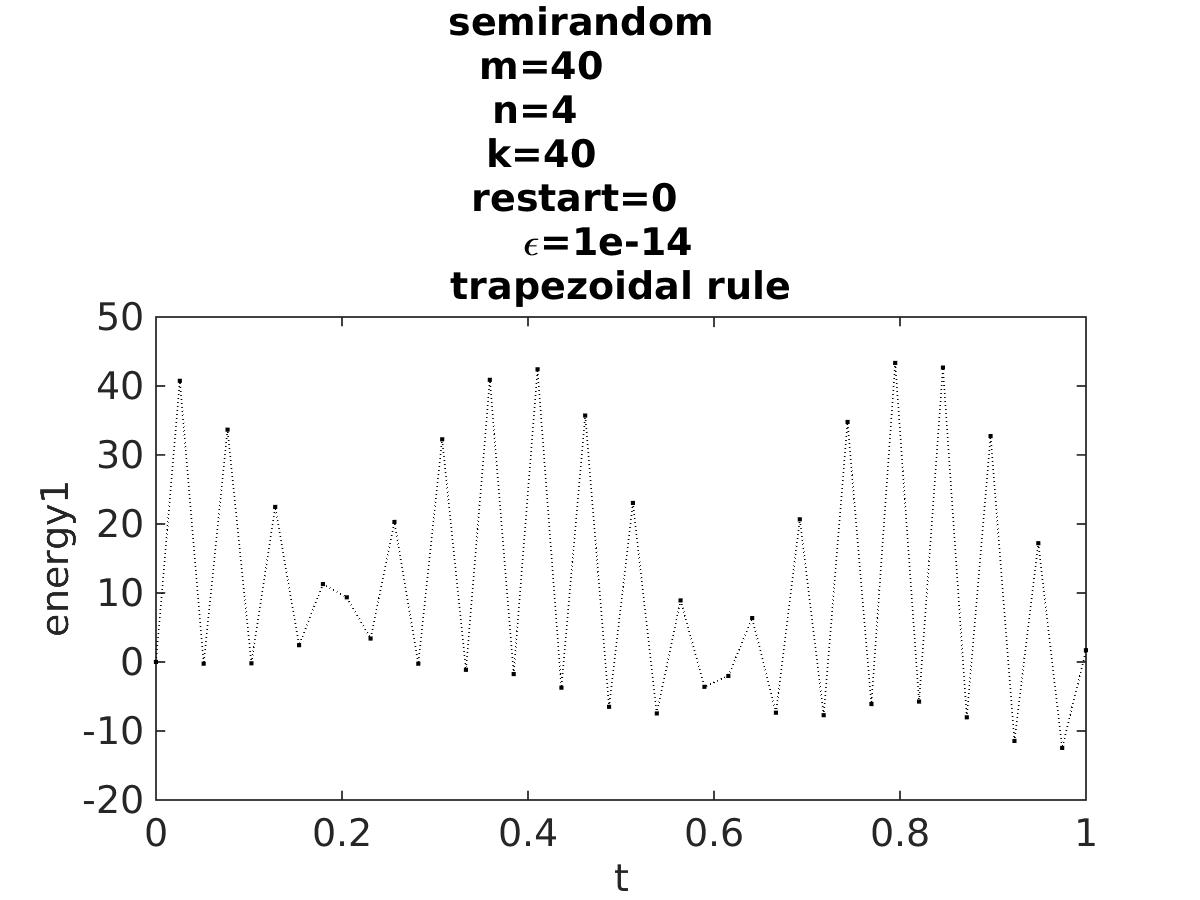
\includegraphics[width=\textwidth]{../MATLAB/fig/energyarnrestart0.jpg}
                \caption{  Without restart. }
                \label{fig:energyarnrestart0}
        \end{subfigure}%
        ~
        \begin{subfigure}[b]{0.45\textwidth}
                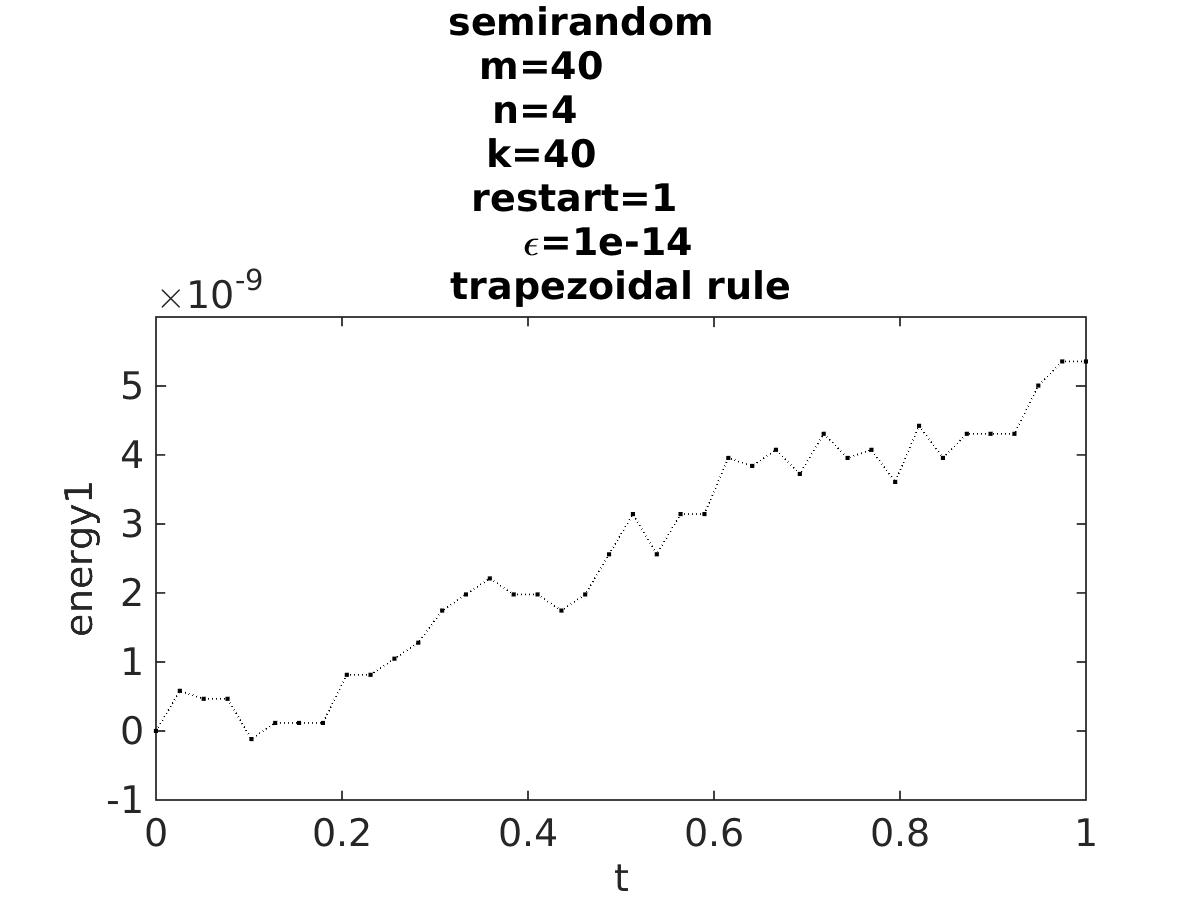
\includegraphics[width=\textwidth]{../MATLAB/fig/energyarnrestart1.jpg}
                \caption{ With restart, the number of iterations $ = 48$ }
                \label{fig:energyarnrestart1}
        \end{subfigure}
        \caption{ Figures showing the change in energy over time. }
        \label{fig:energyarnrestart}
\end{figure}

When comparing figure \ref{fig:energytestrestart0} and \ref{fig:energytestrestart1} it becomes clear that SLM's does not alter the energy significantly when performing the restart. Figure \ref{fig:energyarnrestart0} and \ref{fig:energyarnrestart1} shows that this is not the case for KPM.\\

%!!!!!!!!!!!!!!!!Burde jeg gjøre det samme for feilen?(JA)!!!!!!!!!!!!!!!!!!!!!!!!!!!!!!!\\

%!!!!!!!!!!!!!!!!!!!!!!!ER dette overbevisende nok?!!!!!!!!!!!!!!!!!!!!!!!!!!!!!\\
%%%%%%%%%%%%%%%%%%%%%%%%%%%%%%%%%%%%%%%%%%%%%%%%%%%%%%%%%%%%%%%%%%%%%%%%%%%%%%%%%%%%%%%%%%%%%%%%%%%%%%%%%%%%%%%%
\chapter{Some interesting results}
%%%%%%%%%%%%%%%%%%%%%%%%%%%%%%%%%%%%%%%%%%%%%%%%%%%%%%%%%%%%%%%%%%%%%%%%%%%%%%%%%%%%%%%%%%%%%%%%%%%%%%%%%%%%%%%
The energy has already been considered quite thoroughly, but there are still interesting factors to consider. This chapter will discus how the different methods compare in relation to computation time, number of iterations, and error. This will be done with  \texttt{wave} and \texttt{semirandom} both with constant and varying energy


\section{constant energy with the wave equation}
%%%%%%%%%%%%%%%%%%%%%%%%%%%%%%%%%%%%%%%%%%%%%%%%%%%%%%%%%%%%%%%%%%%%%%%%%%%%%%%%%%%%%%%%%%%%%%%%%%%%%%%%%%%%%%%
 The \texttt{wave} framework will be used due to the need for comparing the difficulty of solving the problem with different sizes.\\
%!!!!!!!!!!!!!!!!!!!!!Dette må gjøres for andre problemer, dette er jo bare teit!!!!!!!!!!!!!!!!!!!!!!!\\



\begin{figure}[H]
        \centering
        \begin{subfigure}[b]{0.45\textwidth}
                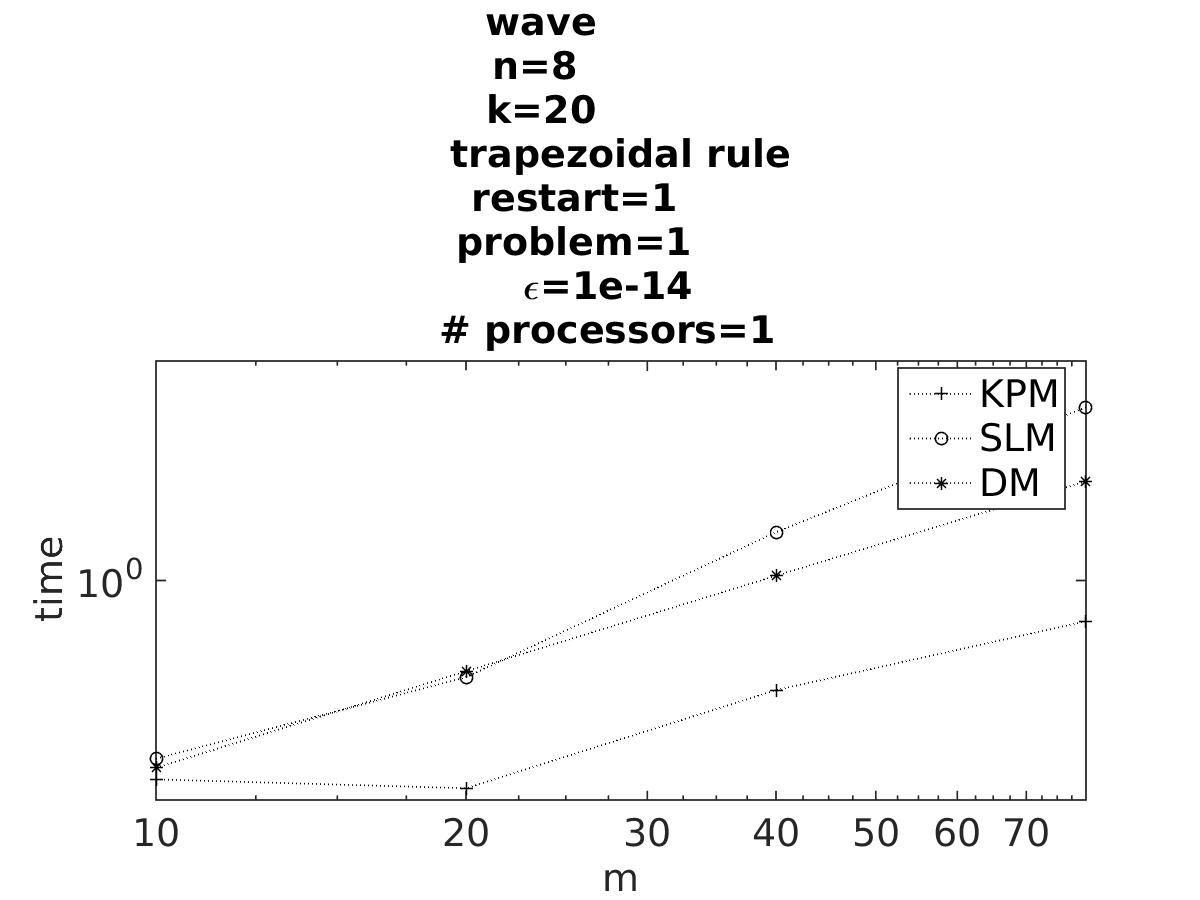
\includegraphics[width=\textwidth]{../MATLAB/fig/resulttimem.jpg}
                \caption{  }
                \label{fig:resulttimem}
        \end{subfigure}
        ~
        \begin{subfigure}[b]{0.45\textwidth}
                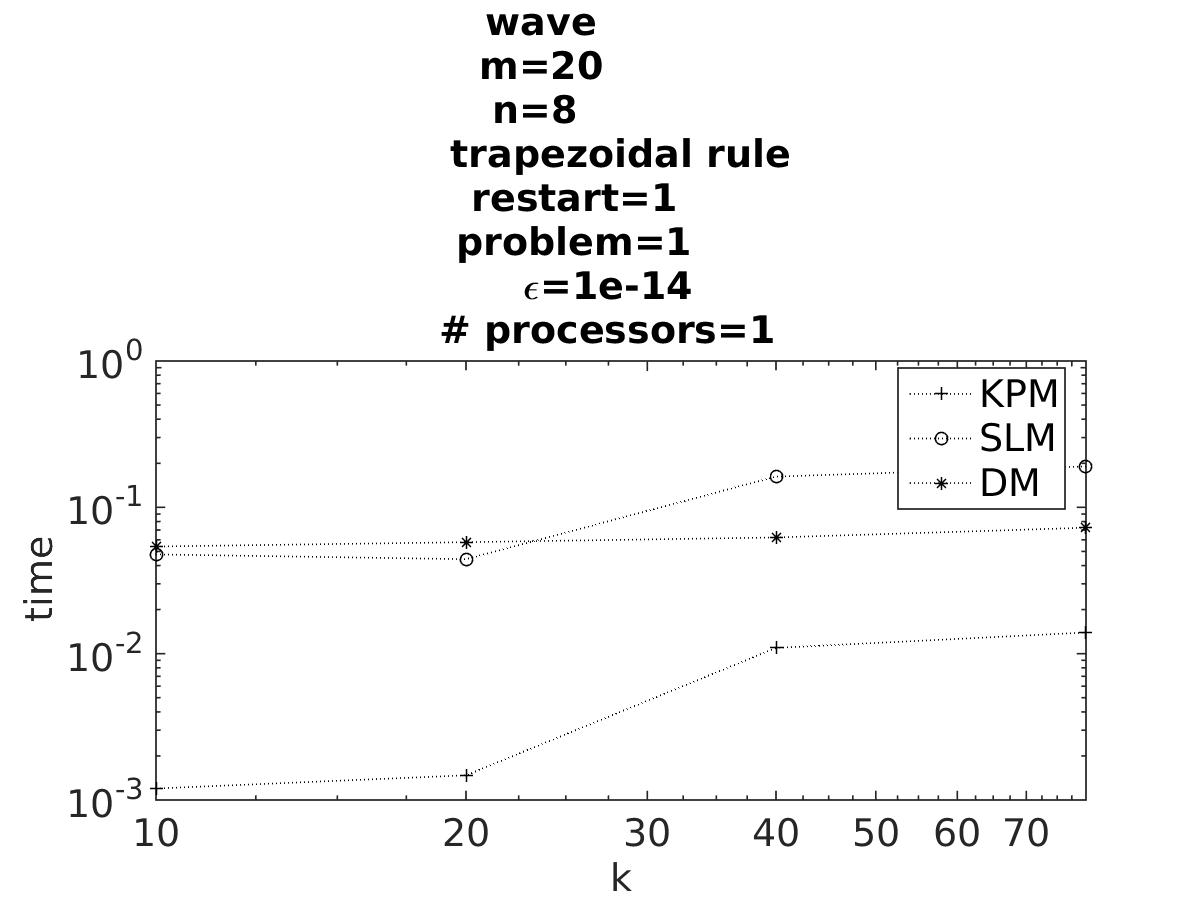
\includegraphics[width=\textwidth]{../MATLAB/fig/resulttimek.jpg}
                \caption{  }
                \label{fig:resulttimek}
        \end{subfigure}
        \caption{ For both cases KPM is faster than the other, and with DM faster than SLM.  }
        \label{fig:resulttime}
\end{figure}



\begin{figure}[H]
        \centering

                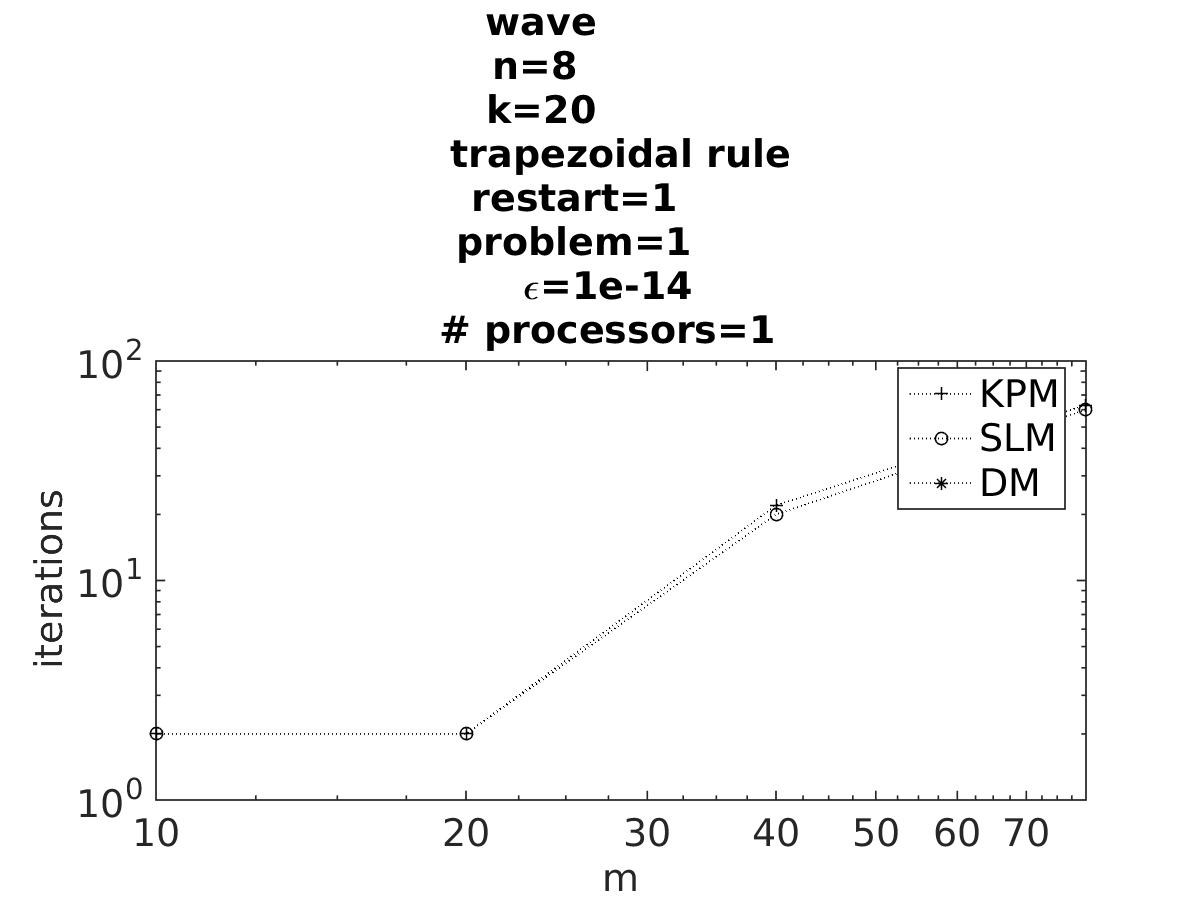
\includegraphics[width=0.45\textwidth]{../MATLAB/fig/resultiter.jpg}
        \label{fig:resultiter}
        \caption{The number of iterations are almost equal for the two methods.}
\end{figure}

\begin{figure}[H]
        \centering
        \begin{subfigure}[b]{0.45\textwidth}
                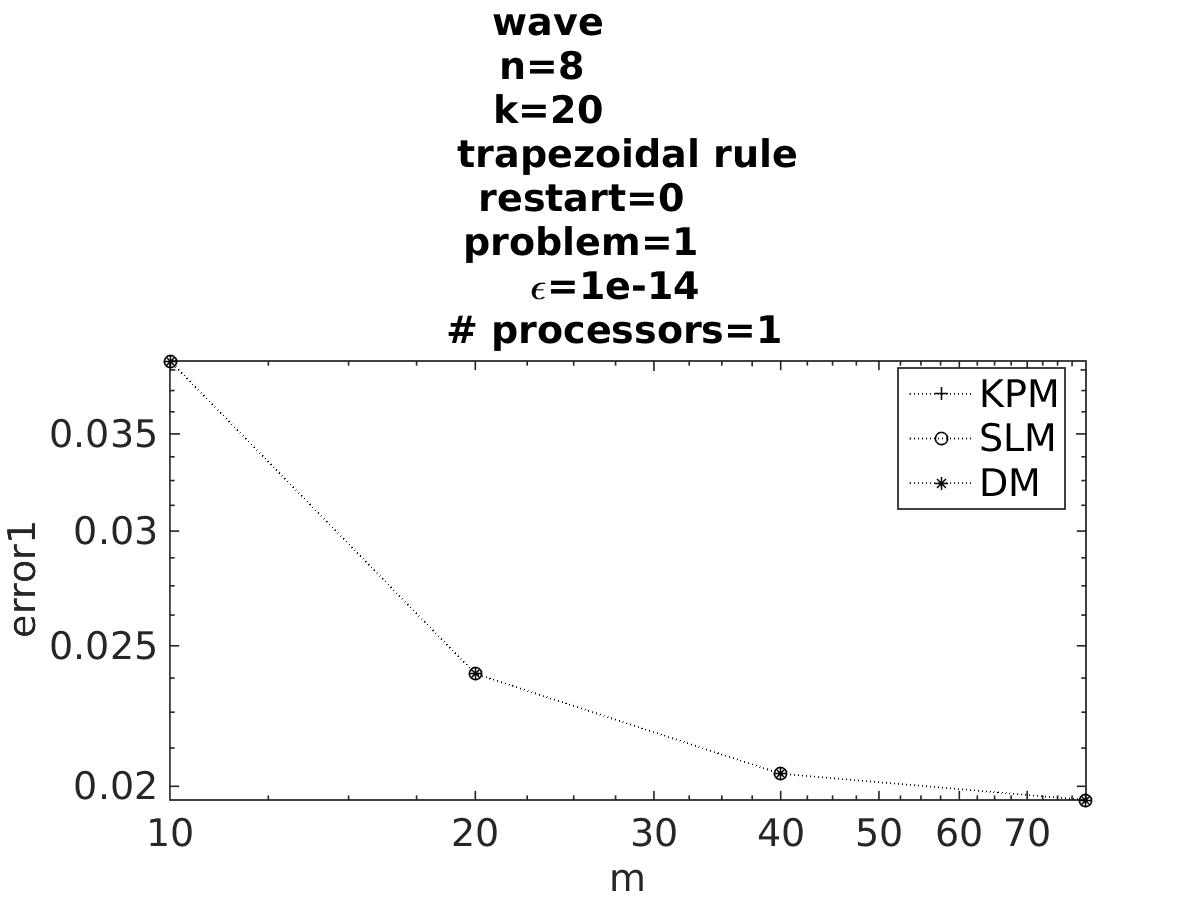
\includegraphics[width=\textwidth]{../MATLAB/fig/resulterrorr.jpg}
                \caption{  }
                \label{fig:resulterror1}
        \end{subfigure}
        ~
        \begin{subfigure}[b]{0.45\textwidth}
                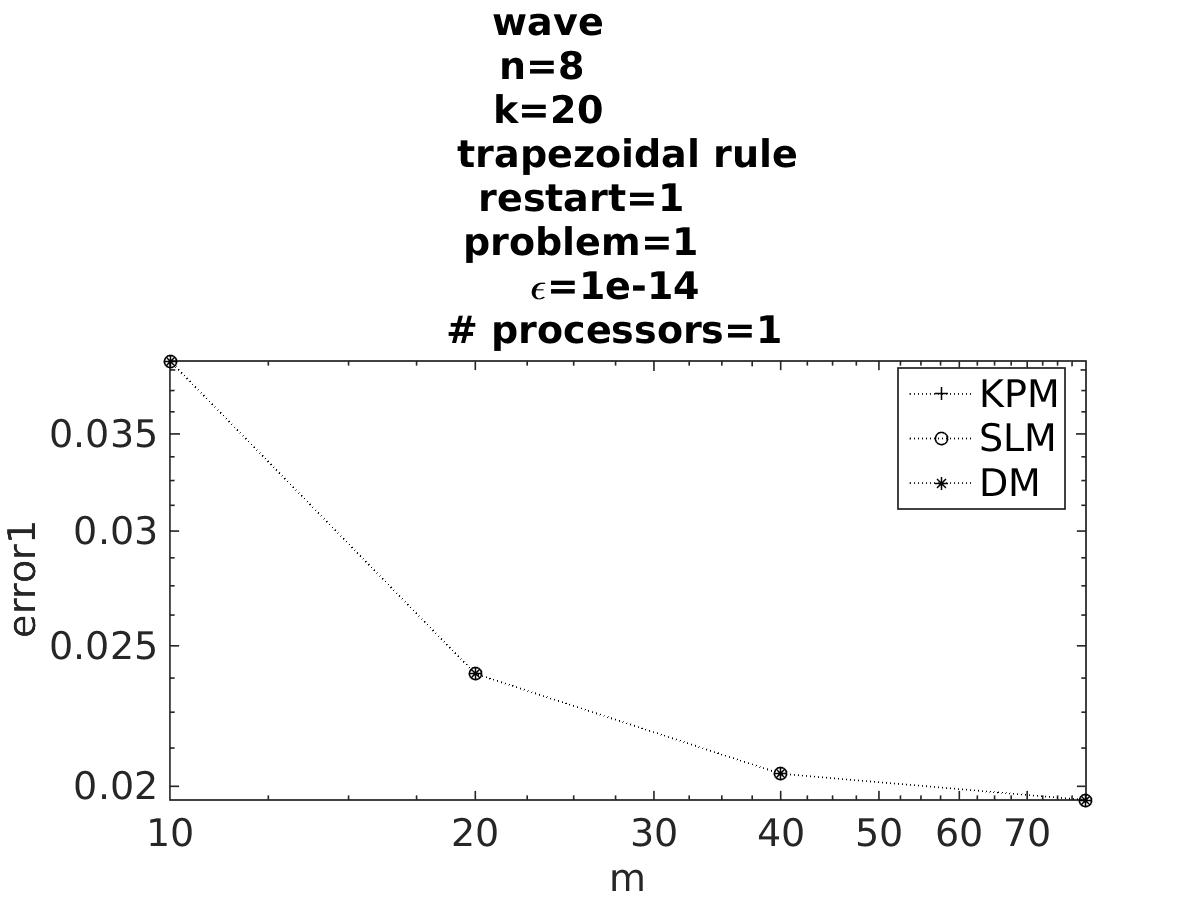
\includegraphics[width=\textwidth]{../MATLAB/fig/resulterror.jpg}
                \caption{  }
                \label{fig:resulterror2}
        \end{subfigure}
        \caption{ The error is nearly identical.  }
        \label{fig:resulterror}
\end{figure}


\begin{figure}[H]
        \centering
        \begin{subfigure}[b]{0.45\textwidth}
                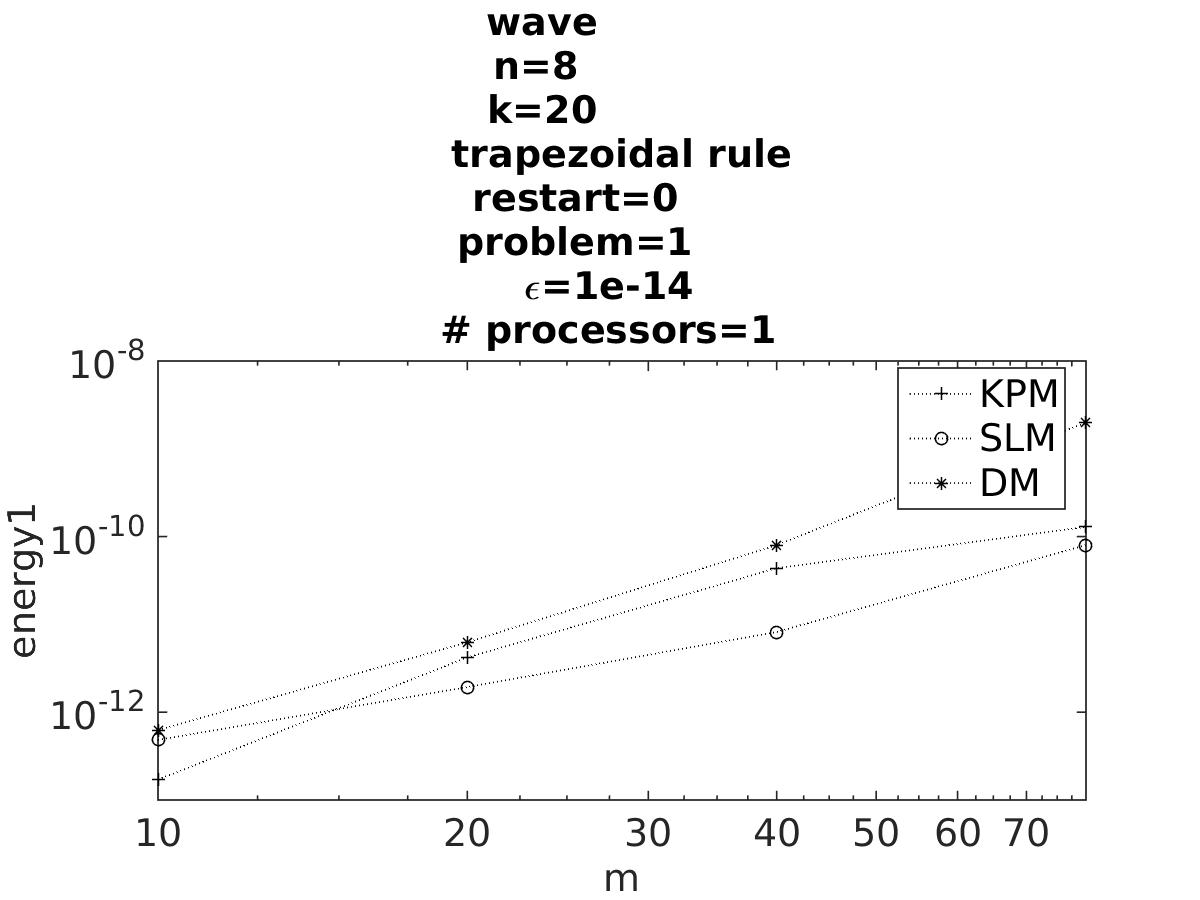
\includegraphics[width=\textwidth]{../MATLAB/fig/resultenergyr.jpg}
                \caption{  }
                \label{fig:resultenergy1}
        \end{subfigure}
        ~
        \begin{subfigure}[b]{0.45\textwidth}
                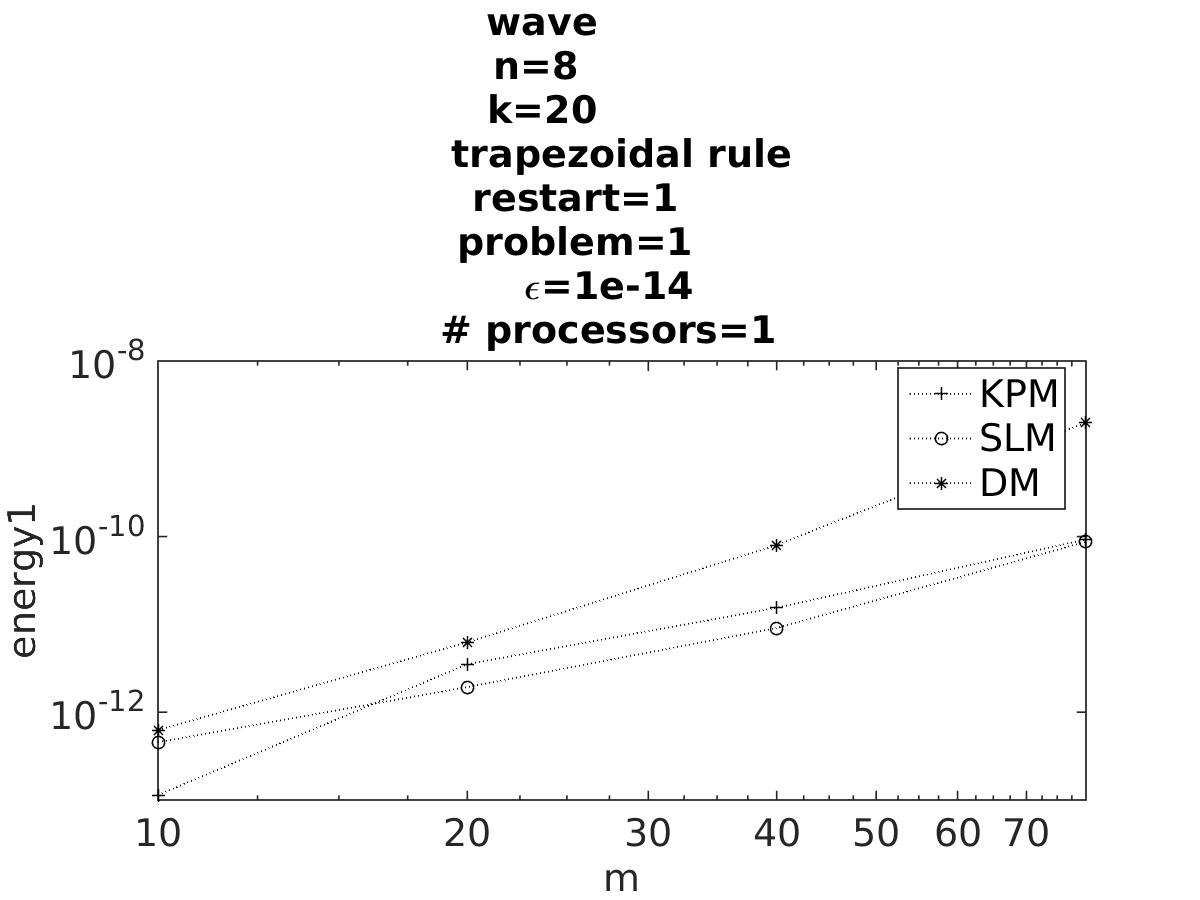
\includegraphics[width=\textwidth]{../MATLAB/fig/resultenergy.jpg}
                \caption{  }
                \label{fig:resultenergy2}
        \end{subfigure}
        \caption{ SLM and KPM has the best energy estimation, with DM not far behind. }
        \label{fig:resultenergy}
\end{figure}

It is pretty clear that the figure in this section gives no useful information about the difference between the two methods in other tings than computation time.



\section{constant energy with the semirandom equation}
%%%%%%%%%%%%%%%%%%%%%%%%%%%%%%%%%%%%%%%%%%%%%%%%%%%%%%%%%%%%%%%%%%%%%%%%%%%%%%%%%%%%%%%%%%%%%%%%%%%%%%%



\begin{figure}[H]
        \centering
        \begin{subfigure}[b]{0.45\textwidth}
                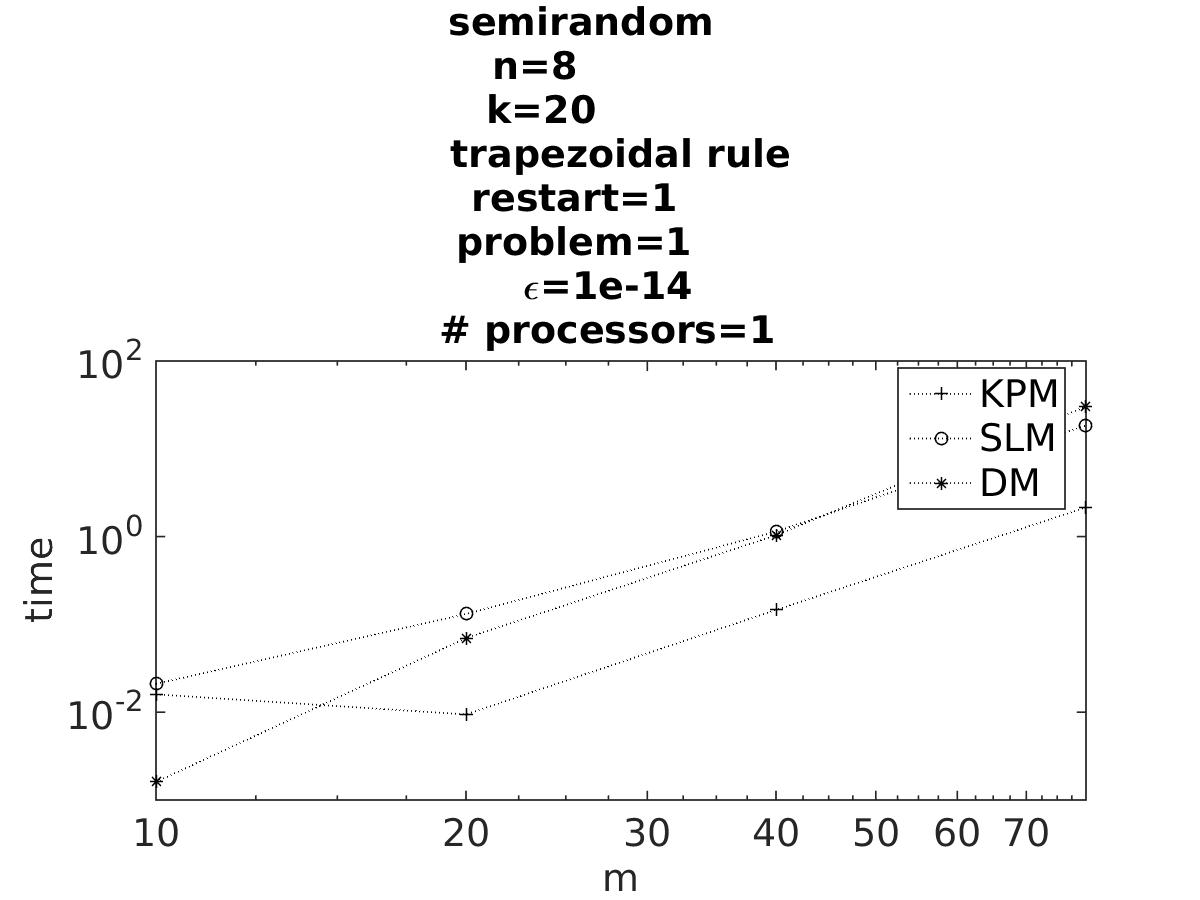
\includegraphics[width=\textwidth]{../MATLAB/fig/sresulttimem.jpg}
                \caption{  }
                \label{fig:sresulttimem}
        \end{subfigure}
        ~
        \begin{subfigure}[b]{0.45\textwidth}
                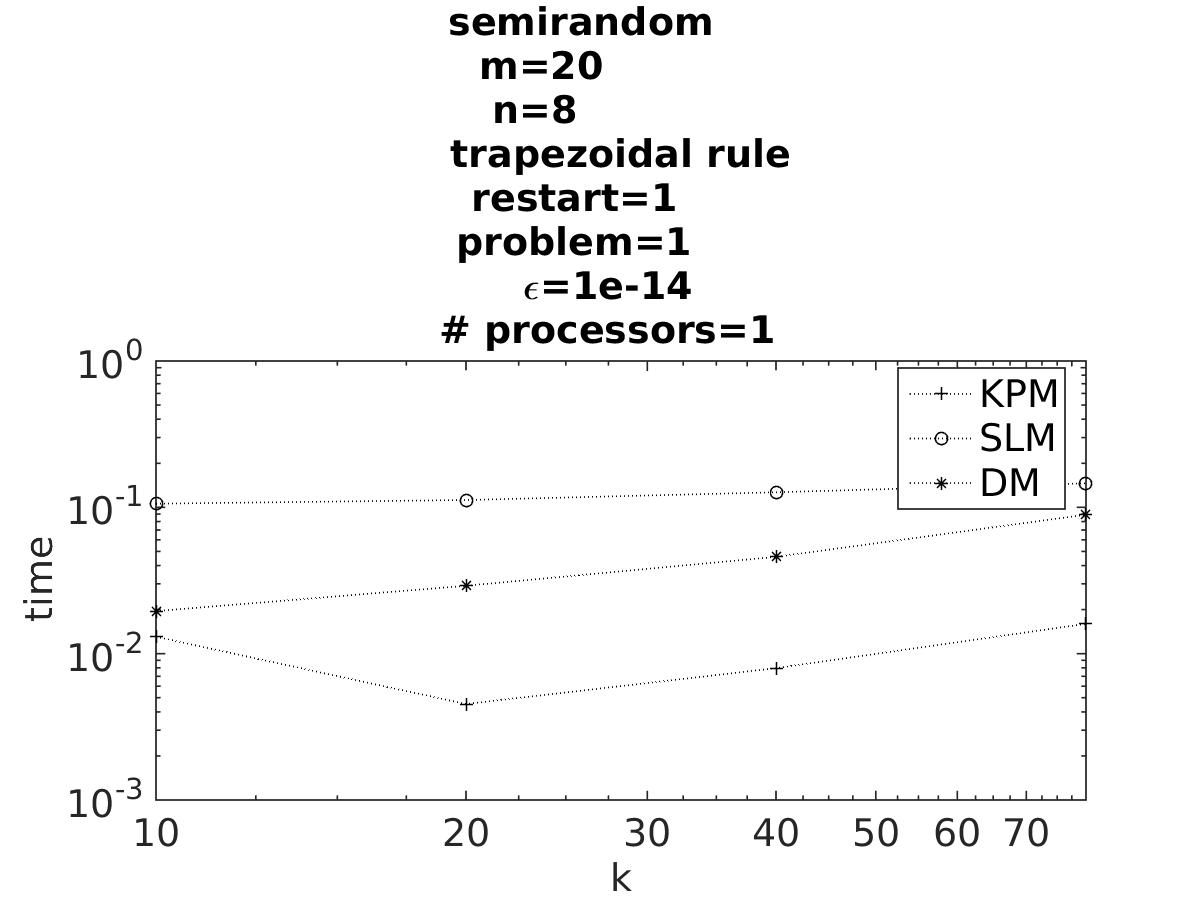
\includegraphics[width=\textwidth]{../MATLAB/fig/sresulttimek.jpg}
                \caption{  }
                \label{fig:sresulttimek}
        \end{subfigure}
        \caption{ For both cases KPM is faster than the other, and with DM faster than SLM.  }
        \label{fig:sresulttime}
\end{figure}



\begin{figure}[H]
        \centering

                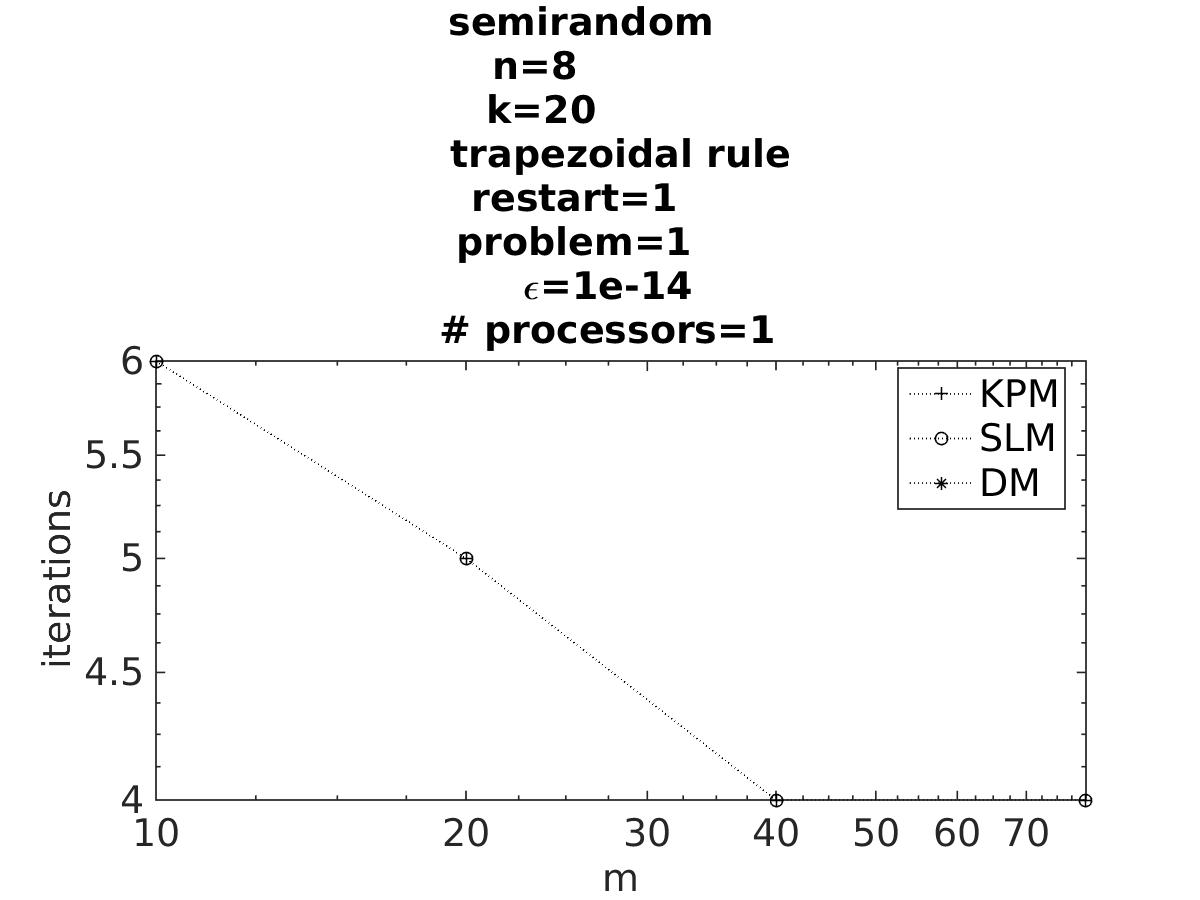
\includegraphics[width=0.45\textwidth]{../MATLAB/fig/sresultiter.jpg}
        \label{fig:sresultiter}
        \caption{The number of iterations are almost equal for the two methods.}
\end{figure}

\begin{figure}[H]
        \centering
        \begin{subfigure}[b]{0.45\textwidth}
                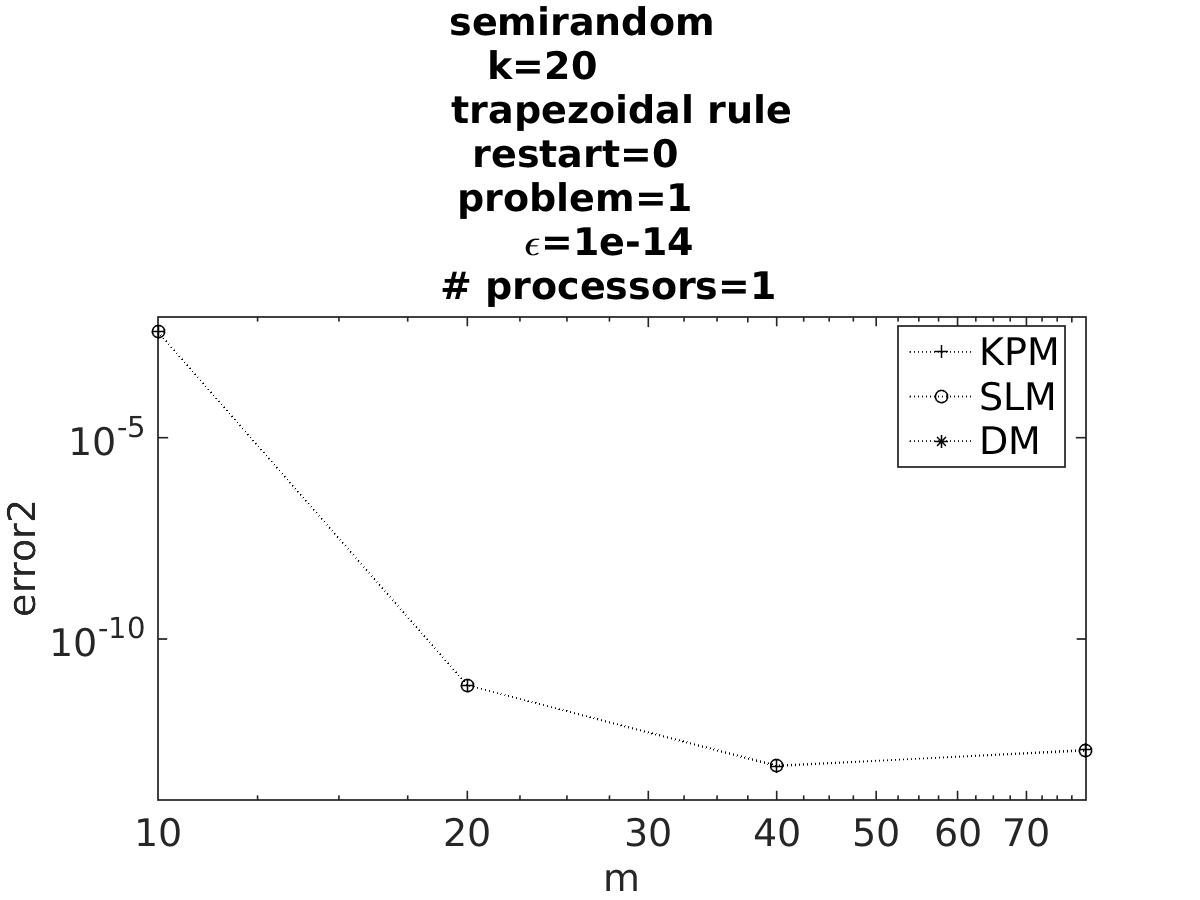
\includegraphics[width=\textwidth]{../MATLAB/fig/sresulterrorr.jpg}
                \caption{  }
                \label{fig:sresulterror1}
        \end{subfigure}
        ~
        \begin{subfigure}[b]{0.45\textwidth}
                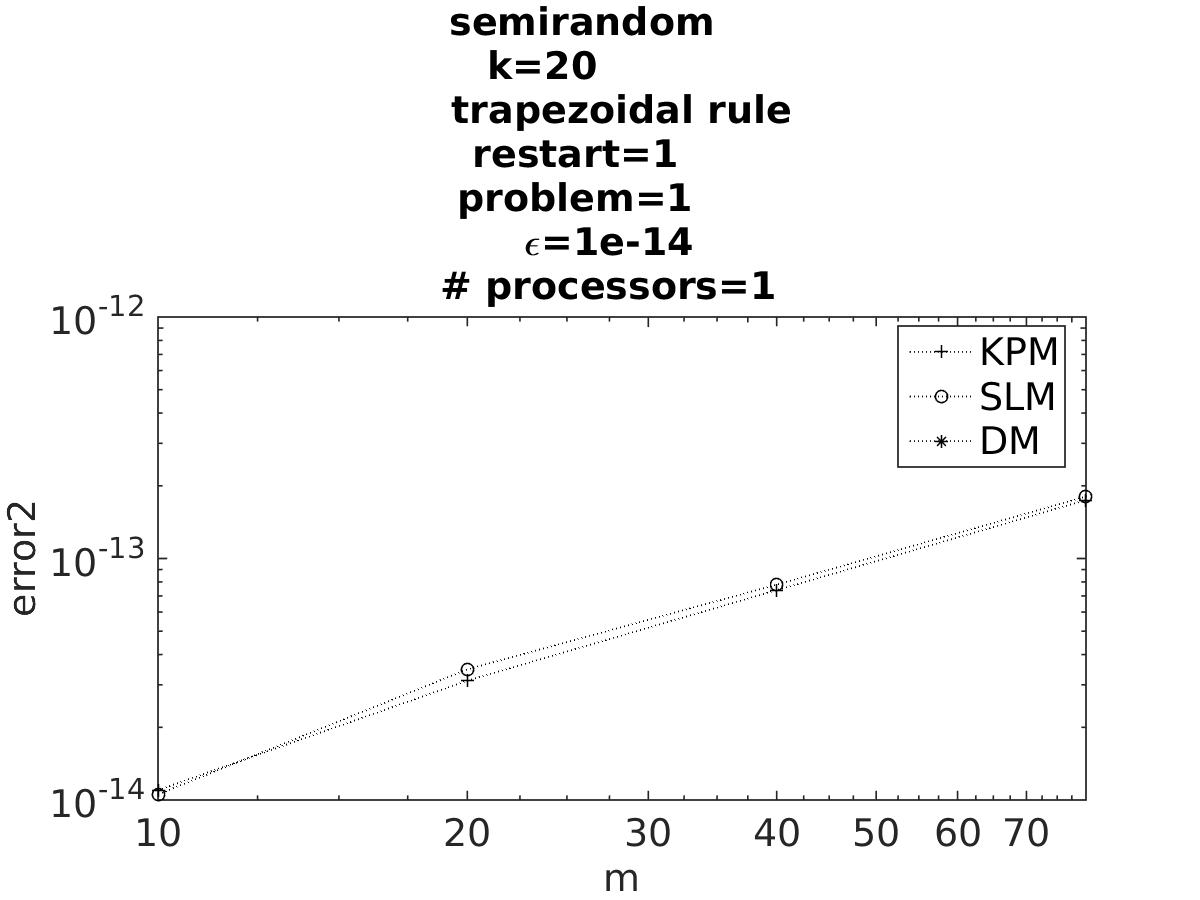
\includegraphics[width=\textwidth]{../MATLAB/fig/sresulterror.jpg}
                \caption{  }
                \label{fig:sresulterror2}
        \end{subfigure}
        \caption{ The error is nearly identical.  }
        \label{fig:sresulterror}
\end{figure}


\begin{figure}[H]
        \centering
        \begin{subfigure}[b]{0.45\textwidth}
                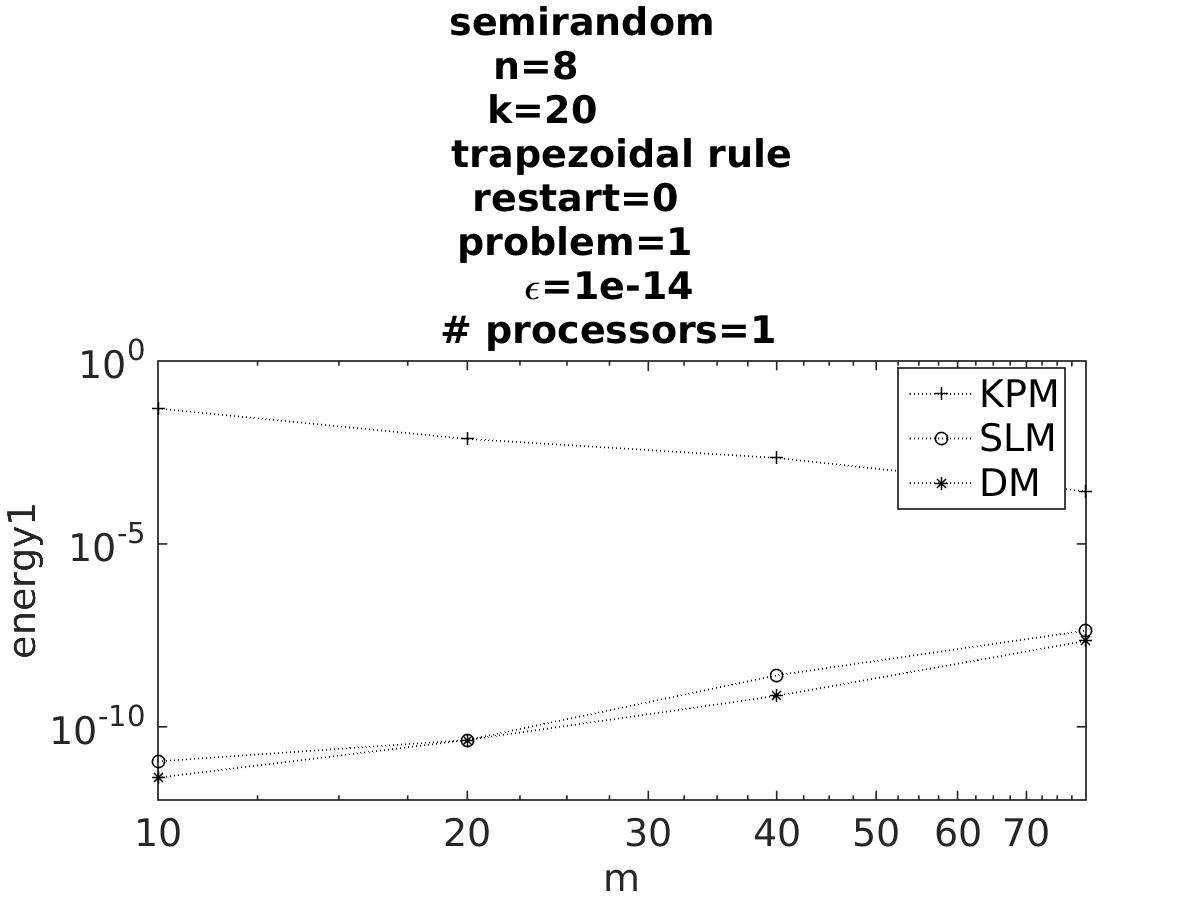
\includegraphics[width=\textwidth]{../MATLAB/fig/sresultenergyr.jpg}
                \caption{  }
                \label{fig:sresultenergy1}
        \end{subfigure}
        ~
        \begin{subfigure}[b]{0.45\textwidth}
                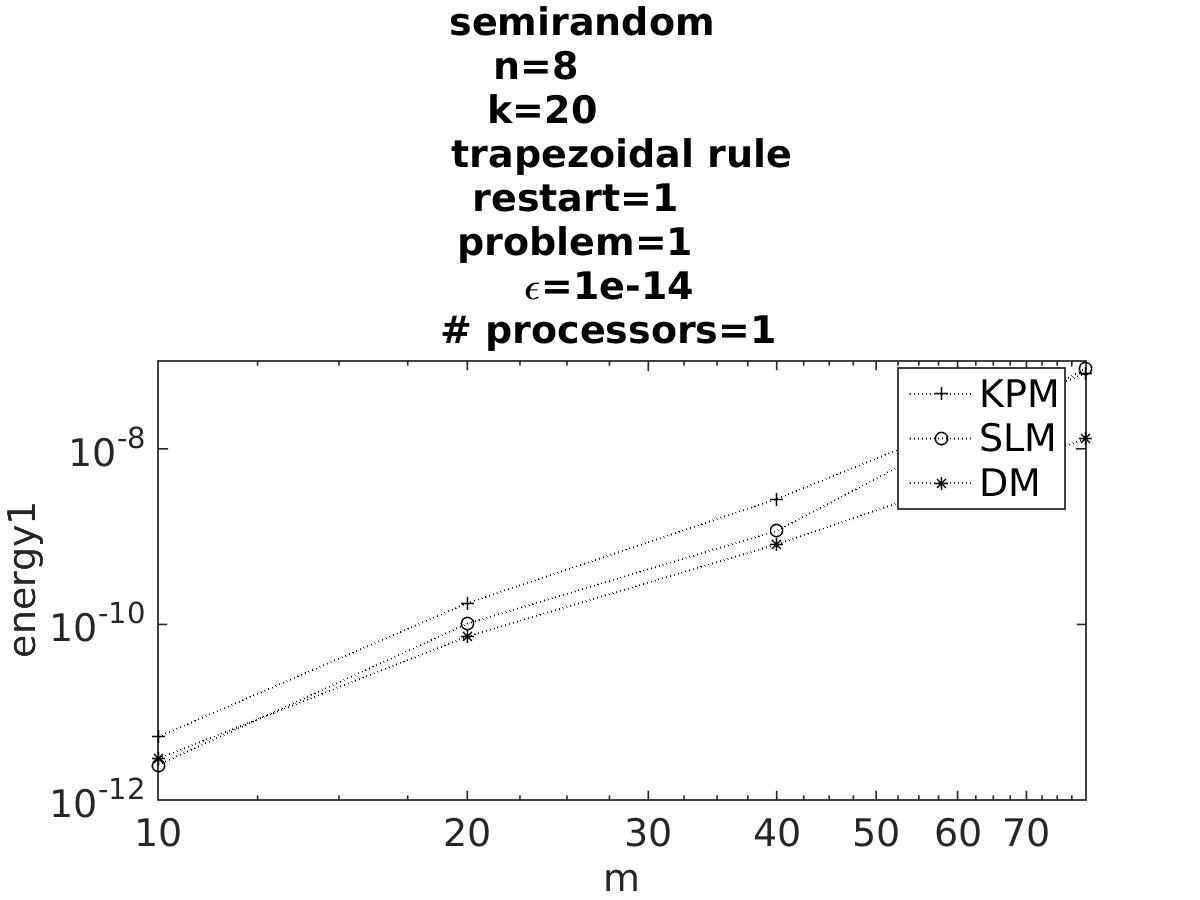
\includegraphics[width=\textwidth]{../MATLAB/fig/sresultenergy.jpg}
                \caption{  }
                \label{fig:sresultenergy2}
        \end{subfigure}
        \caption{ SLM and KPM has the best energy estimation, with DM not far behind. }
        \label{fig:sresultenergy}
\end{figure}

The figures in this section shows a little better how the energy for the different methods change, but the error is apparently useless in this setting due to it being the difference between two calculated numbers, and not the analytical solution. 

\section{Varying energy with the wave equation}
%%%%%%%%%%%%%%%%%%%%%%%%%%%%%%%%%%%%%%%%%%%%%%%%%%%%%%%%%%%%%%%%%%%%%%%%%%%%%%%%%%%%%%%%%%%%%%%%%%%%%%%
\begin{figure}[H]
        \centering
        \begin{subfigure}[b]{0.45\textwidth}
                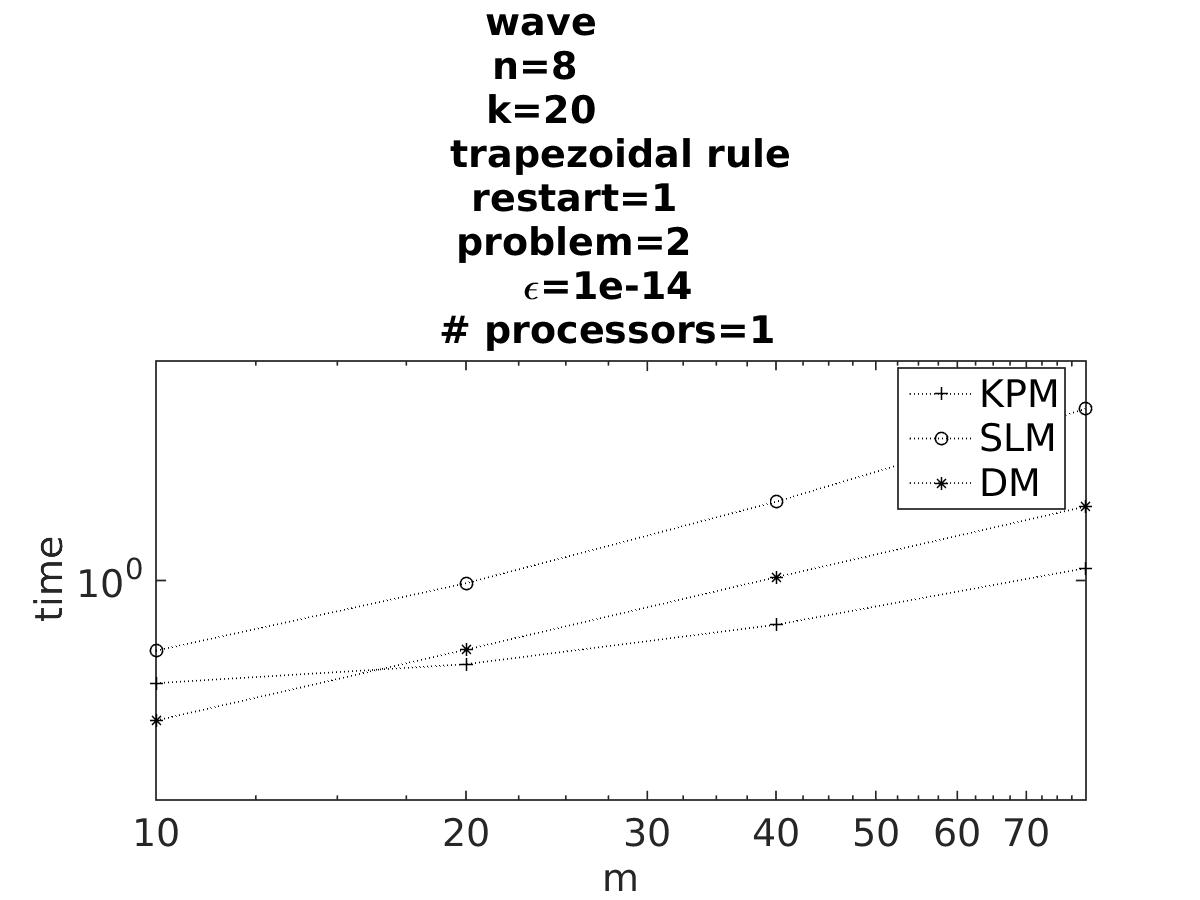
\includegraphics[width=\textwidth]{../MATLAB/fig/vresulttimem.jpg}
                \caption{  }
                \label{fig:vresulttimem}
        \end{subfigure}
        ~
        \begin{subfigure}[b]{0.45\textwidth}
                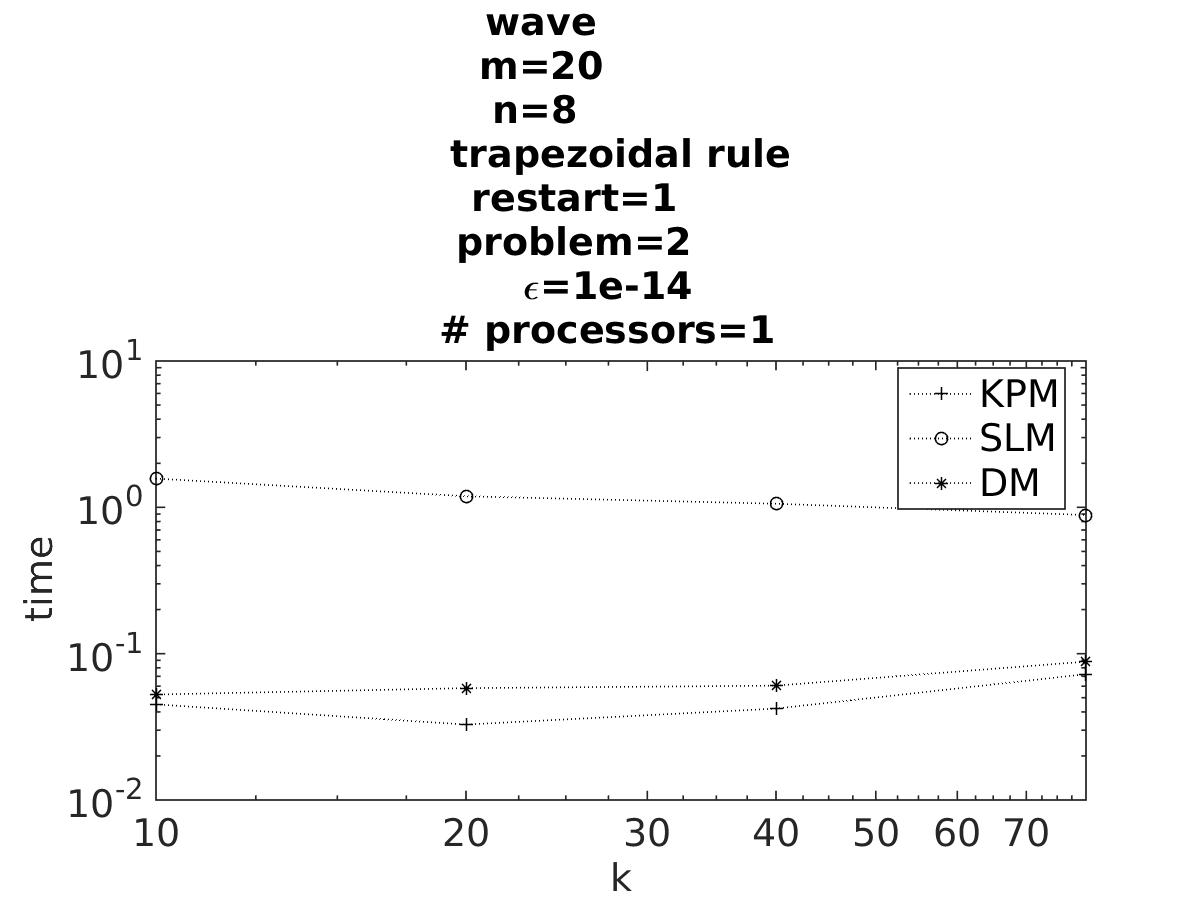
\includegraphics[width=\textwidth]{../MATLAB/fig/vresulttimek.jpg}
                \caption{  }
                \label{fig:vresulttimek}
        \end{subfigure}
        \caption{ For both cases KPM is faster than the other, and with DM faster than SLM.  }
        \label{fig:vresulttime}
\end{figure}



\begin{figure}[H]
        \centering

                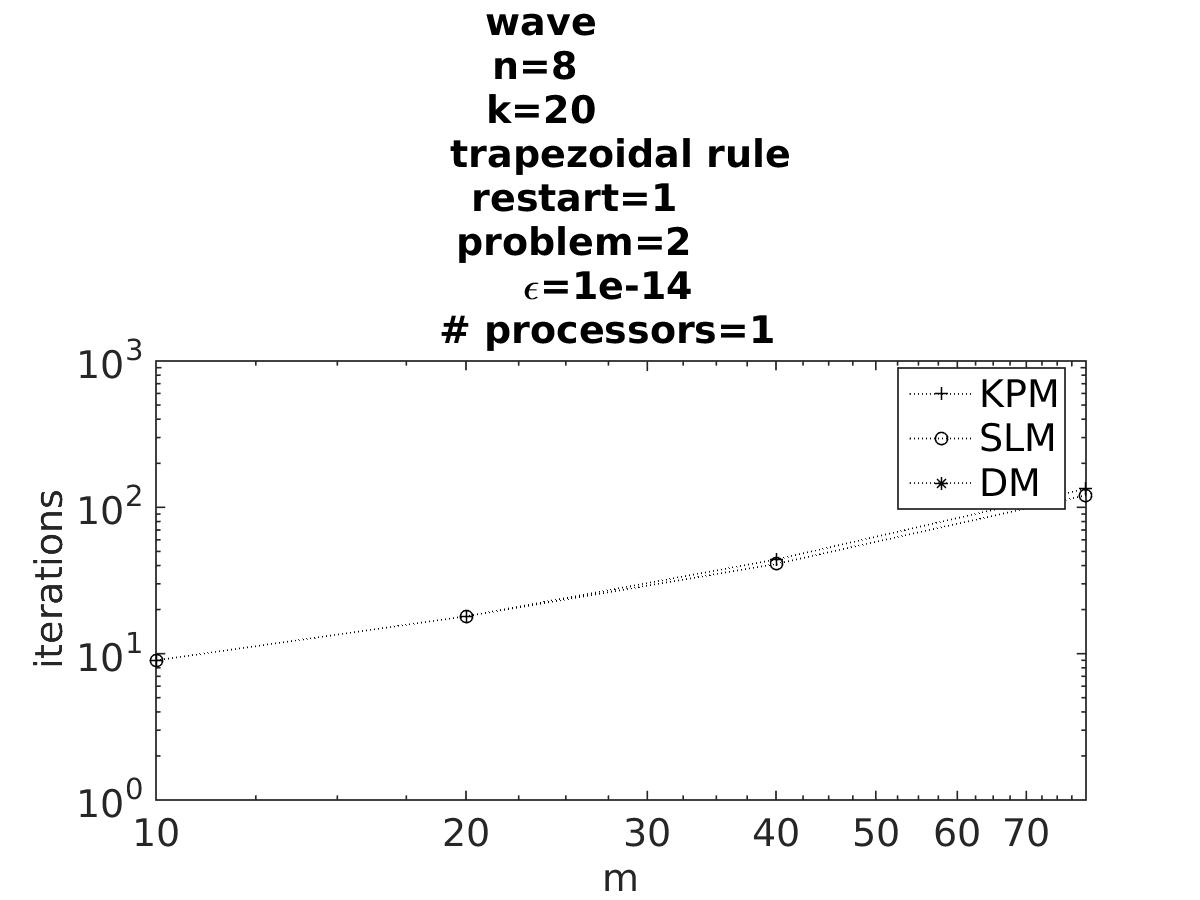
\includegraphics[width=0.45\textwidth]{../MATLAB/fig/vresultiter.jpg}
        \label{fig:vresultiter}
        \caption{The number of iterations are almost equal for the two methods.}
\end{figure}

\begin{figure}[H]
        \centering
        \begin{subfigure}[b]{0.45\textwidth}
                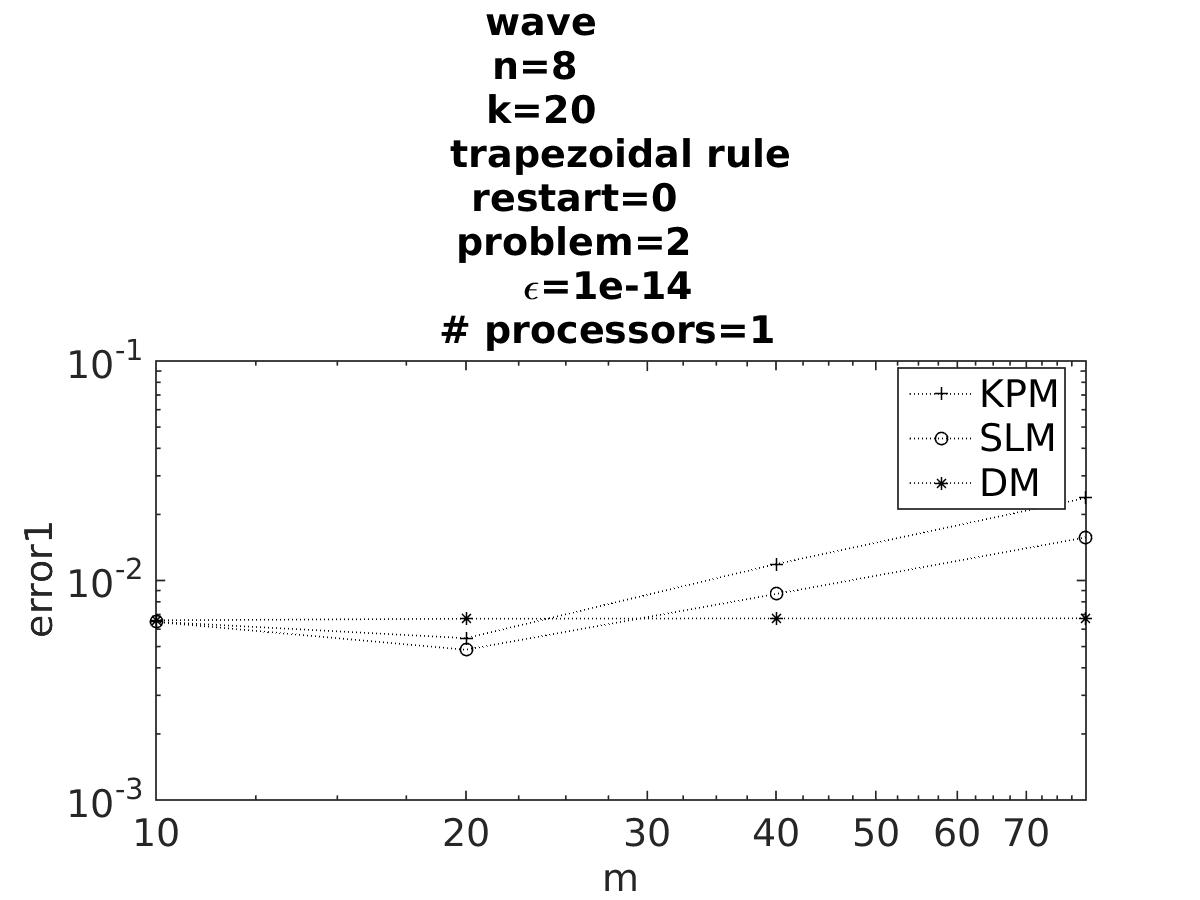
\includegraphics[width=\textwidth]{../MATLAB/fig/vresulterrorr.jpg}
                \caption{  }
                \label{fig:vresulterror1}
        \end{subfigure}
        ~
        \begin{subfigure}[b]{0.45\textwidth}
                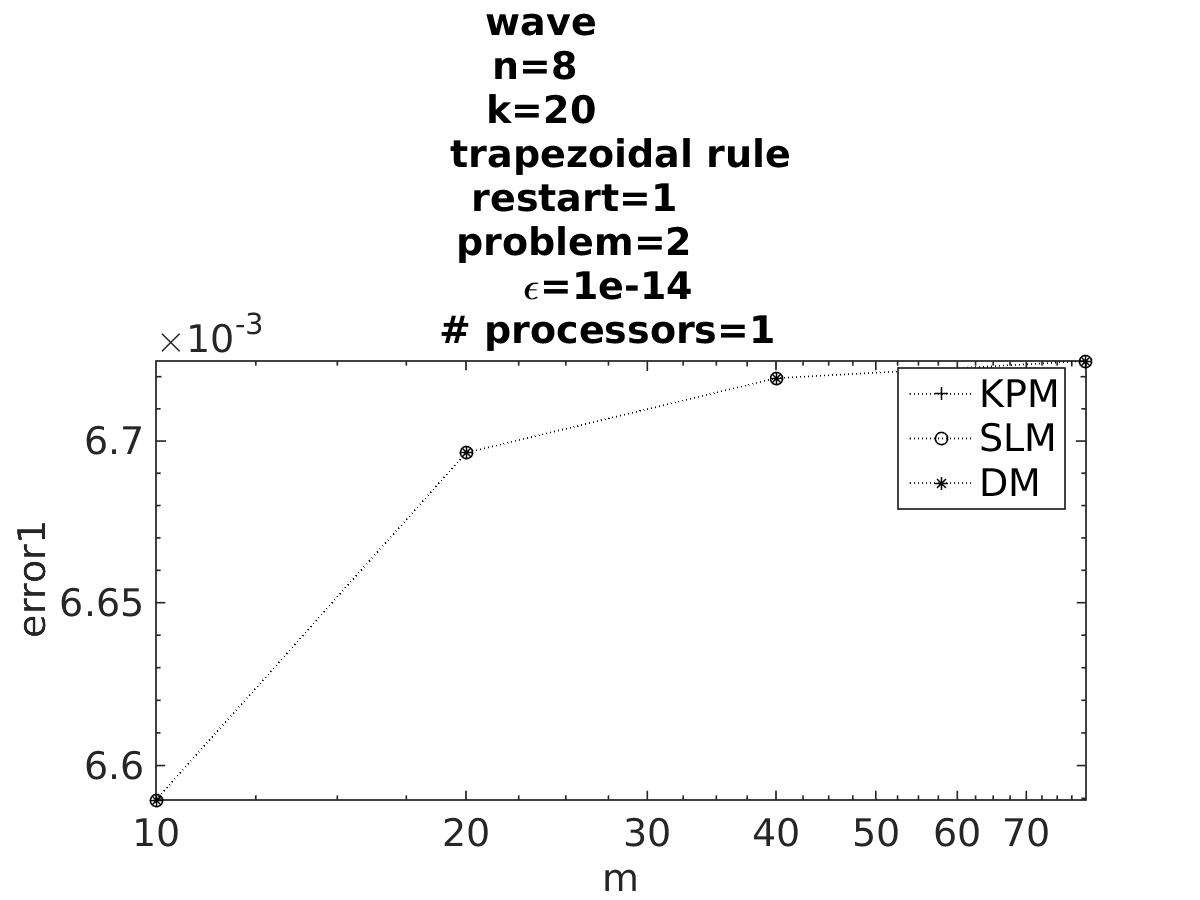
\includegraphics[width=\textwidth]{../MATLAB/fig/vresulterror.jpg}
                \caption{  }
                \label{fig:vresulterror2}
        \end{subfigure}
        \caption{ The error is nearly identical.  }
        \label{fig:vresulterror}
\end{figure}


\begin{figure}[H]
        \centering
        \begin{subfigure}[b]{0.45\textwidth}
                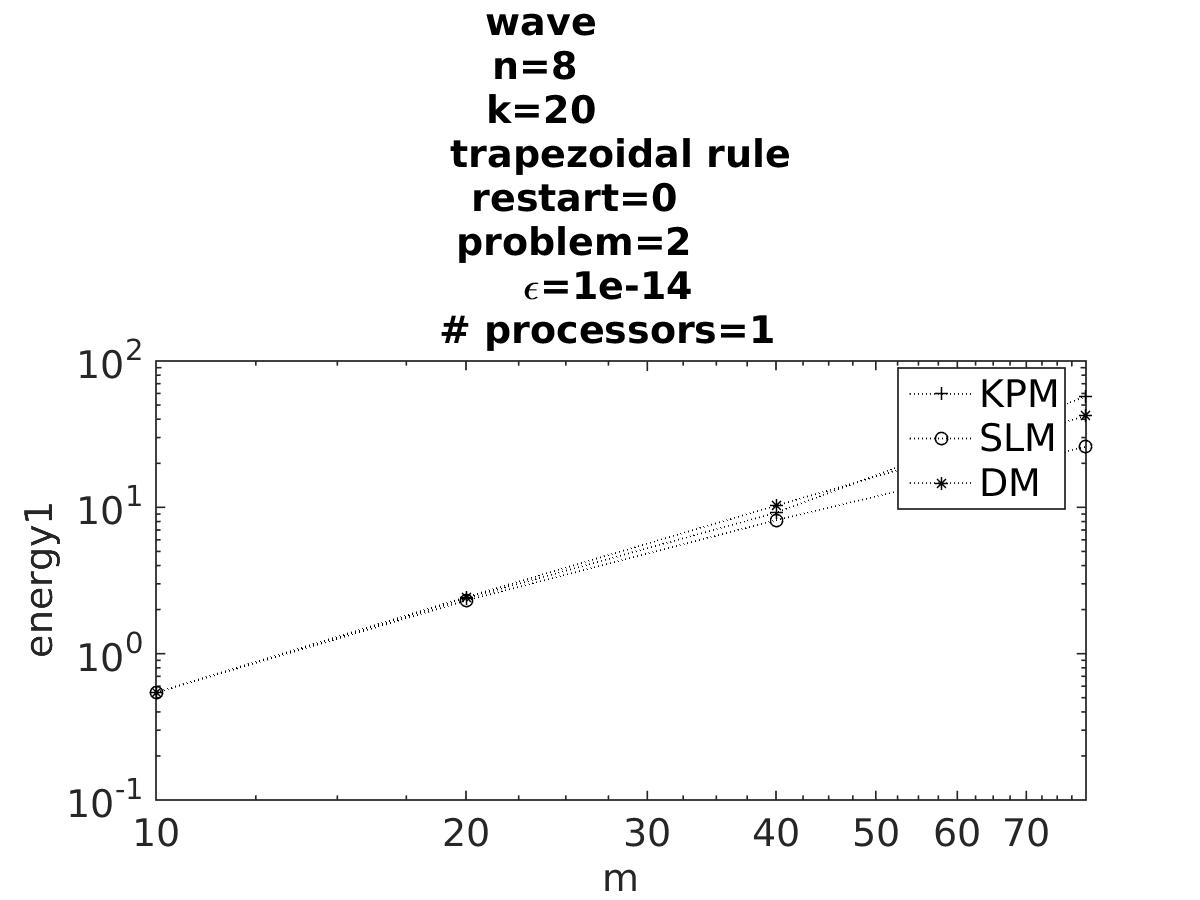
\includegraphics[width=\textwidth]{../MATLAB/fig/vresultenergyr.jpg}
                \caption{  }
                \label{fig:vresultenergy1}
        \end{subfigure}
        ~
        \begin{subfigure}[b]{0.45\textwidth}
                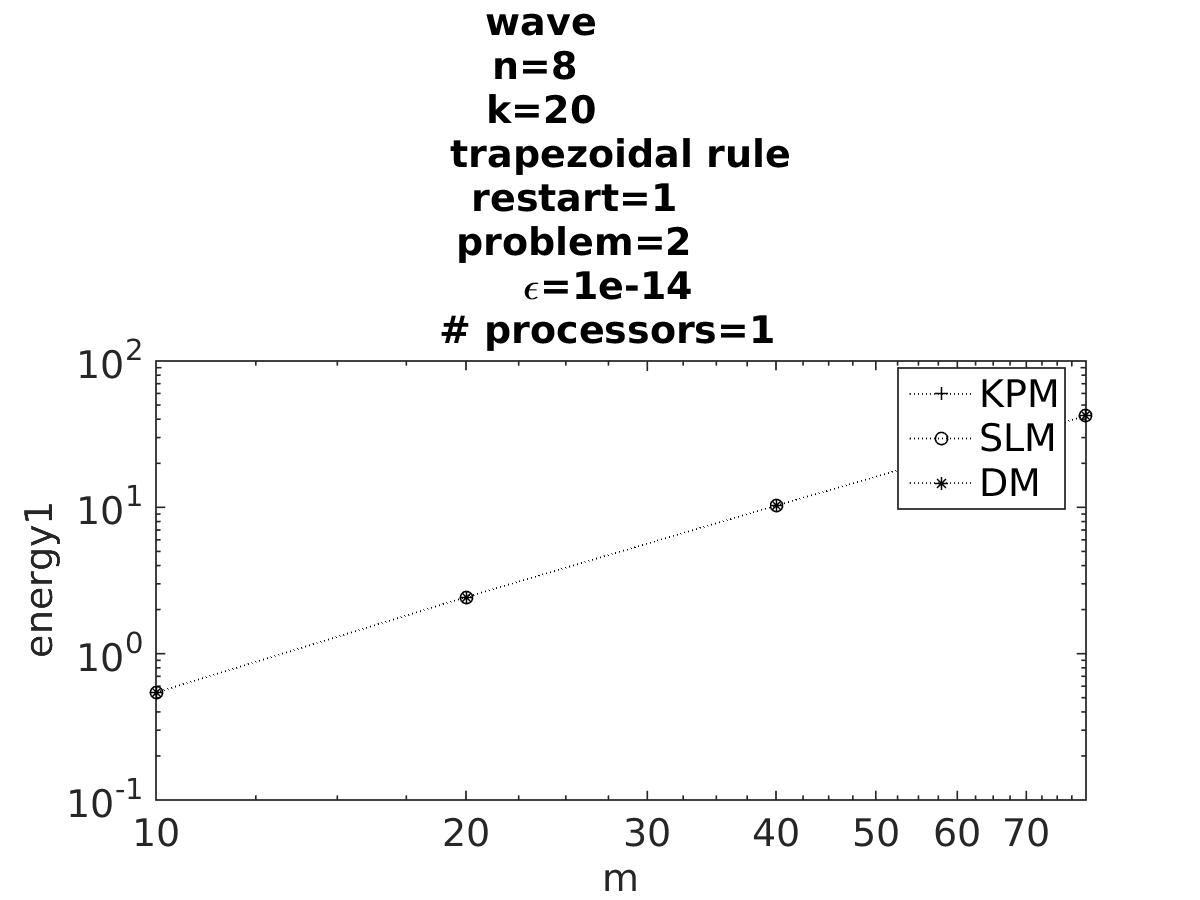
\includegraphics[width=\textwidth]{../MATLAB/fig/vresultenergy.jpg}
                \caption{  }
                \label{fig:vresultenergy2}
        \end{subfigure}
        \caption{ SLM and KPM has the best energy estimation, with DM not far behind. }
        \label{fig:vresultenergy}
\end{figure}

\section{Varying energy with the semirandom equation}
%%%%%%%%%%%%%%%%%%%%%%%%%%%%%%%%%%%%%%%%%%%%%%%%%%%%%%%%%%%%%%%%%%%%%%%%%%%%%%%%%%%%%%%%%%%%%%%%%%%%%%%

\begin{figure}[H]
        \centering
        \begin{subfigure}[b]{0.45\textwidth}
                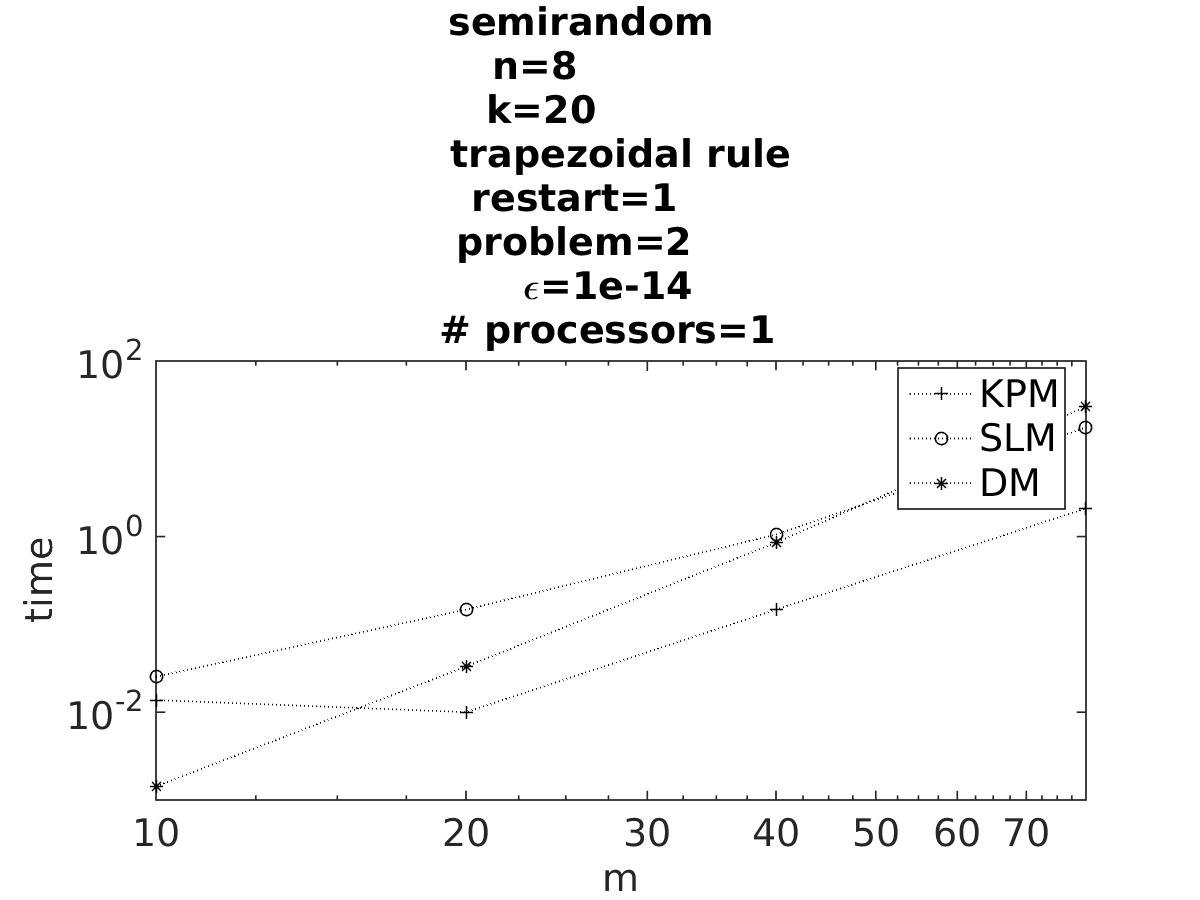
\includegraphics[width=\textwidth]{../MATLAB/fig/vsresulttimem.jpg}
                \caption{  }
                \label{fig:vsresulttimem}
        \end{subfigure}
        ~
        \begin{subfigure}[b]{0.45\textwidth}
                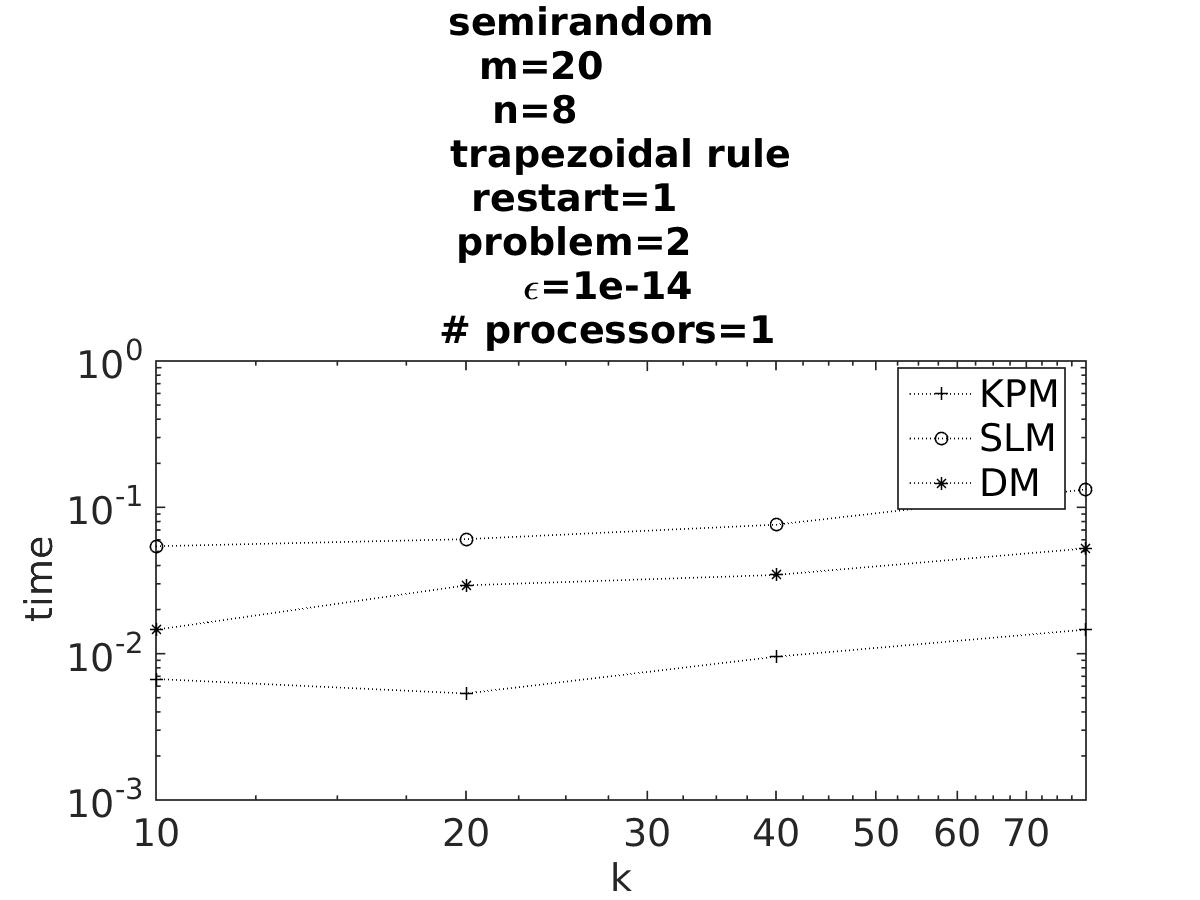
\includegraphics[width=\textwidth]{../MATLAB/fig/vsresulttimek.jpg}
                \caption{  }
                \label{fig:vsresulttimek}
        \end{subfigure}
        \caption{ For both cases KPM is faster than the other, and with DM faster than SLM.  }
        \label{fig:vsresulttime}
\end{figure}



\begin{figure}[H]
        \centering

                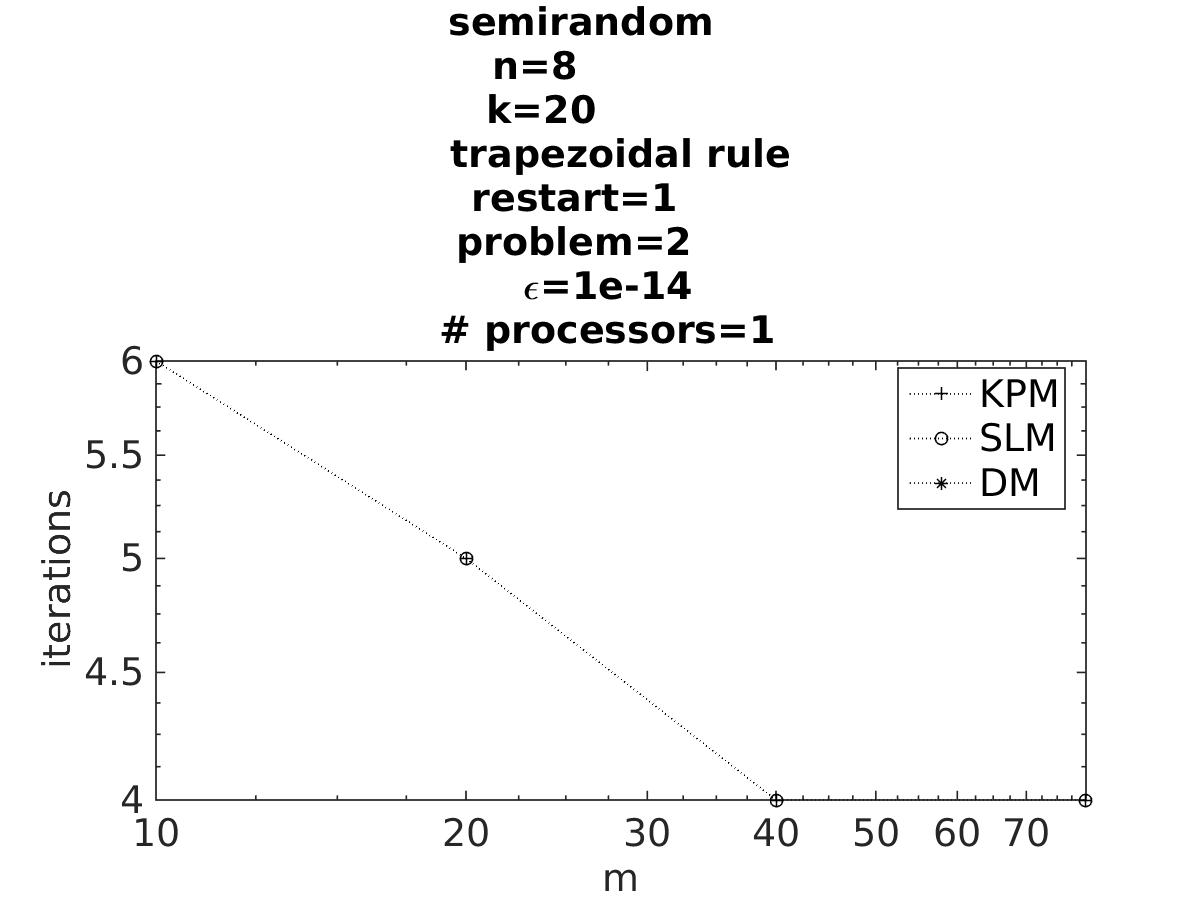
\includegraphics[width=0.45\textwidth]{../MATLAB/fig/vsresultiter.jpg}
        \label{fig:vsresultiter}
        \caption{The number of iterations are almost equal for the two methods.}
\end{figure}

\begin{figure}[H]
        \centering
        \begin{subfigure}[b]{0.45\textwidth}
                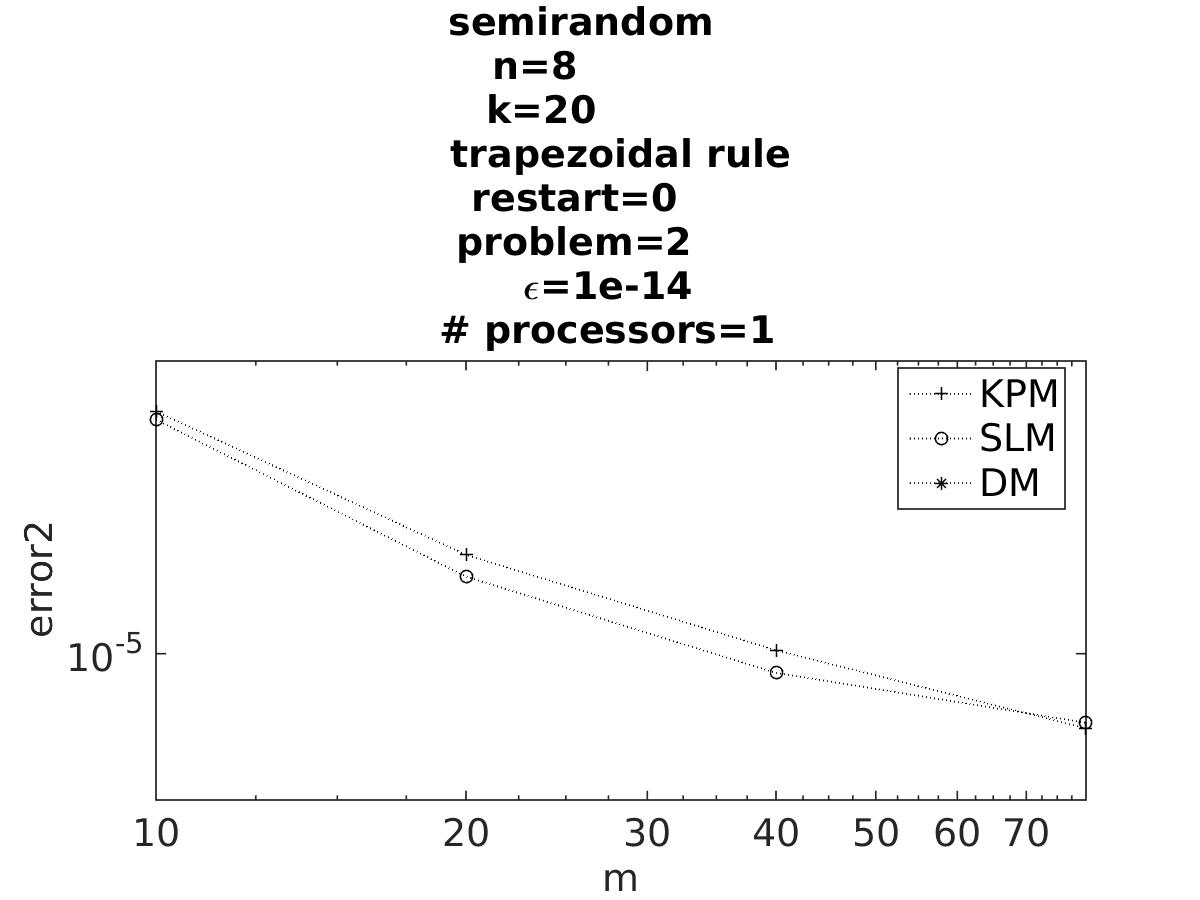
\includegraphics[width=\textwidth]{../MATLAB/fig/vsresulterrorr.jpg}
                \caption{  }
                \label{fig:vsresulterror1}
        \end{subfigure}
        ~
        \begin{subfigure}[b]{0.45\textwidth}
                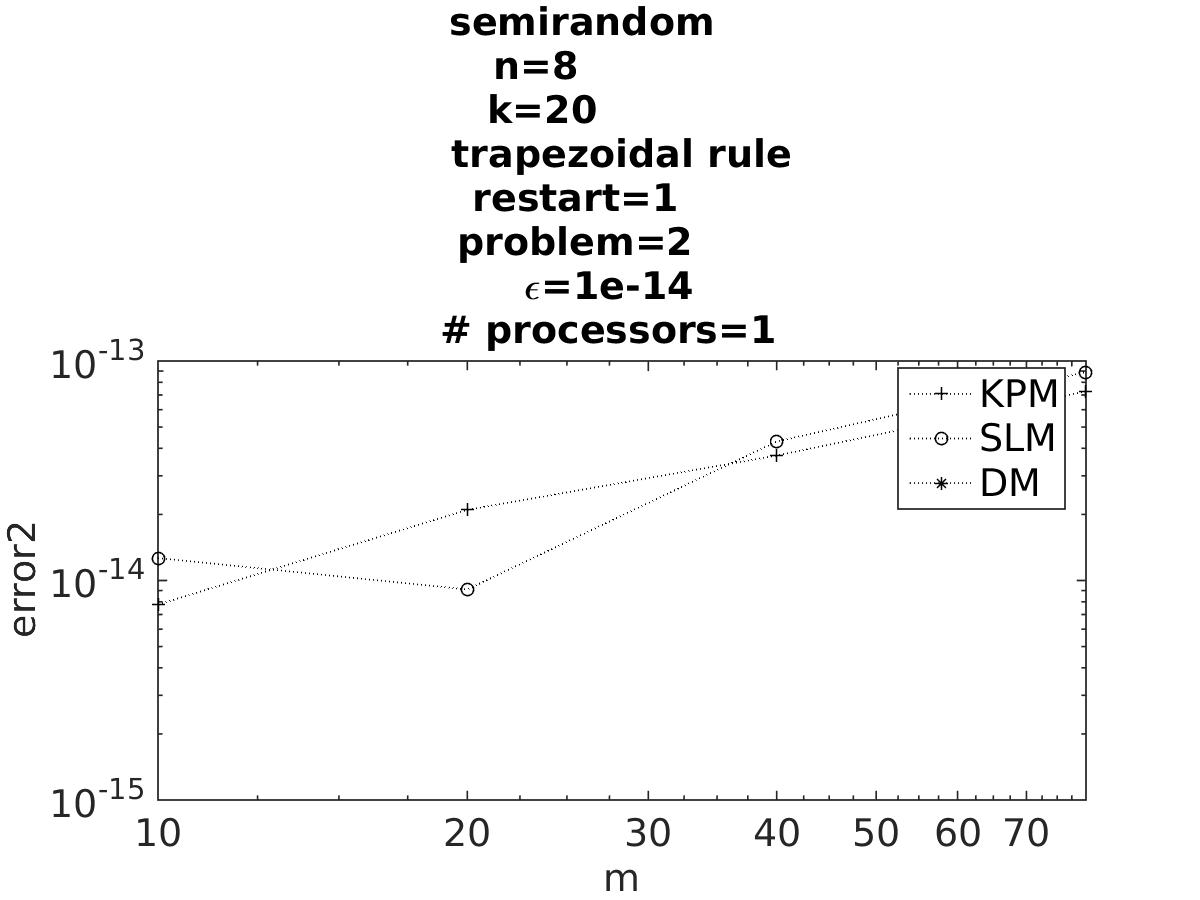
\includegraphics[width=\textwidth]{../MATLAB/fig/vsresulterror.jpg}
                \caption{  }
                \label{fig:vsresulterror2}
        \end{subfigure}
        \caption{ The error is nearly identical.  }
        \label{fig:vsresulterror}
\end{figure}


\begin{figure}[H]
        \centering
        \begin{subfigure}[b]{0.45\textwidth}
                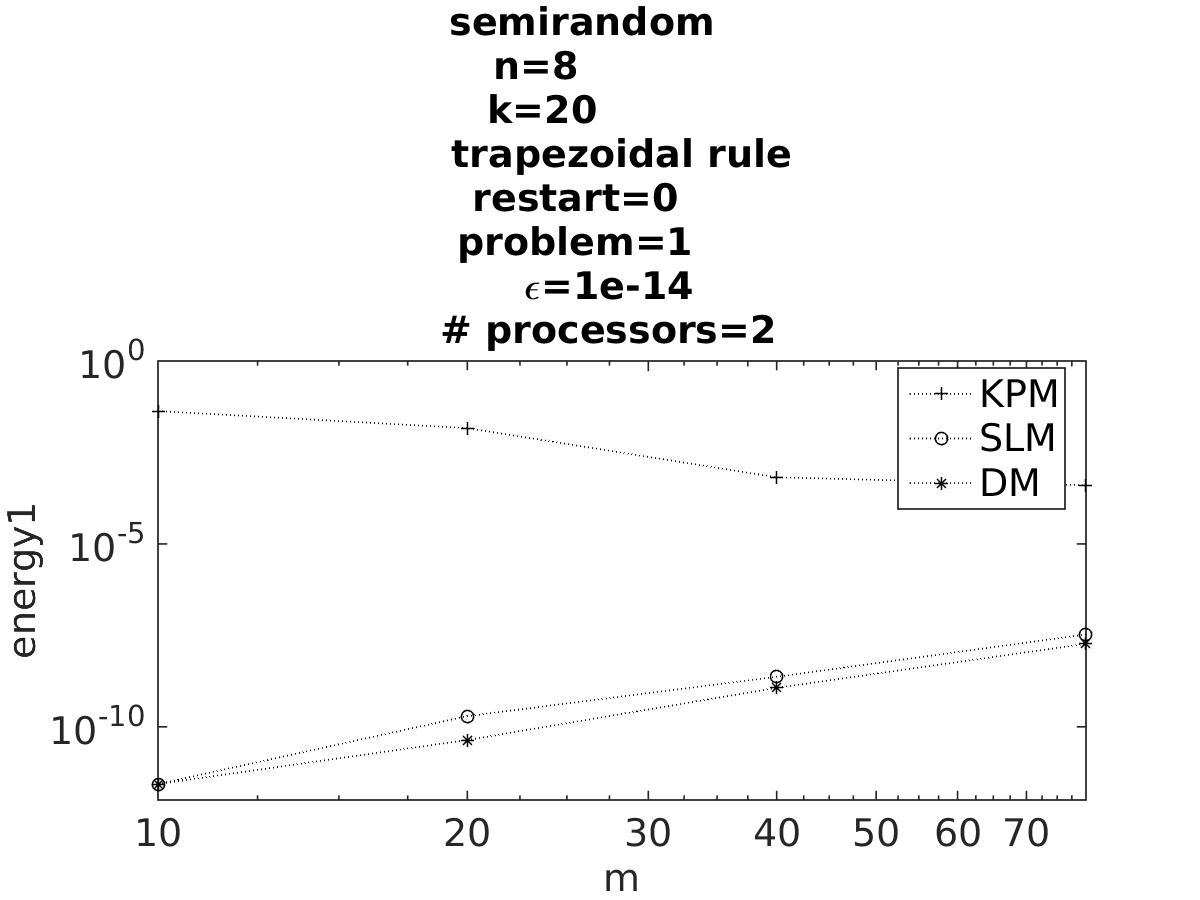
\includegraphics[width=\textwidth]{../MATLAB/fig/vsresultenergyr.jpg}
                \caption{  }
                \label{fig:vsresultenergy1}
        \end{subfigure}
        ~
        \begin{subfigure}[b]{0.45\textwidth}
                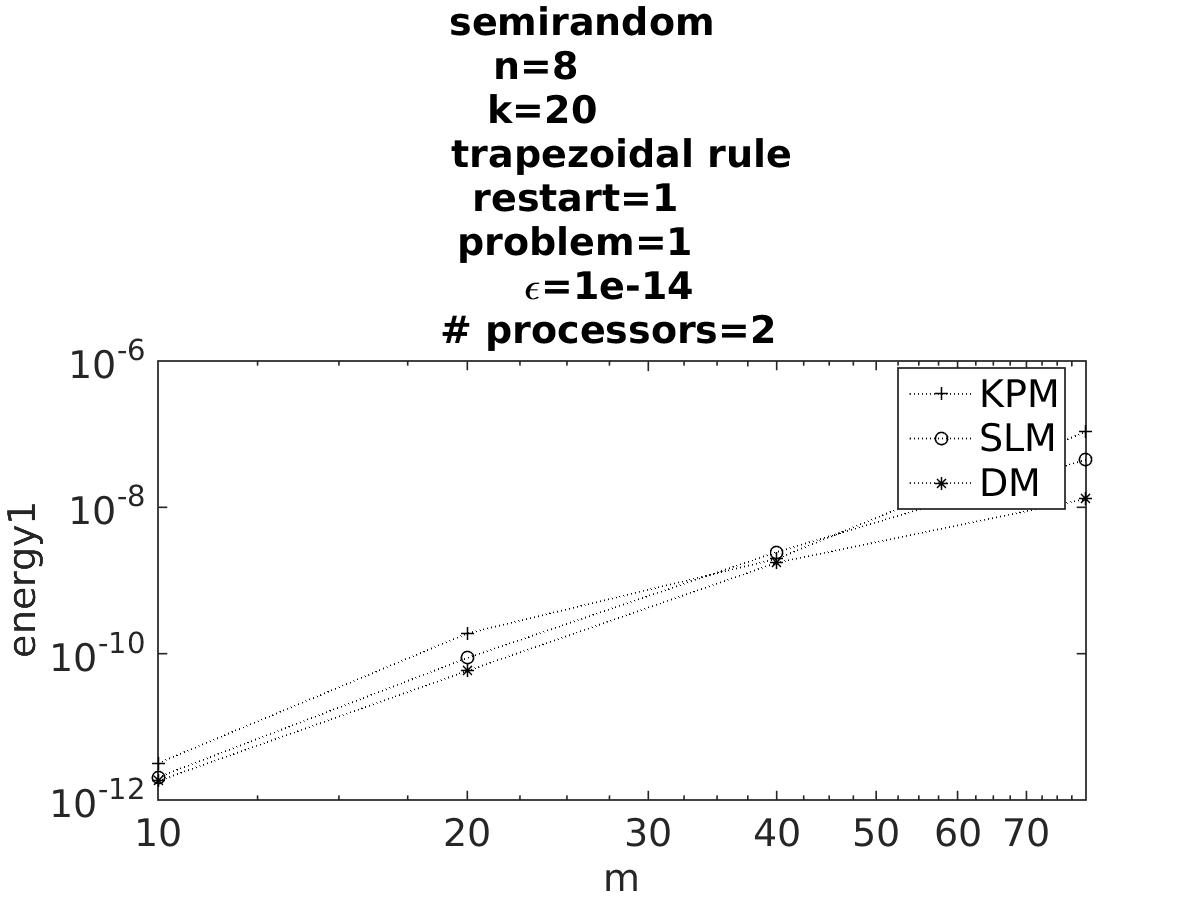
\includegraphics[width=\textwidth]{../MATLAB/fig/vsresultenergy.jpg}
                \caption{  }
                \label{fig:vsresultenergy2}
        \end{subfigure}
        \caption{ SLM and KPM has the best energy estimation, with DM not far behind. }
        \label{fig:vsresultenergy}
\end{figure}
%%%%%%%%%%%%%%%%%%%%%%%%%%%%%%%%%%%%%%%%%%%%%%%%%%%%%%%%%%%%%%%%%%%%%%%%%%%%%%%%%%%%%%%%%%%%%%%%%%%%%%%%%%%%%%%%%%%%%%%
\chapter{Results for separable $p$} \label{sec:seri}%%%%%%%%%%%%%%%%%%%%%%%%%%%%%%%%%%%%%%%%%%%%%%%%%%%%%%%%%%%%%%%%%%%%%%
%%%%%%%%%%%%%%%%%%%%%%%%%%%%%%%%%%%%%%%%%%%%%%%%%%%%%%%%%%%%%%%%%%%%%%%%%%%%%%%%%%%%%%%%%%%%%%%%%%%%%%%%%%%%%%%%%%%%%%
In this whole section it is assume that $p$ is separable, and that only one processing unit is used to obtain the results. 
Section \ref{sec:sconv} will show correctness of the methods with a convergence plot. In section \ref{sec:rrest} we will see if there is any correlation between $n$ and $\rho$.
Computation times for the different methods will be compared to each other and their predicted computational complexity in section \ref{sec:stimem} and \ref{sec:stimek}.
How $\gamma$ and $\epsilon$ scales with $\delta$ will be examined in section \ref{sec:div}.
%%%%%%%%%%%%%%%%%%%%%%%%%%%%%%%%%%%%%%%%%%%%%%%%%%%%%%%%%%%%%%%%%%%%%%%%%%%%%%%%%%%%%%%%%%%%%%%%%%%%%%%%%%%%%%%%%%%%%%
\section{Convergence} \label{sec:sconv}
%%%%%%%%%%%%%%%%%%%%%%%%%%%%%%%%%%%%%%%%%%%%%%%%%%%%%%%%%%%%%%%%%%%%%%%%%%%%%%%%%%%%%%%%%%%%%%%%%%%%%%%%%%%%%%%%%%%%%%
\begin{figure}[H]
        \centering
        \begin{subfigure}[b]{0.45\textwidth}
                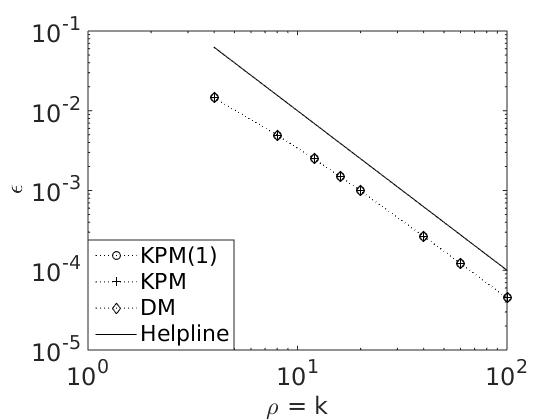
\includegraphics[width=\textwidth]{fig/s1conv1}
                \caption{function \texttt{P1}}
                \label{fig:conv1}
        \end{subfigure}%
~
        \begin{subfigure}[b]{0.45\textwidth}
                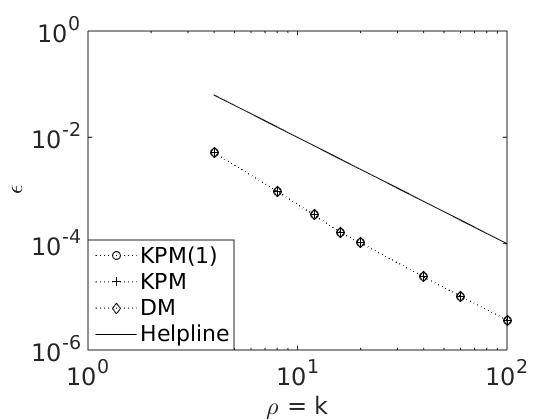
\includegraphics[width=\textwidth]{fig/s2conv2}
                \caption{function \texttt{P2}}
                \label{fig:conv2}
        \end{subfigure}
        \caption{A convergence plot for several methods with $\rho = k$. The helpline shows quadratic convergence.}\label{fig:conv}
\end{figure}
As can be seen from figure \ref{fig:conv}, all method converges quadratically and overlap perfectly, this shows that all method preforms as expected regarding convergence.
%%%%%%%%%%%%%%%%%%%%%%%%%%%%%%%%%%%%%%%%%%%%%%%%%%%%%%%%%%%%%%%%%%%%%%%%%%%%%%%%%%%%%%%%%%%%%%%%%%%%%%%%%%%%%%%%%%%%%%
\section{Choosing restart variable } \label{sec:restvar}
%%%%%%%%%%%%%%%%%%%%%%%%%%%%%%%%%%%%%%%%%%%%%%%%%%%%%%%%%%%%%%%%%%%%%%%%%%%%%%%%%%%%%%%%%%%%%%%%%%%%%%%%%%%%%%%%%%%%%%
\begin{figure}[H]
        \centering
        \begin{subfigure}[b]{0.45\textwidth}
                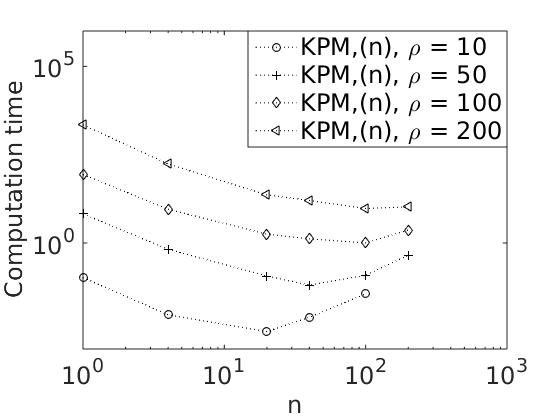
\includegraphics[width=\textwidth]{fig/s9rest1}
                \caption{function \texttt{P1}}
                \label{fig:rest1}
        \end{subfigure}
~
        \begin{subfigure}[b]{0.45\textwidth}
                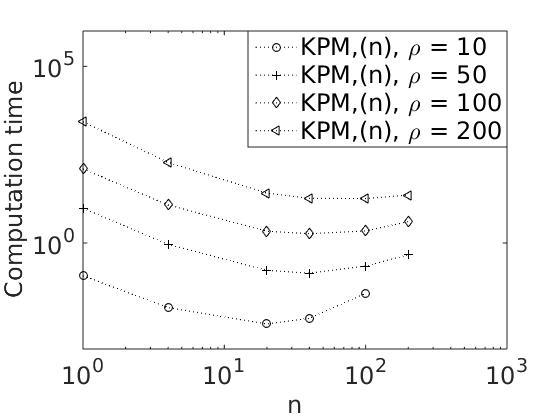
\includegraphics[width=\textwidth]{fig/s10rest2}
                \caption{function \texttt{P2}}
                \label{fig:rest2}
        \end{subfigure}
        \caption{Computation time plotted against restart variable $n$.}\label{fig:rest}
\end{figure}
As can be see from figure \ref{fig:rest}, the optimal restart variable changes as a function of $\rho$ so that larger $\rho$ needs larger $n$ to preform optimally, $n = \rho$ seams to give the smallest computation time for the cases tested. One point is missing from \texttt{KPM}$(n)$, $\rho = 10$, this is because the last point plotted is the same as \texttt{KPM}.  
%%%%%%%%%%%%%%%%%%%%%%%%%%%%%%%%%%%%%%%%%%%%%%%%%%%%%%%%%%%%%%%%%%%%%%%%%%%%%%%%%%%%%%%%%%%%%%%%%%%%%%%%%%%%%%%%%%%%%%
\section{Comparing $\gamma$ and $n$} \label{sec:rrest}
%%%%%%%%%%%%%%%%%%%%%%%%%%%%%%%%%%%%%%%%%%%%%%%%%%%%%%%%%%%%%%%%%%%%%%%%%%%%%%%%%%%%%%%%%%%%%%%%%%%%%%%%%%%%%%%%%%%%%%
\begin{figure}[H]
        \centering
        \begin{subfigure}[b]{0.45\textwidth}
                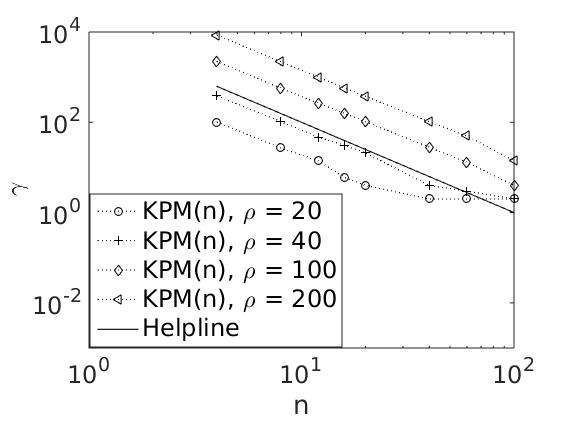
\includegraphics[width=\textwidth]{fig/s3antvsm1}
                \caption{function \texttt{P1}}
                \label{fig:ant1}
        \end{subfigure}%
~
        \begin{subfigure}[b]{0.45\textwidth}
                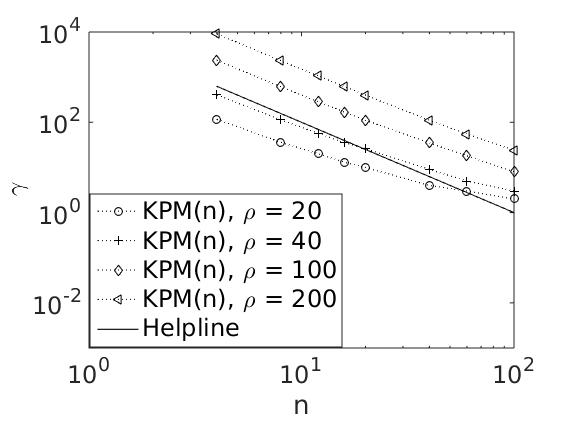
\includegraphics[width=\textwidth]{fig/s4antvsm2}
                \caption{function \texttt{P2}}
                \label{fig:ant2}
        \end{subfigure}
        \caption{The number of restarts, $\gamma$ needed for \texttt{KPM}$(n)$ to converge as a function of the restart variable $n$. The helpline follows $1/n^2$.}\label{fig:ant}
\end{figure}

The helpline from figure \ref{fig:ant} shows that the number of restarts is proportional to $1/n^2$ for all tested cases, if we put this together with the assumption from section \ref{sec:cc} we get that $\gamma$ is proportional to  $m^2/n^2$. Using table \ref{tab:cc} we get that \texttt{KPM}$(n)$ has a complexity of $\mathcal{O}(km^2 + m^3)$ for separable $p$, and $\mathcal{O}(km^3 + m^4)$ for non-separable $p$, which is the same as for \texttt{KPM}.\\

We also see that the number of restarts decrease quickest when $n < \rho $, and slower when $n > \rho$. This is the gain we observed in section \ref{sec:restvar}. On each side of $n = \rho$ we can perform better, either by performing fewer restarts with larger matrices, or more restarts with smaller matrices. \\
%%%%%%%%%%%%%%%%%%%%%%%%%%%%%%%%%%%%%%%%%%%%%%%%%%%%%%%%%%%%%%%%%%%%%%%%%%%%%%%%%%%%%%%%%%%%%%%%%%%%%%%%%%%%%%%%%%%%%%
\section{Computation time with different $\rho$} \label{sec:stimem}
%%%%%%%%%%%%%%%%%%%%%%%%%%%%%%%%%%%%%%%%%%%%%%%%%%%%%%%%%%%%%%%%%%%%%%%%%%%%%%%%%%%%%%%%%%%%%%%%%%%%%%%%%%%%%%%%%%%%%%
\begin{figure}[H]
        \centering
        \begin{subfigure}[b]{0.45\textwidth}
                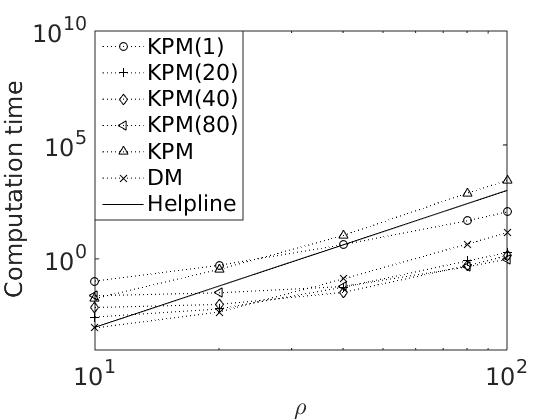
\includegraphics[width=\textwidth]{fig/n5timevsm1}
                \caption{function \texttt{P1}}
                \label{fig:timem1}
        \end{subfigure}%
        ~
        \begin{subfigure}[b]{0.45\textwidth}
                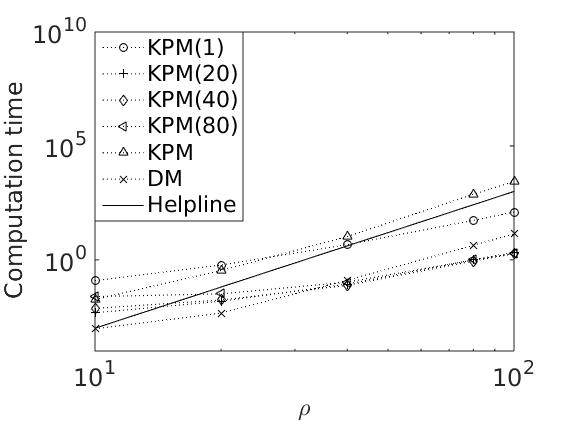
\includegraphics[width=\textwidth]{fig/n6timevsm2}
                \caption{function \texttt{P2}}
                \label{fig:timem2}
        \end{subfigure}
        \caption{A plot of computation time as a function of $\rho$. The helpline increases with $\rho^6 = m^3$.}\label{fig:timem}
\end{figure}
As we can see from figure \ref{fig:timem}, the computation time for \texttt{KPM} increases as expected, while \texttt{DM} and \texttt{KPM}$(n)$ increases slower, perhaps due to MATLAB's efficient inversion algorithm or less memory demand. 
Even more interesting is it that \texttt{KPM}$(n)$ is both asymptotically better, and faster than \texttt{DM} for large $\rho$. Clearly \texttt{KPM}$(n)$ is better in some cases.
%%%%%%%%%%%%%%%%%%%%%%%%%%%%%%%%%%%%%%%%%%%%%%%%%%%%%%%%%%%%%%%%%%%%%%%%%%%%%%%%%%%%%%%%%%%%%%%%%%%%%%%%%%%%%%%%%%%%%%
\section{Computation time with different $k$} \label{sec:stimek}
%%%%%%%%%%%%%%%%%%%%%%%%%%%%%%%%%%%%%%%%%%%%%%%%%%%%%%%%%%%%%%%%%%%%%%%%%%%%%%%%%%%%%%%%%%%%%%%%%%%%%%%%%%%%%%%%%%%%%%
\begin{figure}[H]
        \centering
        \begin{subfigure}[b]{0.45\textwidth}
                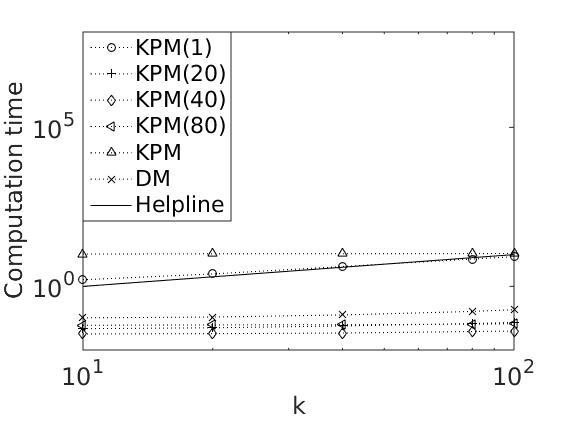
\includegraphics[width=\textwidth]{fig/n7timevsk1}
                \caption{function \texttt{P1}}
                \label{fig:timek1}
        \end{subfigure}%
~
        \begin{subfigure}[b]{0.45\textwidth}
                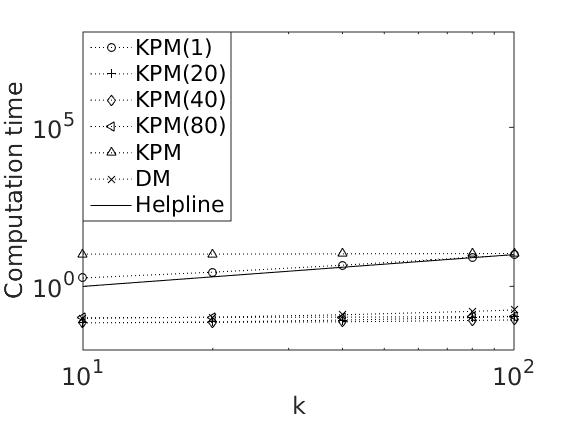
\includegraphics[width=\textwidth]{fig/n8timevsk2}
                \caption{function \texttt{P2}}
                \label{fig:timek2}
        \end{subfigure}
        \caption{A plot of computation time as a function of $k$. The helpline increases with $k$.}\label{fig:timek}
\end{figure}
As we can see from figure \ref{fig:timek}, the computation time for almost all tested methods are constant. The reason is that the time needed for initializing is much greater than the time it takes to integrate. 
The exception is \texttt{KPM}$(1)$, which increases close to linear because relatively more work is done while integrating, due to several restarts. 
We also see that \texttt{KPM}$(n)$ is faster than \texttt{DM} for some $n$, but not asymptotically.

With larger $k$ it is expected that all methods would follow the helpline.
%%%%%%%%%%%%%%%%%%%%%%%%%%%%%%%%%%%%%%%%%%%%%%%%%%%%%%%%%%%%%%%%%%%%%%%%%%%%%%%%%%%%%%%%%%%%%%%%%%%%%%%%%%%%%%%%%%%%%%
\section{Comparing $\delta$, $\gamma$ and $\epsilon$ } \label{sec:div}
%%%%%%%%%%%%%%%%%%%%%%%%%%%%%%%%%%%%%%%%%%%%%%%%%%%%%%%%%%%%%%%%%%%%%%%%%%%%%%%%%%%%%%%%%%%%%%%%%%%%%%%%%%%%%%%%%%%%%%
Remember that $\delta$ is tolerance, $\gamma$ is the number of restarts, and $\epsilon$ is a measure for the error.
\begin{figure}[H]
        \centering
        \begin{subfigure}[b]{0.45\textwidth}
                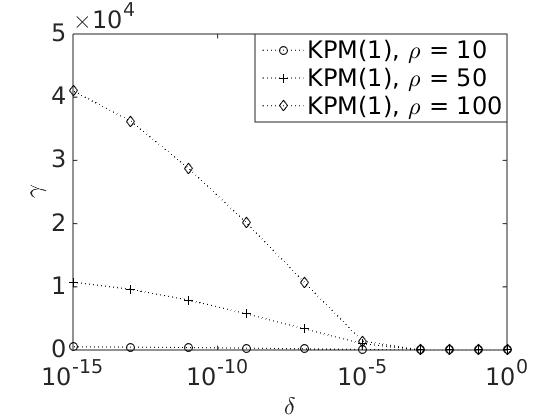
\includegraphics[width=\textwidth]{fig/s13antvstol1m}
                \caption{function \texttt{P1}}
                \label{fig:gammadelta1}
        \end{subfigure}
~
        \begin{subfigure}[b]{0.45\textwidth}
                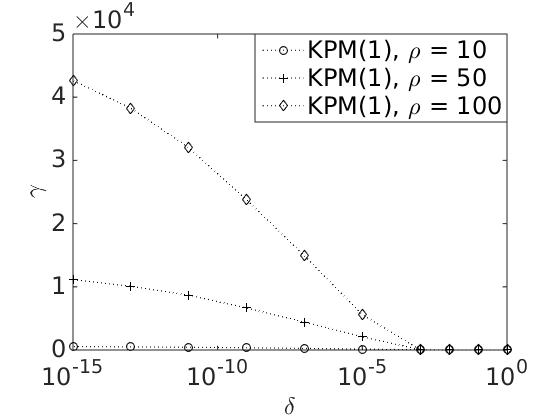
\includegraphics[width=\textwidth]{fig/s14antvstol2m}
                \caption{ function \texttt{P2}}
                \label{fig:gammadelta2}
        \end{subfigure}
        
        \begin{subfigure}[b]{0.45\textwidth}
                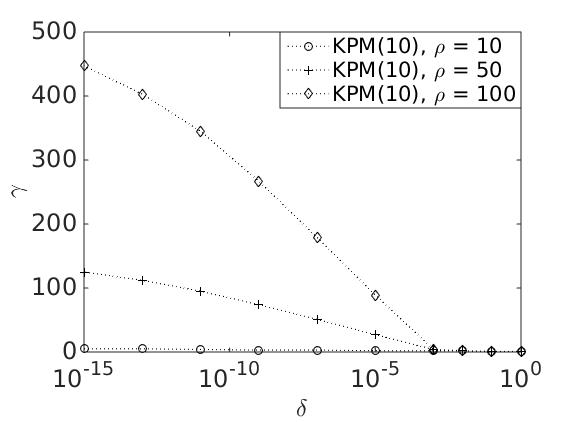
\includegraphics[width=\textwidth]{fig/s13antvstol1m10}
                \caption{function \texttt{P1}}
                \label{fig:gammadelta3}
        \end{subfigure}
~
        \begin{subfigure}[b]{0.45\textwidth}
                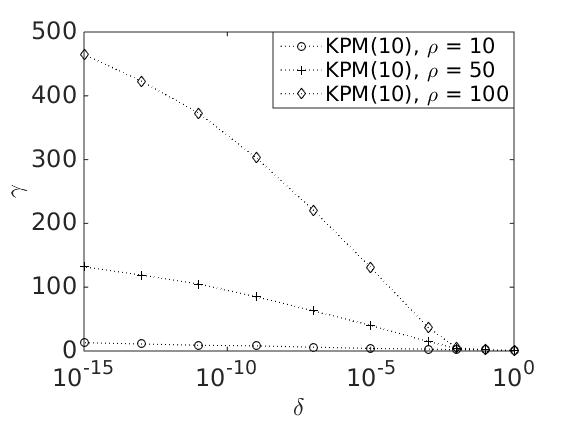
\includegraphics[width=\textwidth]{fig/s14antvstol2m10}
                \caption{ function \texttt{P2}}
                \label{fig:gammadelta4}
        \end{subfigure}
        
        \caption{A plot of $\gamma$ as a function of $\delta$, with several $\rho$ and $n$.} \label{fig:gammadelta}
\end{figure}
%We see from figure \ref{fig:gammadelta} that $\gamma$ changes significantly with $\rho$. The figure show a log linear dependence between $\gamma$ and $\delta$, and that $\gamma$ is proportional to $1/n^2$. 

We see from figure \ref{fig:gammadelta} that $\gamma$ changes significantly with $\rho$, that there is a log linear dependence between $\gamma$ and $\delta$, and that $\gamma$ is proportional to $1/n^2$. 

The constant part of the graph where $ 10^{-5}<\delta< {10^0} $ shows that \texttt{KPM}$(1)$ and \texttt{KPM}$(10)$ does too few restarts to gain any accuracy when $\delta$ is too large, this is confirmed by figure \ref{fig:epsilondelta}. 

\begin{figure}[H]
        \centering
        \begin{subfigure}[b]{0.45\textwidth}
                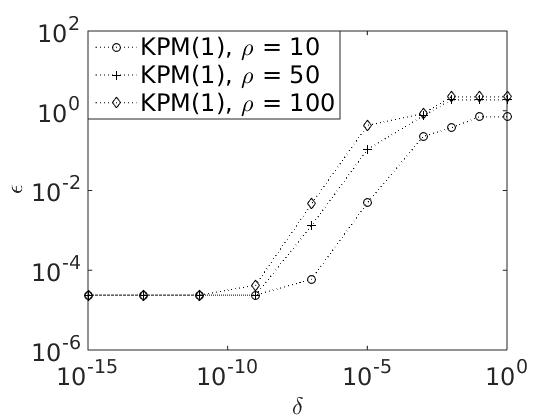
\includegraphics[width=\textwidth]{fig/s15errvstol1m}
                \caption{function \texttt{P1}}
                \label{fig:epsilondelta1}
        \end{subfigure}
~
        \begin{subfigure}[b]{0.45\textwidth}
                \includegraphics[width=\textwidth]{fig/s16errvstol2m}
                \caption{ function \texttt{P2}}
                \label{fig:epsilondelta2}
        \end{subfigure}
        
        \begin{subfigure}[b]{0.45\textwidth}
                \includegraphics[width=\textwidth]{fig/s15errvstol1m10}
                \caption{function \texttt{P1}}
                \label{fig:epsilondelta3}
        \end{subfigure}
~
        \begin{subfigure}[b]{0.45\textwidth}
                \includegraphics[width=\textwidth]{fig/s16errvstol2m10}
                \caption{ function \texttt{P2}}
                \label{fig:epsilondelta4}
        \end{subfigure}
        
        \caption{A plot of $\epsilon$ as a function of $\delta$, with several $\rho$ and $n$.} \label{fig:epsilondelta}
\end{figure}
Figure \ref{fig:epsilondelta} shows $\epsilon$ as a function of $\delta$. In figure \ref{fig:epsilondelta1} and \ref{fig:epsilondelta3} all graphs has obtained the threshold precision possible with $k=40$. In
figure \ref{fig:epsilondelta2} and \ref{fig:epsilondelta4} the precision possible with the different $\rho$-s are obtained. It seams that the maximum precision is attained faster with larger $n$, this makes sense because if $n = m$, we should not need to restart in order to get threshold precision. This was also confirmed by figure \ref{fig:gammadelta}, where \texttt{KPM}$(10)$ needed fewer restarts than \texttt{KPM}$(1)$ to converge. 
%There is no reason this was not performed with other than $n = 1$ except for laziness. \\
%!!!!!!!!!!!!!!!!!!!!!!!!!Arg, jeg må lage nye figurer for andre $n$!!!!!!!!!!!!!!!!!!!!!!!!!!!!!!!!!!\\
%!!!!!!!!!!!!!!!!Her kan burde skrive noe om hvor bra KPM$(n)$ uten restart ville vært!!!!!!!!!!!!!!!!\\
%!!!!!!!!!!!!!!!!!!!!!Fjern alle forekomster av ordet "shows" fra avsnittet!!!!!!!!!!!!!!!!!!!!!!!!!!!!\\
%!!!!!!!!!!!!!!!!!!!!!Forklare hva alle variablene er over alt!!!!!!!!!!!!!!!!!!!!!!!!!!\\
%!!!!!!!!!!!!!!!!!!!!!Skrive hvorfor vi ikke har med noe annet enn KPM$(1)$!!!!!!!!!!!!!!!!!!\\
%!!!!!!!!!!!!!!!!!!!!!!!!!!!Går videre så jeg ikke trenger å lage nye figurer med en gang!!!!!!!!!!!!!!!!!!!!!!!!!!\\
%Figure \ref{fig:errant} and \ref{fig:errtolk} shows how $\gamma$ and $\epsilon$ scales with $\delta$. Figure \ref{fig:errtol1} has reached to threshold precision with $k = 40$. Both figures shows a loglinear dependence between $\gamma$ and $\delta$. The figures also shows the importance of choosing an appropriate $\delta$. A lot of time can be saved by choosing $\delta$ larger, but precision is lost if $\delta$ is to large.
\begin{figure}[H]
        \centering
        \begin{subfigure}[b]{0.45\textwidth}
                \includegraphics[width=\textwidth]{fig/s20antvstol1k}
                \caption{function \texttt{P1}}
                \label{fig:gammadeltak1}
        \end{subfigure}
~
        \begin{subfigure}[b]{0.45\textwidth}
                \includegraphics[width=\textwidth]{fig/s21antvstol2k}
                \caption{ function \texttt{P2}}
                \label{fig:gammadeltak2}
        \end{subfigure}
                \begin{subfigure}[b]{0.45\textwidth}
                \includegraphics[width=\textwidth]{fig/s20antvstol1k10}
                \caption{function \texttt{P1}}
                \label{fig:gammadeltak3}
        \end{subfigure}
~
        \begin{subfigure}[b]{0.45\textwidth}
                \includegraphics[width=\textwidth]{fig/s21antvstol2k10}
                \caption{ function \texttt{P2}}
                \label{fig:gammadeltak4}
        \end{subfigure}
        \caption{A plot of $\gamma$ as a function of $\delta$, with several $k$ and $n$.} \label{fig:gammadeltak}
\end{figure}
Figure \ref{fig:gammadeltak} shows that $\gamma$ is nearly independent of $k$. The figures also shows the log linear dependence between $\delta$ and $\gamma$. \\



\begin{figure}[H]
        \centering
        \begin{subfigure}[b]{0.45\textwidth}
                \includegraphics[width=\textwidth]{fig/s22errvstol1k}
                \caption{function \texttt{P1}}
                \label{fig:epsilondelta1k}
        \end{subfigure}
~
        \begin{subfigure}[b]{0.45\textwidth}
                \includegraphics[width=\textwidth]{fig/s23errvstol2k}
                \caption{ function \texttt{P2}}
                \label{fig:epsilondelta2k}
        \end{subfigure}
                \begin{subfigure}[b]{0.45\textwidth}
                \includegraphics[width=\textwidth]{fig/s22errvstol1k10}
                \caption{function \texttt{P1}}
                \label{fig:epsilondelta3k}
        \end{subfigure}
~
        \begin{subfigure}[b]{0.45\textwidth}
                \includegraphics[width=\textwidth]{fig/s23errvstol2k10}
                \caption{ function \texttt{P2}}
                \label{fig:epsilondelta4k}
        \end{subfigure}
        \caption{A plot of $\epsilon$ as a function of $\delta$, with several $k$ and $n$.} \label{fig:epsilondeltak}
\end{figure}
Figure \ref{fig:epsilondeltak} shows much the same as figure \ref{fig:epsilondelta}. Maximum precision for different $k$-s are shown in figure \ref{fig:epsilondelta1k} and \ref{fig:epsilondelta3k}.
Threshold precision for $\rho = 40$ is obtained in figure \ref{fig:epsilondelta2k} and \ref{fig:epsilondelta4k}, but not for the graph where $k = 10$, this is the precision possible with $k=10$. Again $\epsilon$ converges faster for \texttt{KPM}$(10)$ than \texttt{KPM}$(1)$. \\

We see that there is no gain in precision with increasing one of either $\rho$ or $k$ or decreasing $\delta$ without changing the others appropriately. \\

%Before the constant part, $\epsilon$ is decided by $\delta$ alone. 
In all cases a lot of time can be saved by choosing $\delta$ appropriate. If $\delta$ is to large we get inaccurate answers, if $\delta$ is to small we perform to many restarts to use the algorithm efficiently. There does not seam to be a simple rule to choose $\delta$, since the results for \texttt{P1} and \texttt{P2} differs. The rule we will use is to start at $\delta=10^{-3}$ with $\rho = k = 10$, and decrease $\delta$ with one order of magnitude each time $k$ and $\rho$ is doubled. %The reason for this rule is perhaps easier to understand when looking at figure \ref{fig:conv}. %The reason that $\delta$ decreases two orders of magnitude each time $m$ and $k$ is doubled is that $A$ and trapezoidal rule are second order approximations. 
Figure \ref{fig:siste} shows how the error converges when this is the case. It is clear that that this rule should depend on the problem. For \texttt{P1}  the initial $\delta$ should be chosen a little smaller, for \texttt{P2} $\delta$ should decrease a little quicker, perhaps with 1.1 order of magnitude. This rule gives a little loss in accuracy, but a great increase in performance. Notice that the convergence is still quadratic.

\begin{figure}[H]
        \centering
        \begin{subfigure}[b]{0.45\textwidth}
                \includegraphics[width=\textwidth]{fig/sisteplot1}
                \caption{function \texttt{P1}}
                \label{fig:siste1}
        \end{subfigure}
~
        \begin{subfigure}[b]{0.45\textwidth}
                \includegraphics[width=\textwidth]{fig/sisteplot2}
                \caption{ function \texttt{P2}}
                \label{fig:siste2}
        \end{subfigure}
        \caption{A plot of $\epsilon$ where $\delta$, $k$, $\rho$ and $n$ follows this rule: Start with $\delta=10^{-3}$, $\rho = k = n = 10$ and decrease $\delta$ with one order of magnitude each time $k$, $\rho$ and $n$ is doubled. \texttt{DM} Shows how it converged when $\delta = 10^{-15}$. The helpline shows quadratic convergence.} \label{fig:siste}
\end{figure}


%\chapter{ Conclusion }
%The conclusion is, for simplicity, divided in the same two cases that the results were divided into. \\
%The goals with this thesis was to see how the error and energy for the Krylov methods compared 

\noindent The aim with this thesis is was to study two Krylov methods and the restart, and compare them to other popular solution methods in: 
global error, energy preservation, and computation time. The energy preservation for \texttt{SLM} was also examined, together with derivation of the methods and proof of convergence. \\

\noindent The Krylov methods have been compared to \texttt{DM} (see Section \ref{sec:DM}), in error, energy and computation time. Two different Hamiltonian ODEs were used, one was random (See Section \ref{sec:random}), and the other was a discretization of the wave equation (See Section \ref{sec:wave}). Two very different cases were also tested: constant energy, and varying energy. These cases were handled differently. In the case with constant energy, the error was measured with an exact solver, see Table \ref{tab:intcorrect}. When the energy was varying, both error and energy was measured against \texttt{DM}. Because of this, the conclusion is divided into two parts, Section \ref{sec:Konkconst} and \ref{sec:Konkvari}. \\

\noindent The wave equation gave nice results for any $n$, which made the restart uninteresting. To better show how the restarts can be used to improve the solution, only the random test case was used. If you want to use a Krylov method to solve the wave equation, this is very efficient.

\section{Constant energy} %%%%%%%%%%%%%%%%%%%%%%%%%%%%%%%%%%%%%%%%%%%%%%%%%%%%%%%
\label{sec:Konkconst}
The restart can be effectively used to improve the error if a small restart variable (see Section \ref{sec:KPM}) is preferred (see Figure \ref{fig:lcompareErrorw}). \\

\noindent \textbf{When restart is not enabled:} The error for all methods increase linearly with time (see Figure \ref{fig:longtime2err}). \texttt{SLM} is energy preserving (see Figure \ref{fig:vlongene}). \texttt{KPM}s energy is not preserved, but it is bounded. Using an  exact solver instead of the trapezoidal rule gives a smaller error, but does not change the energy (see Figure \ref{fig:idea0}). Both \texttt{SLM} and \texttt{KPM} is faster than \texttt{DM} (see Figure \ref{fig:time0}). This makes \texttt{SLM} an excellent solver on linear Hamiltonian ODEs, when restart is not used.\\

\noindent \textbf{When restart is enabled:} \texttt{SLM} and \texttt{KPM} behave very similar. The error increases linearly with time, but diverges on long time domains (see Figure \ref{fig:SLMenergyerror0} and \ref{fig:vlong}). The energy also increases slowly with time, and diverges on long time domains. Using windowing, the performance of the methods is improved, see Section \ref{sec:windu} and Figure \ref{fig:windowingc}. Using an exact solver instead of the trapezoidal rule gives a smaller error, but does not change the energy (see Figure \ref{fig:idea0}). \texttt{SLM} is very slow, making it less useful  (see Figure \ref{fig:time0}). \texttt{KPM}, on the other hand, is quite fast, but only if the matrix is big, the number of steps in time is small, and the restart variable is well chosen (see Figure \ref{fig:timekr1}). This means that \texttt{KPM} often will be the better alternative of the two methods, when restart is used. \\

\noindent Using windowing and/or an exact solver does not change the computation time, see Figure \ref{fig:time2} and \ref{fig:time3}.
\section{Varying energy} %%%%%%%%%%%%%%%%%%%%%%%%%%%%%%%%%%%%%%%%%%%%%%%%%%%%%%%%%%
\label{sec:Konkvari}

For \texttt{SLM} and \texttt{KPM} without restart, the energy and error are bounded, but not constant (see Figure \ref{fig:vSLMenergyerror1}). When restart is enabled, the energy and error increases slower, but diverges on long time domains (see Figure \ref{fig:vSLMenergyerror0}). The divergence cannot be removed by windowing (see Figure \ref{fig:lversuskenergy}). Compared to \texttt{DM}, \texttt{SLM} is slow, while \texttt{KPM} is fast if the size of the matrix is large, the number of time steps is small, and $n$ is well chosen (see Figure \ref{fig:ltime0}). This makes \texttt{KPM} the better choice if this is the case, and \texttt{DM} better in the other cases.

\section{Further work}
It could be interesting to see how the error and energy behave with a random Hamiltonian matrix with different structures (eg. full random, sparse 5-diagonal, 1-diagonal), with a known analytical solution (eg. make an accurate eigenvalue/eigenvector decomposition of the matrix and then take the exponential of the diagonal matrix of eigenvalues, or use the method based on the shur decomposition).
This could shed more light on when and how to best utilize the Krylov methods.\\

\noindent The Krylov methods ability to create small matrices can make it possible to utilize graphics cards as the processing unit. Graphics cards are designed to be used on small matrices \cite{graphics}. They consists of thousands of processing units, which could be used to solve non linear Hamiltonian problems in parallel (see Section \ref{sec:linear}).

%\chapter{  }
\section{Code}
All code used to create results in the text can be found on github: \\
\url{https://github.com/sindreka/Master}
\section{Further work}
The implemented test problems has some limitations. It could be interesting to see how the error and energy behaved with a random Hamiltonian matrix, with a known analytical solution, specifically \texttt{expm} with restart and windowing, and the relation between $n$ and $m$. \\

Graphics cards are designed to solve small matrices in parallel \cite{graphics}. When the energy is constant windowing can be used to ensure convergence with this $n$. This could then be used to solve non linear Hamiltonian problems in parallel under optimized conditions. \\



\section{Conclusion}
%\begin{itemize}
%\item Linear error stigning
%\item Constant energy
%\item Skriv det som står her inn i resultatene også??
%\item Skroll gjennom resultatene, og så skriv paralletl med det.
%\item er SLM uten restart energi bevarende
%\item er SLM med restart energi bevarende
%\item Hvor raskt øker feilen for SLM med og uten restart.
%\item rekkefølge:
%\item Convergence
%\item convergence with $\iota$
%\item convergence with $i_r$
%
%\end{itemize}
Since the results are divided in two cases it feels natural to divide the conclusion in two case.
\subsection{Constant energy} %%%%%%%%%%%%%%%%%%%%%%%%%%%%%%%%%%%%%%%%%%%%%%%%%%%%%%%
The error for both \texttt{KPM} and \texttt{SLM} is found to increase linearly within a reasonable time domain with suitable $n$. With large time domains or small $n$ it was found a sudden increase in error. If restart is enabled the growth is unbounded and exponential, while it is bounded when restart is not enabled.\\
The sudden increase in error could be solved completely with windowing. \\
The energy for both projection methods is increasing very slowly, and about the same as for \texttt{DM}. This suggests that the increase is actually a result of rounding errors, and not a fault in the method. The energy for \texttt{SLM} is preserved if restart is not enabled, even on long time domains. \\

Because of \texttt{SLM}'s energy preserving properties it was predicted that it would massively outperform \texttt{KPM}. This has proven to only be partially true, as the error will be equally big for both projection methods. If energy preservation is important \texttt{SLM} can achieve this with a fairly small matrix. If a small error is necessary there are two ways this can be done, either with restart, or with a larger $n$. If restart is used \texttt{SLM} looses its energy preserving property, and behaves very similar to \texttt{KPM}. If $n$ is chosen larger, \texttt{SLM}'s error will decrease, but so will \texttt{KPM}'s energy, and the two methods will again perform similarly. Thus in practice \texttt{SLM} has no advantage over \texttt{KPM}.\\

$n$ is found to be independent of the size of the matrix, and increase linearly with the length of the time domain.\\

\texttt{SLM} is near its fastest performance if restart is not enabled. In this case it performed about equal to \texttt{KPM}, under the same conditions, but \texttt{KPM} can definitely be faster if $n$ is chosen optimal. \\

If an exact solver is used it is possible to achieve better accuracy with smaller computation time with the projection methods than with trapezoidal rule. The energy for \texttt{SLM} increased linearly in this case, while being constant for \texttt{KPM}. It was suggested that windowing could be used with this to avoid divergence on long time domain, but not done due to the limitation of the test problems. \\

I conclude that \texttt{SLM} is better when error is no concern. If the error should be small, \texttt{KPM}'s error and energy is just as small as \texttt{SLM}'s, while being faster. The divergence problem happening with large time domains can be solved with windowing, which also makes computations faster. Using an exact solver can also increase the accuracy, without any downsides.
\subsection{Varying energy} %%%%%%%%%%%%%%%%%%%%%%%%%%%%%%%%%%%%%%%%%%%%%%%%%%%%%%%%%%
In this case \texttt{SLM}'s energy preserving properties does not work, making the difference between \texttt{SLM} and \texttt{KPM} even smaller. Windowing is also not working, along with the exact solvers, thus several of the important reasons to use projection method is removed. Even with this, both \texttt{SLM} and \texttt{KPM} manages to get error and energy close to \texttt{DM} on small time domains. The restriction on small time domains might not be to big since the linearly increasing error of \texttt{DM} will make any approximation useless on time domains over a certain size.\\

$n$ is found to be depending linearly with both the size of the matrix, and the length of the time domain.\\

Convergence is a lot harder for the projection methods, this means a larger $n$ is necessary, or more restarts. This results in longer computation times,
making \texttt{SLM} consistently worse than \texttt{DM}, thus there is no reason to use \texttt{SLM} in the first place. \texttt{KPM} is barely faster in some cases. Since \texttt{KPM} has a comparable error and energy it may be more desirable than \texttt{DM}.

%
%Constant energy:
%Use windowing with expm, and not restart!
%
%Varying energy:
%kan bruke KPM, aldri bruk SLM.
% Include more chapters as required.
%%=========================================
%\appendix
%% !TEX encoding = UTF-8 Unicode
%!TEX root = thesis.tex
% !TEX spellcheck = en-US
%%=========================================

\chapter{Acronyms}
\begin{description}
\item[FTA] Fault tree analysis
\item[MTTF] Mean time to failure
\item[RAMS] Reliability, availability, maintainability, and safety
\end{description}
%% !TEX encoding = UTF-8 Unicode
%!TEX root = thesis.tex
% !TEX spellcheck = en-US
%%=========================================

\chapter{Additional Information}
This is an example of an Appendix. You can write an Appendix in the same way as a chapter, with sections, subsections, and so on.

%%=========================================
\section{Introduction}

%%=========================================
\subsection{More Details}
% Include more appendices as required.
%%=========================================
%\bibliographystyle{apa}
%\addcontentsline{toc}{chapter}{\bibname}
\bibliographystyle{plain}
%\bibliography{refs}

%%=========================================
%% !TEX encoding = UTF-8 Unicode
%!TEX root = thesis.tex
% !TEX spellcheck = en-US

%This is the Curriculum Vitae
%%=========================================
\addcontentsline{toc}{chapter}{Curriculum Vitae}
\chapter*{Curriculum Vitae}
\hrule
\begin{minipage}[t]{0.65\linewidth}
\begin{tabular}{ll}
Name: & \textbf{Your Name}\\
Gender: & Female\\
Date of birth: & 1. January 1995\\
Address: & Nordre gate 1, N--7005 Trondheim \\
Home address: & King's road 1, 4590 Vladivostok, Senegal\\
Nationality:    & English \\
Email (1): & your.name@stud.ntnu.no\\
Email (2): & yourname@gmail.com\\
Telephone: & +47 12345678\\
\end{tabular} 
\end{minipage}\hfill
\begin{minipage}[t]{0.25\linewidth}
\includegraphics[scale=0.3]{fig/me}\\[1pc] Your picture
\end{minipage}
\hrule

%%=========================================
\section*{Language Skills}
Describe which languages you speak and/or write. Specify your skills in each language.

%%=========================================
\section*{Education}
\begin{itemize}
\item School 1
\item School 2
\item School 3
\end{itemize}

%%=========================================
\section*{Computer Skills}
\begin{itemize}
\item Program 1
\item Program 2
\item Program 3
\end{itemize}

%%=========================================
\section*{Experience}
\begin{itemize}
\item Job 1
\item Job 2
\item Job 3
\end{itemize}

%%=========================================
\section*{Hobbies and Other Activities}         % Your curriculum Vitae     
%%=============================================

\end{document}
